\documentclass[xcolor=table,usenames,dvipsnames]{beamer}
%----------------------------------------------------------------------------------------
%	PACKAGES AND THEMES
%----------------------------------------------------------------------------------------

\mode<presentation> {

% The Beamer class comes with a number of default slide themes
% which change the colors and layouts of slides. Below this is a list
% of all the themes, uncomment each in turn to see what they look like.

%\usetheme{default}
%\usetheme{AnnArbor}
%\usetheme{Antibes}
%\usetheme{Bergen}
%\usetheme{Berkeley}
%\usetheme{Berlin}
%\usetheme{Boadilla}
%\usetheme{CambridgeUS}
%\usetheme{Copenhagen}
%\usetheme{Darmstadt}
%\usetheme{Dresden}
%\usetheme{Frankfurt}
%\usetheme{Goettingen}
%\usetheme{Hannover}
%\usetheme{Ilmenau}
%\usetheme{JuanLesPins}
%\usetheme{Luebeck}
\usetheme{Madrid}
%\usetheme{Malmoe}
%\usetheme{Marburg}
%\usetheme{Montpellier}
%\usetheme{PaloAlto}
%\usetheme{Pittsburgh}
%\usetheme{Rochester}
%\usetheme{Singapore}
%\usetheme{Szeged}
%\usetheme{Warsaw}

% As well as themes, the Beamer class has a number of color themes
% for any slide theme. Uncomment each of these in turn to see how it
% changes the colors of your current slide theme.

%\usecolortheme{albatross}
%\usecolortheme{beaver}
%\usecolortheme{beetle}
%\usecolortheme{crane}
%\usecolortheme{dolphin}
%\usecolortheme{dove}
%\usecolortheme{fly}
%\usecolortheme{lily}
%\usecolortheme{orchid}
%\usecolortheme{rose}
%\usecolortheme{seagull}
%\usecolortheme{seahorse}
%\usecolortheme{whale}
%\usecolortheme{wolverine}

%\setbeamertemplate{footline} % To remove the footer line in all slides uncomment this line
%\setbeamertemplate{footline}[page number] % To replace the footer line in all slides with a simple slide count uncomment this line

%\setbeamertemplate{navigation symbols}{} % To remove the navigation symbols from the bottom of all slides uncomment this line
}

\usepackage{graphicx} % Allows including images
\usepackage{booktabs} % Allows the use of \toprule, \midrule and \bottomrule in tables
\usepackage{tipa}
\usepackage{multirow}
\usepackage{multicol, comment, xcolor}
\usepackage{tikz}
\usetikzlibrary{arrows,calc,shapes,positioning,matrix,chains,fit}
\usepackage{expex, fontspec, fixltx2e}
\usepackage[absolute,overlay]{textpos}
\usepackage{avm}
\avmsortfont{\it}
\avmfont{\sc}
\avmvalfont{\rm}
\newfontfamily\brill{Brill}
\lingset{belowglpreambleskip=0ex, aboveglftskip=0ex, everygl=\brill\small, everygla={\upshape}}

\usefonttheme{professionalfonts} % using non standard fonts for beamer
\usefonttheme{serif} % default family is serif
\setmainfont{Brill}


%\usepackage[compatibility=false]{subcaption}


\usepackage{amsmath}
\usepackage{qtree}
\usepackage{natbib}
\usepackage[linguistics]{forest}
\usepackage{csquotes, pifont}
\newcommand{\cmark}{\ding{51}}
\newcommand{\xmark}{\ding{55}}
\bibliographystyle{apalike}
\renewcommand\bibfont{\scriptsize}

\usepackage[table]{xcolor}

%https://tex.stackexchange.com/questions/77998/fitting-tables-into-beamer
\usepackage{adjustbox}

%https://tex.stackexchange.com/questions/5836/place-bibliography-items-at-bottom-of-frame
%\usepackage[backend=biber, style=authoryear,natbib=true]{biblatex}
%\addbibresource{../../../bib/ncnbib.bib}


%Format of numbers
%\usepackage{siunitx}
%\sisetup{
%        round-mode = places,
%        round-precision = 4
%}

%\setbeamertemplate{footline}[frame number]
\setbeamertemplate{caption}[numbered]
\setbeamertemplate{navigation symbols}{}

%\AtBeginSubsection[]
%{
%	\begin{frame}{Table of Contents}
%    	\tableofcontents[currentsubsection]
%    \end{frame}
%}


\graphicspath{ {./graphics/}}
\DeclareGraphicsExtensions{.pdf,.png,.jpg}

\title[MPCs in Nuuchahnulth]{Multi-predicate Constructions in Nuuchahnulth} % The short title appears at the bottom of every slide, the full title is only on the title page

\author{David Inman} % Your name
\institute[UW] % Your institution as it will appear on the bottom of every slide, may be shorthand to save space
{
University of Washington \\ % Your institution for the title page
\medskip
\textit{davinman@uw.edu} % Your email address
}
\date{\today} % Date, can be changed to a custom date

\AtBeginSection[]
{
    \begin{frame}
        \frametitle{Table of Contents}
        \tableofcontents[currentsection]
    \end{frame}
}

\begin{document}

\begin{frame}
	\titlepage	
\end{frame}


\begin{frame}{Introduction: Table of Contents}
\tableofcontents
\end{frame}

\section{Introduction}

\begin{frame}{Introduction: Language Background}
\begin{itemize}
\item Nuuchahnulth (ISO 639-3 nuk, formerly Nootka) is a Wakashan language from the South Wakashan branch.
\item Native speakers are older, at least in part due to Canada's historic residential school policy.
\item Dialect continuum spoken among thirteen tribes along the west coast of Vancouver Island
\item Following \cite{werle2013dialects}, I break into four broad dialect groups.
\end{itemize}
\end{frame}

\begin{frame}

%\begin{figure}
%\centering
%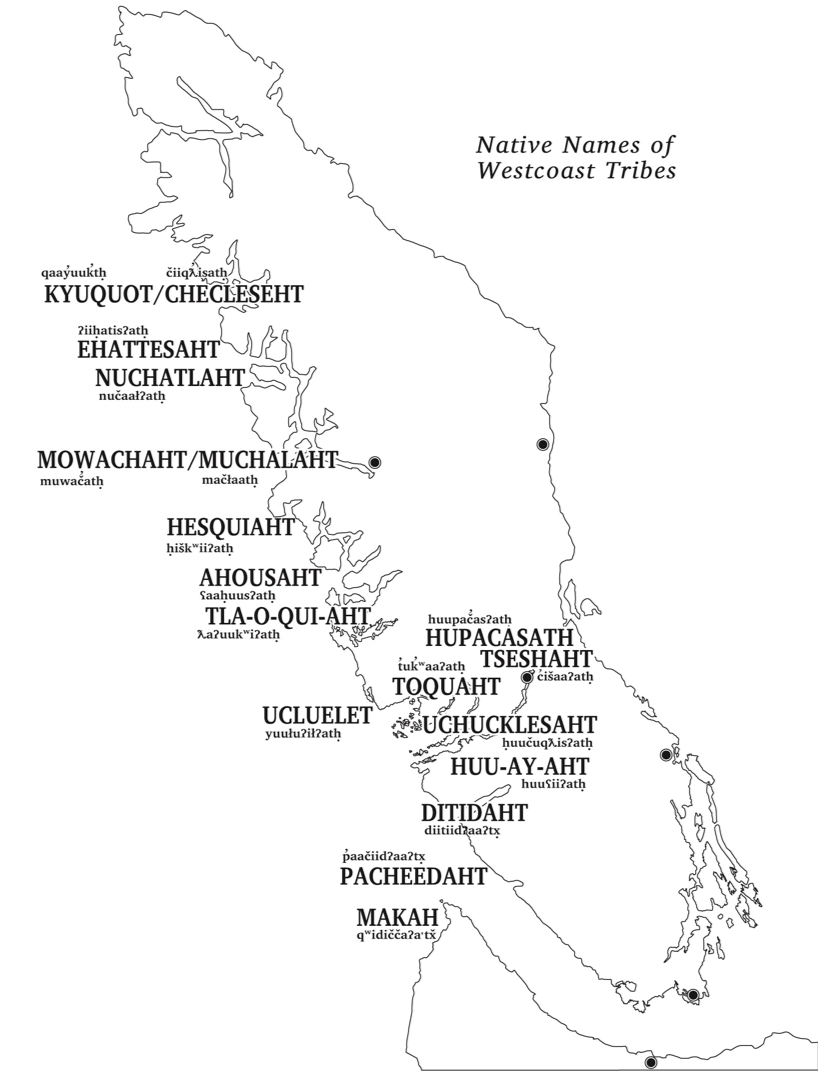
\includegraphics[height=\paperheight]{ncn-map.png}
%\end{figure}

\begin{tikzpicture}[remember picture, overlay]
  \node [anchor = north] at (current page.north)
     {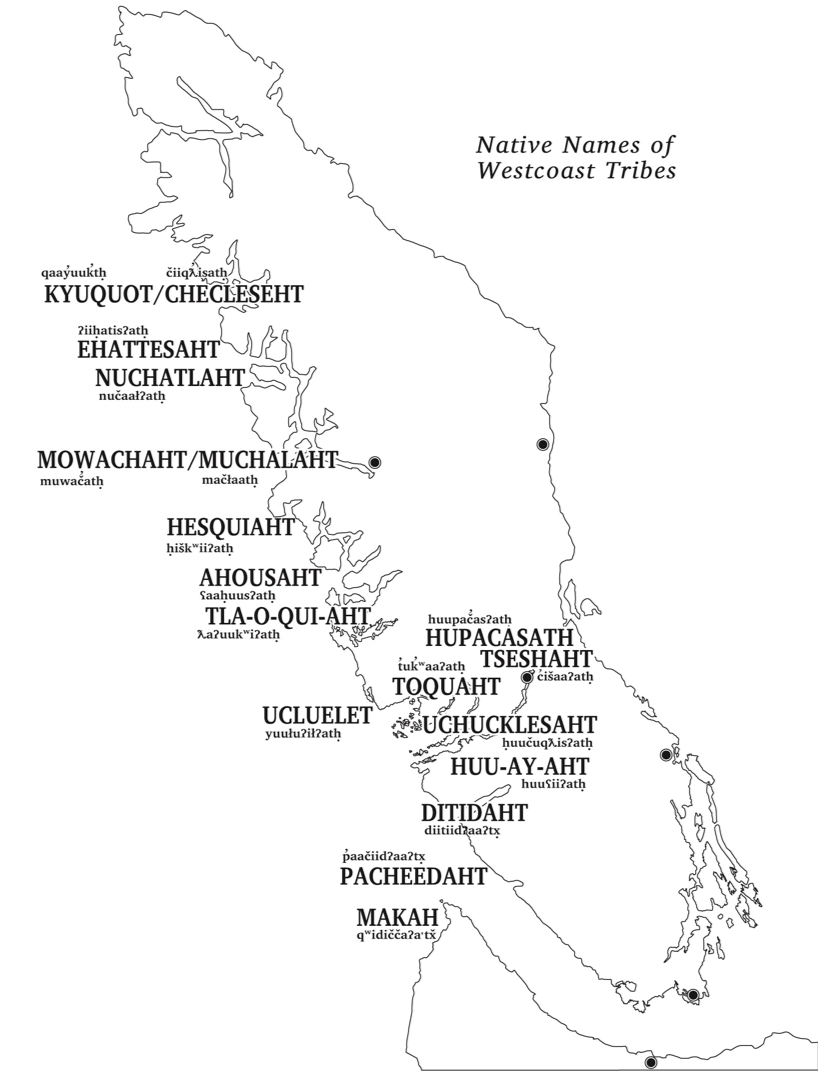
\includegraphics[height=\paperheight]{ncn-map.png}};
  \node [anchor=south west, inner sep=0pt]  at (current page.south west)
     {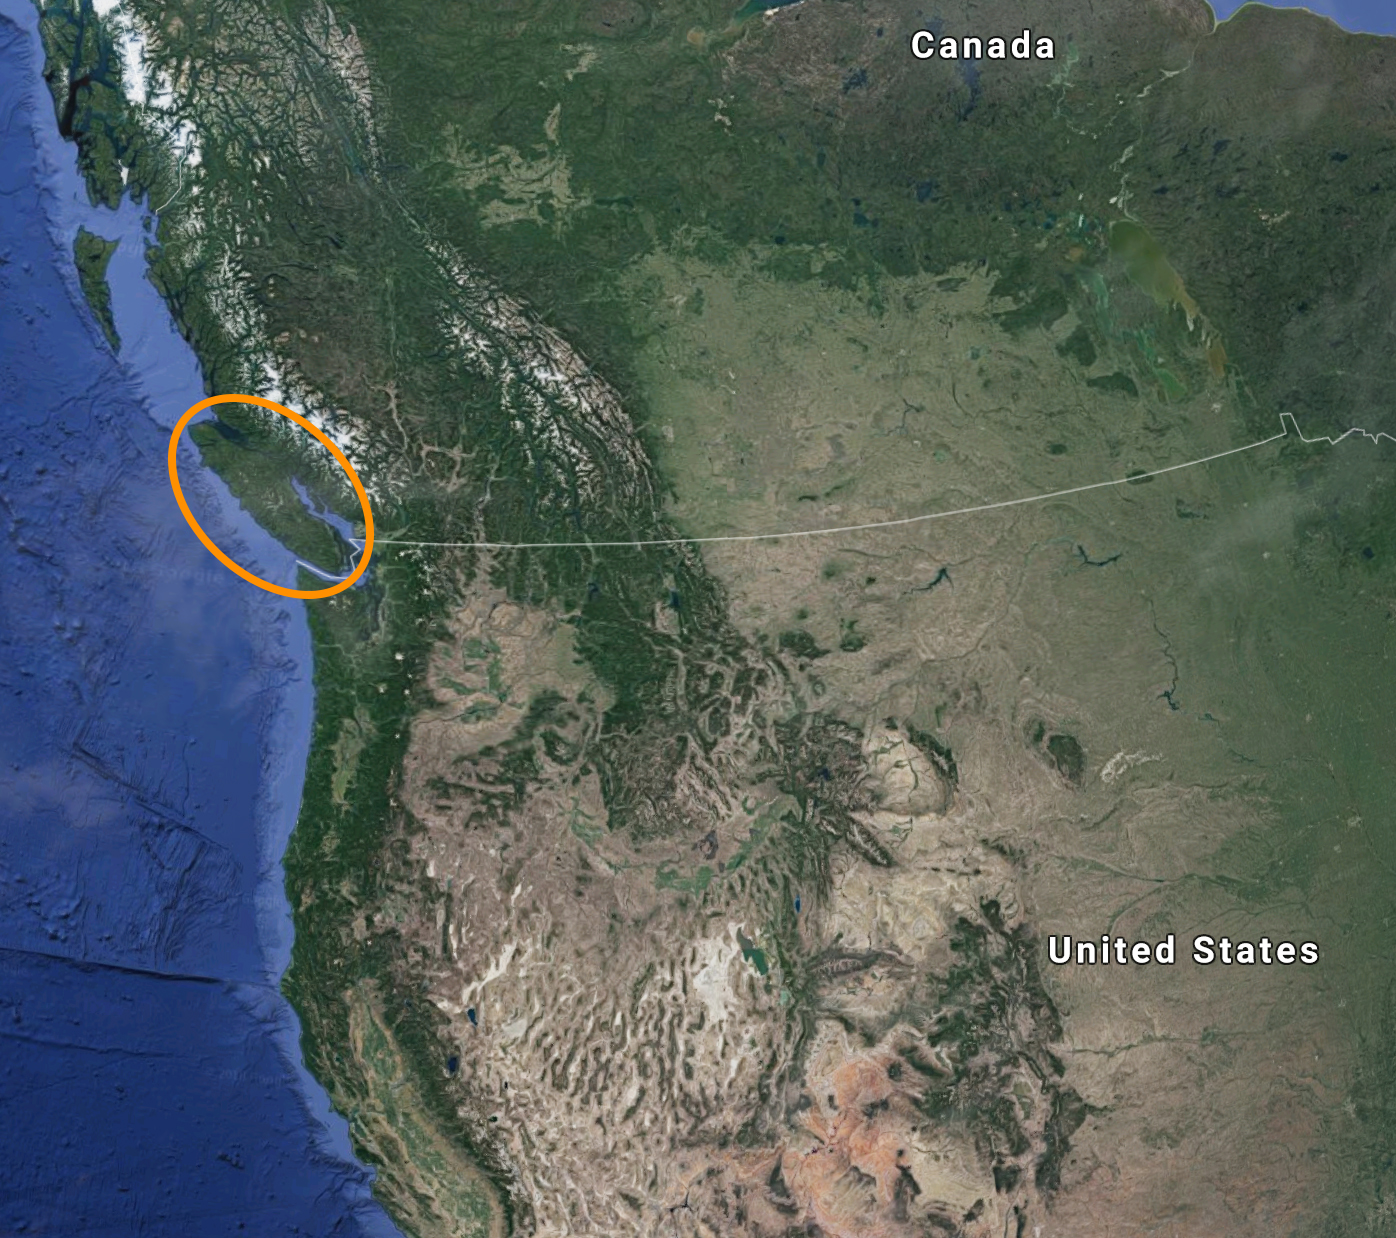
\includegraphics[height=3cm]{vanislandcircle.jpg}};
\end{tikzpicture}

\end{frame}

\begin{frame}

\begin{tikzpicture}[remember picture, overlay]
  \node [anchor = north] at (current page.north)
     {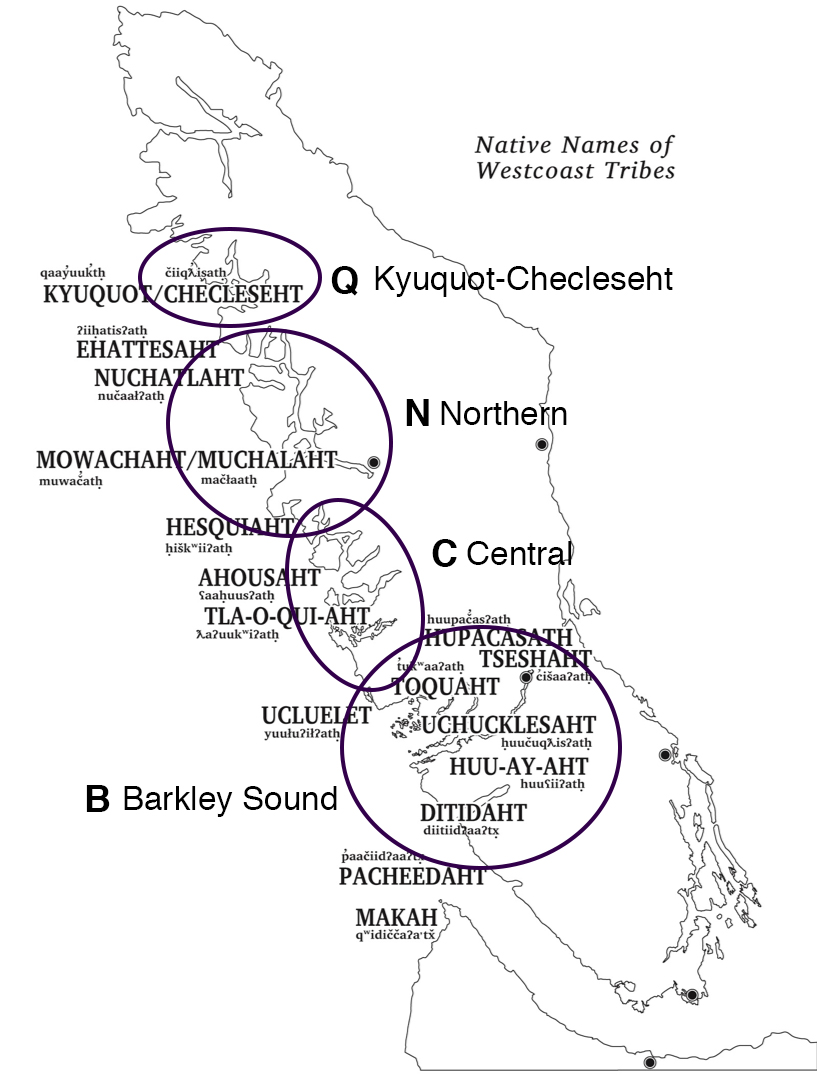
\includegraphics[height=\paperheight]{ncn-dialects.jpg}};
  \node [anchor=south west, inner sep=0pt]  at (current page.south west)
     {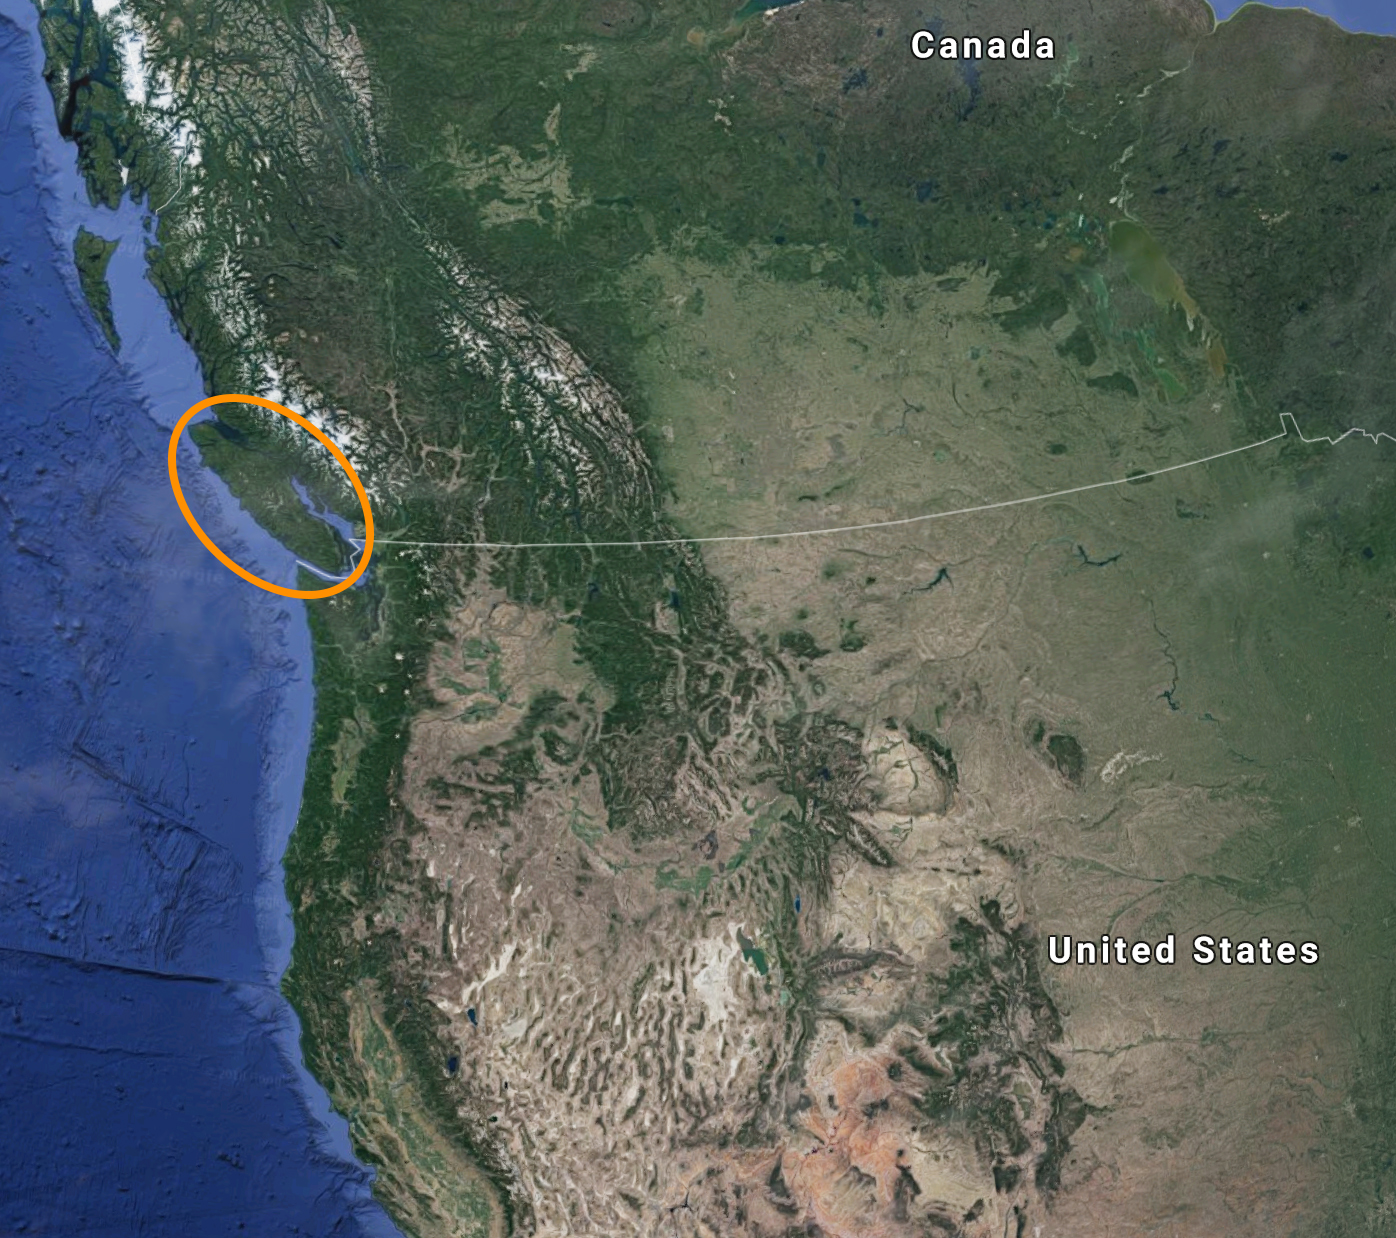
\includegraphics[height=3cm]{vanislandcircle.jpg}};
\end{tikzpicture}
\end{frame}

\begin{frame}{Introduction: Linguistic Background}
\begin{itemize}
\item Linguistic work dates to \cite{sapir1911}
\item Largest published texts in the Barkley Sound dialect \citep{sapir1939, sapir1955}
\item Recent syntactic work focused on the suffix ordering:
\begin{itemize}
\item \cite{waldie2004}: Suffix verbs (HPSG + linearization)
\item \cite{wojdak2005}: Suffix verbs (Minimalism)
\item \cite{woo2007b}: Adposition-like suffixes and argument-marking
\end{itemize}
\item Little analysis of the boundaries of clauses, clause/verb adjoining or coordination \citep{jacobsen1993}
\end{itemize}
\end{frame}

\begin{frame}{Methodology}
\begin{itemize}
\item Field work with speakers: describing images, question-answering, English translation, rephrasing, forced choice, linguist-constructed examples
\item Corpus study: Nootka Texts, community-produced texts, texts from other linguists, texts I collected from consultants
\item Analysis was done in an implemented DELPH-IN grammar, built using the HPSG formalism
\end{itemize}
\end{frame}

\chapter{The Basic Clause}
\label{ch:clause}

Before I turn to the meat of this dissertation, the multi-predicate constructions present in Nuuchahnulth, I will first give an overview of the language's basic clause structure and define some important terminology and lexical-syntactic distinctions present in the language. I will begin with the predicate/participant distinction (\S\ref{sec:clause:predp}, \S\ref{sec:clause:partp}), an important syntactic split which roughly maps to how verbs and nouns are used in English, but subsumes many lexical categories in Nuuchahnulth. I will then describe some special cases in which participant ordering is altered (\S\ref{sec:clause:partorder}). Finally I will look at second-position clausal clitics (\S\ref{sec:clause:cliticnormal}), and how the syntactic properties of Nuuchahnulth require special attention when modeling in HPSG (\S\ref{sec:clause:cliticmodifier}). I will interleave HPSG-style analyses with the data, but the descriptive facts should be available to linguists working in other formalisms.

\section{Syntactic Predicates} \label{sec:clause:predp}

Like many languages of the Pacific Northwest, Nuuchahnulth is predicate-initial and has a great deal of flexibility with respect to what parts of speech can be used predicatively \citep{jacobsen1979}. Because the term ``predicate" and its associated derivations (``predicative" and so on) are often ambiguous between syntactic and semantic concepts, I have found that linguists often talk past each other when trying to describe the syntax of the languages of South Wakashan. Throughout this work I will use special vocabulary to try to reduce this confusion.

I will reserve the word \textit{predicate} to refer to the syntactic component that heads a clause and connects components like subject and object to one another. In English, a syntactic predicate must be verbal, as in (\ref{ex:dogbarks},\ref{ex:grassgreen}). The verb `barks' serves as the predicate of (\ref{ex:dogbarks}), connecting it to the subject `the dog.' In (\ref{ex:grassgreen}), `is' serves as the sentential predicate, connecting its subject `the grass' to the complement `green.' I will refer to the units that predicates connect as \textit{participants}---this term encompasses both subject and complements. The sole participant of (\ref{ex:dogbarks}) is `the dog', and the participants of (\ref{ex:grassgreen}) are `the grass' and `green'.

\ex \label{ex:dogbarks}
[The dog]\textsubscript{participant} [barks]\textsubscript{predicate}.
\xe

\ex~ \label{ex:grassgreen}
[The grass]\textsubscript{participant} [is]\textsubscript{predicate} [green]\textsubscript{participant}.
\xe

In contrast to \textit{predicate} and \textit{participant}, which are syntactic concepts, I will use \textit{relation} and \textit{argument} to refer to their correlates in compositional semantics. The \textit{relation} is the atomic semantic unit that relates arguments to each other, typically represented with capital letters. For example, in (\ref{ex:dogbarks}), the English word \textit{barks} has the relation \textsc{bark}. Every semantically contentful morpheme has a relation, including syntactic participants (\textsc{dog}, \textsc{grass}, \textsc{green}).

Relations have some number of semantic \textit{arguments}. For example, \textsc{bark} can be modeled with two arguments: the event of barking, and the barker. This could be represented in a Neodavidsonian manner as \textsc{bark}(\textit{e}, \textit{x}). Note that the relation itself \textsc{bark} is at least conceptually separate from the number and type of its arguments. When I find it important to highlight the separation between the semantic relation and the number of its arguments, I may also refer to the relation as a \textit{predicate symbol}.\footnote{From terminology used by the DELPH-IN consortium. \url{http://moin.delph-in.net/ErgSemantics/Basics}} This semantic scheme is a simplification of the fuller semantic model that I will use later, Minimal Recursion Semantics \citep{copestake2005}.

It is important to keep in mind that the number of arguments that a semantic relation has is separate from its syntactic properties. The English predicate \textit{barks} may be represented as a semantic relation with two arguments \textsc{bark}(\textit{e}, \textit{x}). However, the syntactic non-predicate \textit{green} can be modeled in the same way: \textsc{green}(\textit{e}, \textit{x}). The syntactic properties of \textit{barks} and \textit{green}---predicate vs participant, which in English is straightforwardly subsumed into the verb vs adjective distinction---is separable from their semantic properties.

Though Nuuchahnulth has syntactic categories like verb, noun, and adjective, any of these may function as syntactic predicate or participant depending on where they fall in the sentence. The terms ``verb phrase," ``noun phrase," and ``adjective phrase" are valid insofar as they refer to a phrase headed by a verb, noun, or adjective, but they are not illuminating for determining syntactic roles, as any of these categories may be predicates.

In (\ref{ex:verbpred}), the verb \textit{n̓aacsiičiƛ} `see' is serving as the clausal predicate, while the clause \textit{hałmiiḥa quuʔas} `drowning person' is serving as the participant. In (\ref{ex:adjpred}), the adjective \textit{qʷac̓ał} `beautiful' is the predicate of the sentence, while the noun \textit{ḥaakʷaaƛ} `young girl' is the participant. In (\ref{ex:nounpred}) the noun \textit{pisatuwił} `gym' is the predicate and there are no participants. In this case, postposed \textit{ʔaanaḥi} `only' is a predicate-modifying adverb and not fulfilling any argument role of the relation \textsc{gym}.

\begin{comment}
While all three words have semantic relations (\textsc{see}, \textsc{drown}, \textsc{person}), only one is the syntactic predicate of the sentence.	
\end{comment}

\ex \label{ex:verbpred}
\begingl
\glpreamble n̓aacsiičiƛʔiš hałmiiḥa quuʔas. //
\gla n̓aacs-iˑčiƛ=ʔiˑš hałmiiḥa quuʔas //
\glb see-\textsc{in}=\textsc{strg.3sg} drowning person //
\glft `He sees a drowning person.' (\textbf{N}, Fidelia Haiyupis) //
\endgl
\xe

\ex~ \label{ex:adjpred}
\begingl
\glpreamble qʷac̓ałʔiš ḥaakʷaaƛʔi. //
\gla qʷac̓ał=ʔiˑš ḥaakʷaaƛ=ʔiˑ //
\glb beautiful=\textsc{strg.3} young.girl=\textsc{art} //
\glft `The young girl is beautiful.' (\textbf{C}, \textit{tupaat} Julia Lucas) //
\endgl
\xe

\ex~ \label{ex:nounpred}
\begingl
\glpreamble pisatuwiłma ʔaanaḥi. //
\gla pisatuwił=maˑ ʔaanaḥi //
\glb gym=\textsc{real.3} only //
\glft `It's only a gym.' (\textbf{B}, Marjorie Touchie) //
\endgl
\xe

Descriptively, it is sufficient to say that nouns, verbs, and adjectives may all be clausal predicates in Nuuchahnulth, in the same way that English requires clausal predicates to be verbs. Importantly, this data (including the modifying adverb in (\ref{ex:nounpred})), along with evidence from participant clauses (\S\ref{sec:clause:partp}), is sufficient to claim that nouns are events in Nuuchahnulth \citep{inman2018}. I will give my method for modeling this in (\S\ref{sec:clause:analysis}).

\section{Syntactic Participants} \label{sec:clause:partp}

Just as verbs, nouns, and adjectives may all be predicates, they may also all be participants. Example (\ref{ex:adjpred}) showed a straightforwardly nominal participant, the noun and article \textit{ḥaakʷaaƛʔi} `the young girl.' However, verbs (\ref{ex:verbpart}) and adjectives (\ref{ex:adjpart}) may also serve as participants.

\ex \label{ex:verbpart}
\begingl
\glpreamble ʔuḥʔiiš ʕiḥak kamatqukʔi. //
\gla ʔuḥ=ʔiˑš ʕiḥak kamatq-uk=ʔiˑ //
\glb be=\textsc{strg.3} cry.\textsc{dr} run-\textsc{dr}=\textsc{art} //
\glft `The running one is crying.' (\textbf{C}, \textit{tupaat} Julia Lucas) //
\endgl
\xe

\ex~ \label{ex:adjpart}
\begingl
\glpreamble wik̓iičʔaał ƛ̓iixc̓us ƛaƛuuʔi. //
\gla wik=!iˑč=ʔaał ƛ̓iixc̓us ƛaƛuu=ʔiˑ //
\glb \textsc{neg}=\textsc{cmmd.2pl}=\textsc{habit} laugh.at.\textsc{dr} other.\textsc{pl}=\textsc{art} //
\glft `Don't laugh at others.' (\textbf{C}, \textit{tupaat} Julia Lucas) //
\endgl
\xe

%\noindent TODO: confirm that (\ref{ex:adjpart}) is okay for sharing permissions, from a version of the Only Teachings.

As detailed in \cite{jacobsen1979} and \cite{wojdak2001}, when an adjective or verb is used as a participant, as in (\ref{ex:verbpart}, \ref{ex:adjpart}), the article \textit{=ʔiˑ} is required to make the sentence grammatical. When the participant is headed by a common noun, as in (\ref{ex:verbpred}), the article is optional. Proper nouns differentiate themselves from common nouns in that they may never take the article \citep{inman2018}. They are also never in predicate position.

My analysis of these facts is that the article \textit{=ʔiˑ} is in fact a relativizer that creates a participant from a notional predicate \cite{inman2018}.\footnote{This ultimately is original to Werle, \textit{p.c.}, who has also documented that \textit{=ʔiˑ} is morphologically in the same position as mood portmanteaus, and has supplanted the third person definite mood in some dialects.} Noun phrases may be relativized without the article, but other predicate phrases must be headed by the relativizing second position article \textit{=ʔiˑ}. That is, the semantics of the verb \textit{kamatquk} `run' and the noun \textit{pisatuwił} `gym' look like:

\ex~
\textsc{run}(\textit{e}, \textit{x})

\textsc{gym}(\textit{e}, \textit{x})
\xe

The event variable \textit{e} allows for tense, aspect, mood, and evidentiality values (TAME). This \textit{e} is also necessary for adverbial modification, which both verbs and nouns can undergo. However, when either type of word is used as a participant in the syntax, it is the variable (\textit{x}) that is needed by the semantics. \textit{=ʔiˑ} provides the relativizing function to accomplish this for all predicate types, and common nouns may undergo this process without an overt \textit{=ʔiˑ} attached. The analytical mechanisms for this will be addressed more fully in \S\ref{sec:clause:analysis}.

%\section{Participant Ordering} \label{sec:clause:partorder}

There is a strong tendency in Nuuchahnulth for each clause to have one overtly-expressed participant \citep[38]{rose1981} but if there are two participants expressed, they can come in any order. There is a preference in the southernmost dialects (Barkley sound and Central) for VSO ordering \citep[267]{jacobsen1993}, and a preference in the northern dialects (Northern and Kyuquot) for VOS ordering (Werle, \textit{p.c.}). This preference is not absolute, and to make the sentence unambiguous, speakers can use \textit{ʔuukʷił} to mark any non-highest argument \citep{woo2007b}.

\subsection{Participant Fronting}

It is possible for speakers to move a participant in front of the predicate for focus, as in (\ref{ex:focus}). This left-dislocated participant is notably outside the calculation for second position inflection (\S\ref{sec:clause:cliticnormal}).

\ex \label{ex:focus}
\begingl
\glpreamble ƛ̓aaq ʔuʔaatamin, waaʔaƛweʔin quʔušin. //
\gla ƛ̓aaq ʔu-ʔaˑta=(m)in waa=!aƛ=weˑʔin quʔušin //
\glb oil \textsc{x}-lack=\textsc{real.1pl} say=\textsc{now}=\textsc{hrsy.3} raven //
\glft ` ``We need oil," said Raven.' (\textbf{B}, Marjorie Touchie) //
\endgl
\xe

Wh-words and phrases also front, obligatorily, as in (\ref{ex:howmanydays}). In this case, the second position enclitics attach to the wh-word, so this fronting is ``inside" the second position calculation.

\ex \label{ex:howmanydays}
\begingl
\glpreamble qum̓aačłnik hił c̓uumaʕaas. //
\gla qum̓aa-čiˑł=nik hił c̓uumaʕaas //
\glb how.many-day=\textsc{pst.ques.2sg} be.at Port.Alberni //
\glft `How many days were you in Port Alberni?' (\textbf{Q}, Sophie Billy) //
\endgl
\xe

In addition to wh-words and focused participants, quantifiers tend to front as well (\ref{ex:uushilnofront}, \ref{ex:uushilfront}). It is possible in this case for the fronted quantifier to be either outside the syntactic scope of the second position enclitics (\ref{ex:uushilfront}) or inside it (\ref{ex:hishukfront}).

\ex \label{ex:uushilnofront}
\begingl
\glpreamble haʔukquuʔaała ʔuušił haʔum. //
\gla haʔuk=quu=ʔaała ʔuuš-L.(č)ił haʔum //
\glb eat.\textsc{dr}=\textsc{pssb.3}=\textsc{habit} some-\textsc{do.to} food //
\glft `He would only eat some things.' (\textbf{B}, Bob Mundy) //
\endgl
\xe

TODO:
\ex~ \label{ex:uushilfront}
\begingl
\glpreamble ʔuušił haʔukquuʔaała. //
\gla ʔuuš-L.(č)ił haʔuk=quu=ʔaała  //
\glb some-\textsc{do.to} eat.\textsc{dr}=\textsc{pssb.3}=\textsc{habit} //
\glft `He would only eat some things.' (\textbf{B}, Bob Mundy) //
\endgl
\xe

\ex~ \label{ex:hishukfront}
\begingl
\glpreamble hišuk̓ʷaƛʔišʔał kamitquk. //
\gla hišuk=!aƛ=ʔiˑš=ʔał kamitq-uk  //
\glb all-\textsc{now}=\textsc{strg.3}=\textsc{pl} run-\textsc{dr} //
\glft `Everyone is running.' (\textbf{N}, Fidelia Haiyupis) //
\endgl
\xe

I have not done a deep investigation into the conditions that determine whether the second position complex falls on the fronted quantifier or on the following predicate. In fact, this may vary by quantifier type. I have examples in my data of the fronted quantifier \textit{ʔuuš} taking the clitics (\ref{ex:uushfrontclitic}) or not (\ref{ex:uushfrontnoclitic}).

\ex \label{ex:uushfrontclitic}
\begingl
\glpreamble k̓umaaw̓it̓asʔaƛquu, n̓aačukitʔišʔaałʔał ʔin hiłʔapitʔaałʔał suč̓as, \textbf{ʔuušʔaƛquu wiikapuƛ}. //
\gla k̓um-aˑ-w̓it̓as=!aƛ=quu, n̓aačuk=(m)it=ʔiˑš=ʔaał=ʔał ʔin hił=!ap=(m)it=ʔaał=ʔał suč̓as, \textbf{ʔuuš=ʔaƛ=quu wiikapuƛ}  //
\glb point-\textsc{ct}-going.to=\textsc{now}=\textsc{pssb.3} look.\textsc{dr}=\textsc{pst}=\textsc{strg.3}=\textsc{habit}=\textsc{pl} \textsc{comp} be.at=\textsc{caus}=\textsc{pst}=\textsc{habit}=\textsc{pl} tree, \textbf{some=\textsc{now}=\textsc{pssb.3} pass.away.\textsc{mo}} //
\glft `If he is going to be pointer, they look to see if they put (someone) in a tree, if someone has passed away.' (\textbf{C}, \textit{tupaat} Julia Lucas) //
\endgl
\xe

\ex~ \label{ex:uushfrontnoclitic}
\begingl
\glpreamble ʔuuš n̓aacsamitsƛa hiłqḥ n̓ačiqs. //
\gla ʔuuš n̓aacsa=(m)it=s=ƛaˑ hił-(q)ḥ n̓ačiqs  //
\glb some see.\textsc{ct}=\textsc{pst}=\textsc{strg.1sg}=also be.at-\textsc{link} Tofino //
\glft `I also saw some at Tofino.' (\textbf{C}, \textit{tupaat} Julia Lucas) //
\endgl
\xe

This same pattern with respect to \textit{ʔuuš} is present in Sapir's original data.\footnotemark{} \textit{ʔuušił}, which is \textit{ʔuuš} `some' with the object marking \textit{-L.(č)ił} attached, behaves the same way in my data. \textit{ʔuušił} may be fronted without the second position enclitics, as already seen in (\ref{ex:uushilfront}), or it may then take the enclitics, as in (\ref{ex:uushilfrontclitic}) below. I could not find any \textit{ʔuušił} fronting in the Nootka Texts, so \textit{ʔuušił} fronting may represent a change in the language in the intervening generations.

\footnotetext{\noindent With the clitic complex:

\ex~ \label{ex:uushfrontcliticNT}
\begingl
\glpreamble ʔuušʔaƛ maqw̓in. //
\gla ʔuuš=!aƛ maq-w̓in  //
\glb some=\textsc{now} tie-middle //
\glft `Some are tied about the middle.' \citep[70]{sapir1955} //
\endgl
\xe

\noindent Without the clitic complex:

\ex~ \label{ex:uushfrontnocliticNT}
\begingl
\glpreamble ʔuuš saac̓inłšiʔaƛƛaa ʔaḥʔaa ƛ̓acʔii ƛ̓isitʔi sac̓up. //
\gla ʔuuš saac̓inł-šiƛ=!aƛ=ƛaa ʔaḥʔaa ƛ̓ac=ʔiˑ ƛ̓isit=ʔiˑ sac̓up  //
\glb some seafood.feast(?)-\textsc{mo}=\textsc{now}=also \textsc{dtop} fat=\textsc{art} white=\textsc{art} spring.salmon //
\glft `Some would start feasting with the fat, white-bodied tyee salmon.' \citep[22]{sapir1955} //
\endgl
\xe
}

\ex \label{ex:uushilfrontclitic}
\begingl
\glpreamble ʔuušiłqač̓a n̓aacsa. //
\gla ʔuuš-L.(č)ił=qač̓a n̓aacsa  //
\glb some-\textsc{do.to}=\textsc{infr.3} see.\textsc{ct} //
\glft `He must've seen something.' (\textbf{C}, \textit{tupaat} Julia Lucas) //
\endgl
\xe

I have no examples of the strong quantifier \textit{hišuk} `all' fronting without the second position complex, and it is possibly ungrammatical. The version of the strong quantifier in the Nootka texts, \textit{č̓uučk}, does not occur in a fronting environment where the enclitics unambiguously fall on the following predicate. (That is, in a case where the enclitic could not be a singly null-marked third person morpheme.)

My provisional analysis of these facts is to describe two types of fronting: (i) focus-fronting, which falls outside the calculation for second position enclitics and adds focus information to a word; and (ii) non-focus fronting, which falls inside the second position calculation and does not add focus. Non-focus fronting does not mean that the word is necessarily not focused, only that its left-extracted position is not giving it focus. This is significant as, according to many analyses, wh-words must be focused \citep[Chapter 5]{lambrecht1996}. Table \ref{table:fronting} gives the parts of speech that are compatible with each type of fronting.

\begin{table}[h]
\caption{Fronting properties of different words}
\begin{tabular}{l|l|l|l|l|} 
\cline{2-5}
                                         & nouns                & weak quantifiers      & strong quantifiers    & wh-words              \\ \hline
\multicolumn{1}{|l|}{Focus fronting}     & \cmark & \cmark & \xmark & \xmark \\ \hline
\multicolumn{1}{|l|}{Non-focus fronting} & \xmark & \cmark & \cmark & \cmark \\ \hline
\end{tabular} \label{table:fronting}
\end{table}

This discussion should not be considered definitive with respect to fronting and quantifier fronting in particular. Notably absent is \textit{ʔaya} `many', which I predict would pattern with \textit{hišuk}, but have not investigated. The claims with respect to the difference between \textit{hišuk} and \textit{ʔuuš} need checking, as well as claims about the status of these elements as having focus or not. For the purpose of this dissertation, I am only attempting to list the exceptions to the general rule that syntactic participants follow their predicate. Each of these cases is a special deviation from that general rule, and only happens under particular circumstances. I will ultimately model these as different types of extraction (\S\ref{sec:clause:analysis}).

%In addition to the special focus construction above, dependent clauses may realize their participants to the left without any special focus.

%TODO: Adam believes that participant-predicate ordering is possible in dependent clauses, citing ʔuyi. I believe that ʔuyi is an incipient adposition, and this is a postposition structure in these cases. It is extremely hard (impossible?) to find clear dependent clause participant-predicate ordering outside of ʔuyi. Ask Adam if he knows of non-ʔuyi examples.

\section{Second-position clitics} \label{sec:clause:cliticnormal}

The majority of clausal inflection in Nuuchahnulth is in a complex of second position enclitics which attach to the first word of the clause, modulo the left extraction seen in \S\ref{sec:clause:partp}. Table \ref{table:2pclitics} shows the ordering of the clitic complex, and is adapted from Adam Werle's grammar reference. A fuller list of these enclitics is given in Appendix \ref{appendix:grams}.

\begin{table}[h]
\centering
\caption{Order of second position clitics}
\label{table:2pclitics}
\begin{tabular}{c|c|c|c|c|c|c|c|c|c|c|}
\cline{2-11}
morph & =ʔaaqƛ & =!ap      & =!aƛ & =!at    & \begin{tabular}[c]{@{}c@{}}=uk\\ =ʔak\end{tabular} & =(m)it & \begin{tabular}[c]{@{}c@{}}=ʔiˑš\\ =maˑ\\ =ḥaˑ\\=$\emptyset$\\ ...\end{tabular} & =ʔaała   & =ʔał   & =ƛaˑ \\ \cline{2-11}
meaning  & \textsc{fut} & \textsc{caus} & \textsc{now}  & \textsc{pass} & \textsc{poss}  & \textsc{pst} & \begin{tabular}[c]{@{}c@{}}subject-mood\\ portmanteaus\end{tabular} & \textsc{habit} & \textsc{pl} & also \\ \cline{2-11}
\end{tabular}
\end{table}

The \textit{=$\emptyset$} morpheme, which indicates the third-person neutral mood, merits some special attention. While there is no phonological element associated with this inflection, all of the other enclitics appear in their typical order around where it would be. A predicate with no enclitic, or with one or more of the non-subject-mood enclitics (such as past, or habitual and plural) is always interpreted as being in the neutral mood with a third person subject. I do not put a \textit{=$\emptyset$} in my gloss lines, except below in (\ref{ex:2padjpart}) to show that it is notionally present. The syntactic information about neutral mood and 3rd person subject has to come from somewhere and this can be modeled as a phonologically empty morpheme providing it. I address this more in the implementation section (\S\ref{sec:clause:analysis}).

The examples I have given so far have all shown this clitic complex attaching directly to the clausal predicate. However, it may also attach to preceding adverbial modifiers (\ref{ex:2padvpred}), conjunctions (\ref{ex:2pconjpred}), and adpositions (\ref{ex:2padppred}).\footnote{The claim that (\ref{ex:2padppred}) is an adposition is somewhat controversial. \cite{woo2007b} analyzes these as little-\textit{v}, a category which does not exist in HPSG analyses. What this unit does is mark participants that fulfill a certain role with respect to the verb, similar to case-marking. An analysis that treats this particle as an adposition can generate the same set of sentences as a little-\textit{v} analysis, and is necessary within the HPSG framework. In this model, non-agentive arguments may be realized by a Participant Phrase or an Adposition Phrase headed by \textit{-L.(č)ił}. This means that in (\ref{ex:2padppred}), the word \textit{hiišił} is an adposition phrase modifying the following verb \textit{ʔiiqḥuk}.} Likewise, the relativizing enclitic article (\S\ref{sec:clause:partp}) may also attach to a preceding modifying adjective (\ref{ex:2padjpart}) and not directly to the head noun, as seen in (\ref{ex:adjpred}).

\ex \label{ex:2padvpred}
\begingl
\glpreamble y̓uuqʷaaʔaqƛs n̓aačuk. //
\gla y̓uuqʷaa=ʔaqƛ=s n̓aačuk  //
\glb also=\textsc{fut}=\textsc{1sg} look.for.\textsc{dr} //
\glft `I will also look for it.' (\textbf{C}, \textit{tupaat} Julia Lucas) //
\endgl
\xe

\ex~ \label{ex:2pconjpred}
\begingl
\glpreamble ʔaḥʔaaʔaƛna huʔacačiƛ ʔaḥkuu. //
\gla ʔaḥʔaaʔaƛ=naˑ huʔa-ca-čiƛ ʔaḥkuu  //
\glb and.then=\textsc{strg.1pl} back-go-\textsc{mo} \textsc{d1} //
\glft `And then we came back here.' (\textbf{C}, \textit{tupaat} Julia Lucas) //
\endgl
\xe

%\ex~ \label{ex:2padppred}
%\begingl
%\glpreamble hiišiłʔaƛ ʔiiqḥuk, ʔumaḥsiičiƛs ḥaakʷaaƛ. //
%\gla hiš-L.(č)ił=ʔaƛ ʔiiqḥ-uk ʔumaḥsiičiƛ=s ḥaakʷaaƛ  //
%\glb all-\textsc{do.to}=\textsc{now} tell-\textsc{dr} want.to.marry.\textsc{mo}=\textsc{strg.1sg} young.woman //
%\glft `He told everyone, ``I want to marry that young woman." ' (\textbf{C}, \textit{tupaat} Julia Lucas) //
%\endgl
%\xe

\ex~ \label{ex:2padppred}
\begingl
\glpreamble ʔuukʷiłw̓it̓asaḥ haaʕin čims. //
\gla ʔu-L.(č)ił-w̓it̓as=(m)aˑḥ haaʕin čims  //
\glb \textsc{x}-\textsc{do.to}-going.to=\textsc{real.1sg} invite.\textsc{dr} bear //
\glft `I'm going to invite bear' (\textbf{B}, Marjorie Touchie) //
\endgl
\xe

\ex~ \label{ex:2padjpart}
\begingl
\glpreamble m̓uyaa ḥaa ƛaʔuuʔi maḥt̓ii. //
\gla m̓u-(y)aˑ(=$\emptyset$) ḥaa ƛaʔuu=ʔiˑ maḥt̓iˑ  //
\glb burn-\textsc{cv}(=\textsc{neut.3}) \textsc{d3} other=\textsc{art} house //
\glft `The other house was burning.' (\textbf{C}, \textit{tupaat} Julia Lucas) //
\endgl
\xe

%[[TODO: Find a two-word analytic \textit{ʔuukʷił} version of (\ref{ex:2padppred}), which only has the suffix version \textit{-L.čił}.]].

Every clause in Nuuchahnulth contains an enclitic, even if it is only the notional =$\emptyset$ third person neutral enclitic. With the exception fo extraction (\S\ref{sec:clause:partp}), the enclitic always appears on the first word of the clause, which is either the predicate or a preceding adverb. Together with the restrictions on syntactic predicates, I use this data to claim that the clitic complex is the syntactic head of the clause in Nuuchahnulth, and the clitic complex then selects for predicates. That is, the second position enclitic complex is the auxiliary head of a clause, and inherits its valence (number of complements) from the predicate, which also provides the main semantic relation of the clause. Because of its second position properties, this analysis of the Nuuchahnulth clitic requires some special attention in HPSG (\S\ref{sec:clause:analysis}), but descriptively I can stop at calling the enclitic complex the head of the Nuuchahnulth clause.

One final fact about the clause worth mentioning is clitic spreading. The presence of a clitic \textit{in situ} within the second position complex is required. If the clause is passive, the passive morpheme must appear within the complex, and so on. However, some of these clitics may appear multiply within a clause: first in the second position enclitic complex, and then later on the predicate or predicates of the sentence. This occurs in cases where there is a preposed adposition\footnote{For the argument that \textit{ʔuyi} is an adposition, see \S\ref{sec:link:uyi}.} (\ref{ex:doubleatluyi}), a preposed adverb (\ref{ex:doubleatlyuuqwaa}, \ref{ex:doubleap}), a preposed quantifier (\ref{ex:doubleatuush}),\footnote{Note that in this instance the quantifier has a linker attached. The semantics of the linker will be addressed in \S\ref{sec:link}.} or a clefting construction (\ref{ex:doubleatuh}). In all these cases, there is a syntactic reason for the second position clitic complex to fall on something other than the main predicate of the clause, and some of the clitics may appear multiply: within the second position complex (obligatorily) and on the main predicate (optionally). To my knowledge, the only clitics that ``spread" like this are \textit{=!aƛ} `now' (\ref{ex:doubleatluyi}, \ref{ex:doubleatlyuuqwaa}), \textit{=!at} \textsc{passive} (\ref{ex:doubleatuush}, \ref{ex:doubleatuh}), and \textit{=!ap} \textsc{causative} (\ref{ex:doubleap}). I will come back to how the multiple instances of the valence-altering clitics \textit{=!at} and \textit{=!ap} functions within serialization structures in \S\ref{sec:sv:valence}. %\footnote{There will be a significant discussion on multiple instances of the causative morpheme in \S\ref{sec:sv:valence}, which I treat differently. All instances of multiple causative morphemes appear to show the causative attaching to and modifying different predicates. This differs from \textit{=!aƛ} `now' and \textit{=!at} \textsc{passive}, where the morphemes are attaching to adpositions (\ref{ex:doubleatl}) or fronted quantifiers (\ref{ex:doubleatpass}).}

\ex \label{ex:doubleatluyi}
\begingl
\glpreamble ʔuyiʔeƛna hawiiʔeƛ kaaƛḥšiʔeƛquu. //
\gla ʔuyi=ʔaƛ=naˑ hawiiƛ=!aƛ kaƛḥ-šiƛ-LS=!aƛ=quu  //
\glb at.a.time=\textsc{now}=\textsc{neut.1pl} finish=\textsc{now} be.light-\textsc{mo}-\textsc{grad}=\textsc{now}=\textsc{pssb.3} //
\glft `We stop when it starts getting light.' (\textbf{C}, \textit{tupaat} Julia Lucas) //
\endgl
\xe

%huʔacačiʔeƛweʔin hiʔiisʔaƛ quʔušin.
%ʔa-ca-čiƛ=!aƛ=weˑʔin hiłʔiis=!aƛ quʔušin
%He came back to where Raven was. MT

\begin{comment}
\ex \label{ex:doubleatl2}
\begingl
\glpreamble ʔuḥʔaƛ tiic̓̌ap̓aƛ hałmiiḥa. //
\gla ʔuḥ=!aƛ tiic=!ap=!aƛ hałmiiḥa  //
\glb be=\textsc{now} alive.\textsc{dr}=\textsc{caus}=\textsc{now} drown.\textsc{ct} //
\glft `He made him alive from drowning.' (\textbf{C}, \textit{tupaat} Julia Lucas) //
\endgl
\xe
\end{comment}

\ex~ \label{ex:doubleatlyuuqwaa}
\begingl
\glpreamble y̓uuqʷaaʔaƛweʔin ƛ̓iḥmam̓it ʔunaak̓aƛ yaaqʷapakʔitq k̓ʷičiƛ. //
\gla y̓uuqʷaa=!aƛ=weˑʔin ƛ̓iḥmam̓it ʔu-naˑk=!aƛ yaqʷ-L.apak=ʔiˑtq k̓ʷi-čiƛ  //
\glb also=\textsc{now}=\textsc{hrsy.3} woodpecker \textsc{x}-have=\textsc{now} who-beyond=\textsc{defn.3} stick-\textsc{mo} //
\glft `And also Woodpecker had his man who was best of all in marksmanship.' (\textbf{B}, \citealt[50]{sapir1939}) //
\endgl
\xe

%. NT 1939 p50

\begin{comment}
\ex~ \label{ex:doubleap}
\begingl
\glpreamble hišuk̓ap̓aƛ witkʷaaʔap ʔin wikmaḥsap̓aƛ, ḥaakʷaaƛsma. //
\gla hišuk=!ap=!aƛ witkʷaa=!ap ʔin wik-maḥsa=!ap=!aƛ, ḥaakʷaaƛ-sma  //
\glb all=\textsc{caus}=\textsc{now} destroy=\textsc{caus} \textsc{comp} \textsc{neg}-want.to=\textsc{caus}=\textsc{caus} young.woman-protective.of //
\glft `Everyone destroyed the wharf because they wanted her to marry, they were stingy of the girl.' (\textbf{C}, \textit{tupaat} Julia Lucas) //
\endgl
\xe
\end{comment}

%saač̓iyapitapsi makułʔi ʔuuʔiʔiłʔap. NT 1939 p. 140

\ex~ \label{ex:doubleatuush}
\begingl
\glpreamble ʔuušḥʔatquus n̓aačuk̓ʷat, ʔiiqḥuk̓um ʔanis weʔič. //
\gla ʔuuš-(q)ḥ=!at=quus n̓aačuk=!at ʔiiqḥuk=!um ʔani=s weʔič  //
\glb some-\textsc{link}=\textsc{pass}=\textsc{pssb.1sg} look=\textsc{pass} tell.\textsc{dr}=\textsc{cmmd.go} \textsc{comp}=\textsc{1sg} sleep.\textsc{dr} //
\glft `If anyone is looking for me, tell them I'm sleeping.' (\textbf{B}, Marjorie Touchie) //
\endgl
\xe

\ex~ \label{ex:doubleatuh}
\begingl
\glpreamble ʔuḥʔatsʔał ʔumʔiiqsakqs m̓aw̓aaʔat ƛiisuwił. //
\gla ʔuḥ=!at=s=ʔaˑł ʔumʔiiqsu=ʔak=qs m̓aw̓aa=!at ƛiisuwił  //
\glb be=\textsc{pass}=\textsc{strg.1sg}=\textsc{habit} mother=\textsc{poss}=\textsc{defn.1sg} bring.\textsc{pf}=\textsc{pass} school //
\glft `It's my mother who brings me to school.' (\textbf{N}, Fidelia Haiyupis) //
\endgl
\xe

%ʔuḥʔats ʕiniiƛ ƛawiičiʔat kamitquk JL

\begin{comment}
\ex~ \label{ex:doubleatgeneric}
\begingl
\glpreamble ʔayaqḥʔatna huḥtak̓at. //
\gla ʔaya-(q)ḥ=!at=naˑ huḥtak=!at  //
\glb many-\textsc{link}=\textsc{pass}=\textsc{neut.1pl} learn=\textsc{pass} //
\glft `Many know.' (\textbf{B}, Sarah Webster) //
\endgl
\xe
\end{comment}


\ex~ \label{ex:doubleap}
\begingl
\glpreamble ʔiqsiłapƛaa hinʔatap ḥiin̓aakʔi.\footnotemark{} //
\gla ʔiqsiła=!ap=ƛaa hinʔatap ḥiin̓a=ʔak=ʔiˑ  //
\glb still=\textsc{caus}=also in.water.\textsc{caus} quartz=\textsc{poss}=\textsc{art} //
\glft `Again they put the quartzes under water.' (\textbf{B}, \citealt[60]{sapir1955}) //
\endgl
\xe
%wik̓aƛ̓apuƛ ʔaanaḥap t̓aat̓aapata.

\footnotetext{Corrected to ḥiin̓aakʔi from hiinaakʔi.}

It is significant that in all the above examples, this syntactic doubling does not indicate any semantic doubling. In all of the examples, the unit that the second position enclitic attaches to is not notionally compatible with the semantics of ``now," or the application of a causative or passive.\footnote{The possible exception to this is (\ref{ex:doubleatluyi}), if \textit{ʔuyi} is understood as a full verb. As mentioned above, I believe it is an adposition.} That is, the examples here all show a strictly syntactic, not semantic, phenomenon.\footnote{This is not the case under serialization, where causative and passive morphology may affect only one verb under serialization. This will be addressed in \S\ref{sec:sv:valence}.} This syntactic ``doubling" is restricted to the clause in which the semantics of the morpheme apply. This can be seen in (\ref{ex:decidetogo}, \ref{ex:*decidetogo}) below, where the \textit{=!aƛ} `now' morpheme cannot be introduced in the subordinate clause, where it would alter the semantics in a bizarre or unintelligible way.

\ex \label{ex:decidetogo}
\begingl
\glpreamble t̓apatšiʔaƛs ʔucačiƛ c̓aʔakʔi. //
\gla t̓apat-šiƛ=!aƛ=s ʔu-ca-čiƛ c̓aʔak=ʔiˑ //
\glb think-\textsc{mo}=\textsc{now}=\textsc{strg.1sg} \textsc{x}-go-\textsc{mo} river=\textsc{art} //
\glft `I decided to go to the river.' (\textbf{N}, Fidelia Haiyupis) //
\endgl
\xe

\ex~ \label{ex:*decidetogo}
\begingl
\glpreamble *t̓apatšiʔaƛs ʔucačiʔaƛ c̓aʔakʔi. //
\gla *t̓apat-šiƛ=!aƛ=s ʔu-ca-čiƛ=!aƛ c̓aʔak=ʔiˑ //
\glb think-\textsc{mo}=\textsc{now}=\textsc{strg.1sg} \textsc{x}-go-\textsc{mo}=\textsc{now} river=\textsc{art} //
\glft Intended: `I decided to go to the river.' (\textbf{N}, Fidelia Haiyupis) //
\endgl
\xe

\section{Second position verbal suffixes} \label{sec:clause:2pv}

Another set of second position elements are verbal suffixes. Nuuchahnulth has a series of suffixing elements that attach to the leftmost item in their object. Although it is outside the scope of this dissertation, there is good independent reason to believe that these elements are suffix-like in the traditional sense, rather than clitic-like. Briefly, they are more tightly phonologically integrated into their root than the clausal clitics (\S\ref{sec:clause:cliticnormal}), they can attach to bound roots (the clausal clitics may not), and they occasionally produce unpredictable semantics. I will here simply assume their status as lexical suffixes with second position properties, rather than phrasal clitics.

The second position suffixes have been the locus of a fair amount of recent linguistic research in Nuuchahnulth, notably \cite{waldie2004}, \cite{wojdak2005}, and \cite{woo2007b}. \cite{wojdak2005} gives a detailed account of these suffixes under the Minimalist program. \cite{wojdak2005} breaks these suffixes into two broad categories, affixal main predicates (in my terminology, verbs which take participant complements) and affixal auxiliary predicates (verbs which take a predicate complement). I think this split is partially correct (although I will add one more basic category), but disagree with her overall account in at least one important way that are not attributable to our difference in framework. \citeauthor{wojdak2005} claims that these suffixes are insensitive to the category they attach to (p.\ 52--54). I think this claim is too general. Her argument comes down to two main predicate suffixes, \textit{-ʕiƛ} `find' and \textit{-atuł} `dream of,' which can attach to verbs (p.\ 159). While this may be the case for these particular verbs, it is not the general case for suffix verbs, which for the most part either strictly take referential semantic arguments (the ``main predicates") or eventive semantic arguments (the ``auxiliary predicates"). For the small number of suffixes, like \textit{-ʕiƛ} `find' and \textit{-atuł} `dream of', that can take both eventive and referential arguments can either be analyzed as a supertype of the two more specific lexical categories, or as lexically ambiguous. In either case, these are the minority. I will address the attachment properties of both main predicate suffixes (\ref{sec:clause:2pv:mainpredicate}) and auxiliary predicate suffixes (\ref{sec:clause:2pv:auxiliary}) independently below.

%I believe the different classes of these suffixes each have different attachment properties. I will focus here on these distinctions, and not mention the scoping issues (especially with respect to the negator), which \citeauthor{wojdak2005} goes into in depth.

I break the second position suffixes broadly into three categories: (i) main predicate suffixes (\S\ref{sec:clause:2pv:mainpredicate}), which are transitive (and ditransitive) verbs that take referential complements; (ii) auxiliary predicate suffixes (\S\ref{sec:clause:2pv:auxiliary}), which modify predicates they subject control, and typically have modal or modal-like semantics, and (iii) location suffixes (\S\ref{sec:clause:2pv:loc}), which \cite{wojdak2005} treats as a subtype of the main predicate suffixes, but I believe have some special properties that differentiate them. Finally, I note some suffixes which do not appear to fall under any of the above categories (\S\ref{sec:clause:2pv:additional}). It is probable that this list is incomplete or in error in some parts, and there is further specialization within each of these categories. I am only intending here to give an overview of these categories, which will help illuminate later analyses.

\subsection{Main predicate suffixes} \label{sec:clause:2pv:mainpredicate}

The main predicate suffixes are semantic units that relate referents (not events) to one another. They can be either transitive or ditransitive. That is, their basic semantic type is:

\ex
\textsc{relation}(\textit{e}, \textit{x1}, \textit{x2}, (\textit{x3}))
\xe

This includes relations such as \textsc{have}, \textsc{take}, \textsc{find}, \textsc{gather/hunt}, \textsc{consume}, and so on (expressed with -\textit{naˑk}, \textit{-L.!iƛ}, \textit{-L.waƛ}, \textit{-R.!iiḥ}, and \textit{-iis} respectively). The only ditransitive in this group that I know of is the suffix \textit{-ayiˑ}, which expresses the relation \textsc{give}.

I will use the suffix verb \textit{-naˑk} `have' to illustrate the syntactic attachment properties of these suffixes. Each sentence in (\ref{ex:havesong}--\ref{ex:havetwolongsongs}) shows a longer direct object of `have': song, two songs, two long songs. The suffix verb always attaches to the first element in the object.

\ex \label{ex:havesong}
\begingl
\glpreamble nuuknaaks. //
\gla nuuk-naˑk=s //
\glb song-have=\textsc{strg.1sg} //
\glft `I have a song/songs.' (\textbf{N}, \textit{yuułnaak} Simon Lucas) //
\endgl
\xe

\ex~ \label{ex:havetwosongs}
\begingl
\glpreamble ʔaƛanaks nuuk. //
\gla ʔaƛa-naˑk=s nuuk //
\glb two-have=\textsc{strg.1sg} song //
\glft `I have two songs.' (\textbf{N}, \textit{yuułnaak} Simon Lucas) //
\endgl
\xe

\ex~ \label{ex:havetwolongsongs}
\begingl
\glpreamble ʔaƛanaks y̓aaq nuuk. //
\gla ʔaƛa-naˑk=s y̓aaq nuuk. //
\glb song-have=\textsc{strg.1sg} //
\glft `I have two long songs.' (\textbf{N}, \textit{yuułnaak} Simon Lucas) //
\endgl
\xe

Instead of attaching to a semantically contentful word, the suffix verb can attach to the empty root \textit{ʔu-}, which I gloss as \textsc{x}. In this construction, the object can either appear after (\ref{ex:havechant}) or be dropped (\ref{ex:haveit}). Syntactically, the second position effect persists, if the \textit{ʔu-} root is seen as syntactically part of the object, but carrying no semantic content.

\ex \label{ex:havechant}
\begingl
\glpreamble ʔunaaks c̓iiqy̓ak. //
\gla ʔu-naˑk=s c̓iiq-y̓ak //
\glb \textsc{x}-have=\textsc{strg.1sg} chant-for //
\glft `I have a chant.' (\textbf{N}, \textit{yuułnaak} Simon Lucas) //
\endgl
\xe

\ex~ \label{ex:haveit}
\begingl
\glpreamble ʔiiqḥiis ʔunaˑk. //
\gla ʔiiqḥii=s ʔu-naak //
\glb still=\textsc{strg.1sg} \textsc{x}-have //
\glft `I still have it.' (\textbf{N}, Fidelia Haiyupis) //
\endgl
\xe

It is also possible for these elements to attach to an adverb. In this case, the adverb is always modifying the verb's event, as in (\ref{ex:longtimedog}).

\ex \label{ex:longtimedog}
\begingl
\glpreamble qiinaakitaḥ ʕiniiƛ. //
\gla qii-naˑk=(m)it=(m)aˑḥ ʕiniiƛ //
\glb long.time-have=\textsc{pst}=\textsc{real.1sg} dog //
\glft `I have had a dog for a long time.' (\textbf{B}, Bob Mundy) //
\endgl
\xe

This second position only scopes over the VP, and is separate from the clausal second position (\S\ref{sec:clause:cliticnormal}). As seen already in (\ref{ex:haveit}) and (\ref{ex:badnews}), the clausal second position occurs separately from the second position of the suffix verb. I give two more examples of this clear separation in with a negator (\ref{ex:badnews}) and a conjunction (\ref{ex:mightnotgive}) below.

%ʔaḥʔaaʔaƛna huʔacačiƛ ʔaḥkuu.
%Then we came back here.

\ex \label{ex:badnews}
\begingl
\glpreamble wik̓ii ʔaanamac̓uk p̓išaq ʔuyaqḥmis. //
\gla wik=!iˑ ʔana-L.mac̓uk.\textsc{dr} p̓išaq ʔuyaqḥ-mis //
\glb \textsc{neg}=\textsc{cmmd.2sg} only-talk.about bad news-\textsc{nmlz} //
\glft `Don't only talk about bad news.' (\textbf{C}, \textit{tupaat} Julia Lucas) //
\endgl
\xe

\begin{comment}
\ex \label{ex:mightnotgive}
\begingl
\glpreamble wikcumʔick huʔayi siičił waaʔaƛ. //
\gla wik-cum=ʔick huʔa-ayiˑ si-L.(č)ił waa=!aƛ //
\glb \textsc{neg}-might=\textsc{real.2sg} back-give \textsc{1sg}-\textsc{do.to} say=\textsc{now} //
\glft ` ``You might not give it back," he said.' (\textbf{C}, \textit{tupaat} Julia Lucas) //
\endgl
\xe
\end{comment}

\ex~ \label{ex:mightnotgive}
\begingl
\glpreamble ʔaḥʔaaʔaƛs ʔuukʷiił yaqwiiʔakqs ƛiisyuu pikčas. //
\gla ʔaḥʔaaʔaƛ=s ʔu-L.(č)iił yaq-(t)wii=ʔak=qs ƛiis-yuu pikčas //
\glb and=\textsc{strg.1sg} \textsc{x}-make what-do.first=\textsc{poss}=\textsc{defn.1sg} mark-\textsc{rs} picture //
\glft `And then I made my first picture.' (\textbf{N}, Fidelia Haiyupis) //
\endgl
\xe

These suffixes typically cannot attach to verbs, as seen below. This makes sense if their semantics expect a referent and not event. With nouns and adjectives, syntactic incorporation incorporates a referent (either that of the noun or of the adjective's modifyee). With verbs, there is no clear referent to compose with.

[[TODO: Examples from Julia, MT]]

Despite this general rule, some suffixes in this class idiosyncratically attach to verbal roots with unpredictable semantics. For instance, the suffix \textit{-L.!iƛ} `take' can idiosyncratically attach to the verb root \textit{n̓ikʷ-} `claw' to yield \textit{n̓iik̓ʷiƛ} `take by clawing.' This does not describe two actions: a clawing event, and then taking the result of that event or a participant, but one event of seizing in talons or claws. This instrumentative reading is completely unpredictable. Another example is the suffix \textit{-uʔał} `see', which I have most commonly encountered attaching to the verb root \textit{n̓ač-} to form \textit{n̓ačuʔał} `see (esp.\ a person).'\footnote{Though less common, is possible for \textit{-uʔał} to attach in the ``normal" way of a suffix verb as well, as in (\ref{ex:sawabigman}).

\ex \label{ex:sawabigman}
\begingl
\glpreamble ʔiiḥuʔałitaḥ quuʔas ʔukłaa Adam. //
\gla ʔiiḥ-uʔał=(m)it=(m)aˑḥ quuʔas ʔu-(k)łaˑ Adam //
\glb big-see=\textsc{pst}=\textsc{real.1sg} person \textsc{x}-call Adam //
\glft `I saw a big person named Adam.' (\textbf{B}, Marjorie Touchie) //
\endgl
\xe
} This lexical doubling `see-see' is again unpredictable. I treat all these cases of verb attachment as unanalyzable, single lexical items.

It also seems to be the case that verbal attachment was either a more productive property or more widespread in the lexicon in the past, and I believe this is what \cite{wojdak2005} picks up on in her dissertation. Verbal attachment does happen, I am merely claiming that it has special properties. [[TODO: pick up here]]

NT:
ʔaḥʔaaʔaƛ ƛiḥnaak̓aƛ hinatimyisnak̓aƛ hitaqƛiłʔatḥʔi maatmaas.
ciqnaak
ciqnaak̓aƛ ʔaḥʔaa y̓uuqʷaa huuʕiiʔatḥ.

This class of suffixes also attaches to root forms, when available. This can be seen in words like \textit{quuʔac-iic} `belonging to a Native person,' where the bound root form \textit{quuʔac} `person' is used instead of the free form \textit{quuʔas}. This also occurs with \textit{łuč-naak} `have a wife,' where the bound root form \textit{łuč} `woman' is used instead of the free form \textit{łuucsma}. If a word does not have a special bound form, the free form is used.

The first class of second position suffixes, then, are transitive and ditransitive verbs that take referential arguments. They attach to the first element of their complement, either the noun itself or a modifying adjective, or they may attach to the semantically empty root \textit{ʔu-} and take complements in the normal manner. They may also attach to an adverb, in which case the adverb modifies the semantics of the suffix verb itself. They do not generally attach to verbs, and when they do it is both syntactically and semantically unpredictable.

\subsection{Auxiliary predicate suffixes} \label{sec:clause:2pv:auxiliary}

The second class is auxiliary predicate suffixes. These tend to have modal or modal-like semantics, and relate a referent to an even. That is, the basic semantics are as below.

\ex
\textsc{relation}(\textit{e}, \textit{x1}, \textit{e2})
\xe

They are also all subject control verbs \citep[p.\ 160]{wojdak2005}: Their subject must match the subject of their complement predicate. Syntactically, this means that the \textit{x1} of the relation above is always identified with the subject of whatever the \textit{e2} is.

Syntactically, these suffixes behave in some similar ways to the transitive verb suffixes. As I used \textit{-naˑk} to exemplify the transitive verb suffixes, I will use \textit{-maḥsa} `want to do' to exemplify this category of suffix. The most straightforward use of this suffix is to attach to a verbal predicate, as in (\ref{ex:wanttograb}). As a suffix subject control verb, the subject of the wanting event in (\ref{ex:wanttograb}) is the same as the subject of the grabbing event.

\ex \label{ex:wanttograb}
\begingl
\glpreamble hišuk̓aƛ čaakupiiḥ sukʷiƛmaḥsa ḥaa p̓aacac̓umʔi //
\gla hišuk=!aƛ čaakupiiḥ su-kʷiƛ-maḥsa ḥaa p̓aacac̓um=ʔiˑ //
\glb all=\textsc{now} man.\textsc{pl} hold-\textsc{mo}-want.to.do \textsc{ddyn} football\footnotemark=\textsc{art} //
\glft `All the men want to get that \textit{p̓aacsac̓um}.' (\textbf{C}, \textit{tupaat} Julia Lucas) //
\endgl
\xe

\footnotetext{A \textit{p̓aacac̓um} is not quite a football. It is a ball that is used in a certain kind of \textit{tupaati} competition. The object is to lift it above the head.}

%n̓aacsiičiƛmaḥsas. JL

Like with the suffixing transitive verbs, this class of suffixes can also attach to a preceding modifier of its argument. Since the normal argument of the auxiliary predicate suffixes is a verb, this means they can attach to a modifying adverb, as in (\ref{ex:onlywanttosay}).

\ex \label{ex:onlywanttosay}
\begingl
\glpreamble ʔaanimaḥsas waa ʔin čamiḥtaʔaƛni ʔiiḥʔiiḥa ʔuḥʔaƛquu ḥaw̓iiḥ qʷaaʔap. //
\gla ʔaani-maḥsa=s waa ʔin čamiḥta=!aƛ=niˑ ʔiiḥ-LR2L.a ʔuḥ=!aƛ=quu ḥaw̓iiḥ qʷaaʔap //
\glb only-want.to=\textsc{real.1sg} say \textsc{comp} proper=\textsc{now}=\textsc{neut.1pl} big-\textsc{rp} be=\textsc{now}=\textsc{pssb.3} chief.\textsc{pl} do //
\glft `I only want to say that it was really important what the chiefs did.' (\textbf{N}, \textit{yuułnaak} Simon Lucas) //
\endgl
\xe

It is much less common, but these suffixes can attach to adjectives and nouns. I only have one example of \textit{-maḥsa} attaching to an adjective in my corpus (\ref{ex:wanttomakestrong}), but I found an example of nominal attachment in the Nootka Texts (\ref{ex:wanttobechief}). In both of these cases, the non-verbal element is being treated predicatively: `be strong' in (\ref{ex:wanttomakestrong}) and not `a strong (something)', and `be a chief (i.e.\ wealthy)' in (\ref{ex:wanttobechief}), and not `a chief.' I take this as corroborating evidence of the inherent eventiveness of adjectives and nouns (\S\ref{sec:clause:predp}).

\ex \label{ex:wanttomakestrong}
\begingl
\glpreamble ʔunʔuuƛḥwaʔišʔaał ʔin ḥaaʔakmaḥsapsuuk m̓aam̓iiqsu. //
\gla ʔunʔuuƛ-(q)ḥ=waˑʔiš=ʔaał ʔin ḥaaʔak-maḥsa=!ap=suuk m̓aam̓iiqsu //
\glb because-\textsc{link}=\textsc{hrsy.3}=\textsc{habit} \textsc{comp} strong-want.to.do=\textsc{caus}=\textsc{neut.2pl} older.sibling //
\glft `It's because you want to make your older sibling strong.' (\textbf{C}, \textit{tupaat} Julia Lucas) //
\endgl
\xe

\ex~ \label{ex:wanttobechief}
\begingl
\glpreamble ʔuunuuƛitaḥ ʔaḥkuu ḥaw̓iłmiḥsa waaʔaƛ. //
\gla ʔuunuuƛ=(m)it=(m)aˑḥ ʔaḥkuu ḥaw̓ił-miḥsa waa=!aƛ //
\glb because=\textsc{pst}=\textsc{real.1sg} \textsc{d1} chief-want.to.do say=\textsc{now} //
\glft `It was because of this that I wanted to be wealthy (= a chief).' (\textbf{B}, Tom saayaač̓apis, \cite[p.25]{sapir1955}) //
\endgl
\xe

Unlike the transitive verb suffixes, these suffixes attach to the empty root \textit{ʔu-} only idiosyncratically, and may have a default interpretation. The suffix \textit{-maḥsa} happens to be one that does attach to \textit{ʔu-}. In the absence of an object, \textit{ʔumaḥsa} has the interpretation of wanting someone sexually.

\ex \label{ex:wanttomarry}
\begingl
\glpreamble ʔiiqḥuk̓aƛ hišuk maʔas ʔin ʔumaḥsiičiƛ. //
\gla ʔiiqḥuk=!aƛ hišuk maʔas ʔin ʔu-maḥsa-iˑčiƛ //
\glb tell.\textsc{dr}=\textsc{now} all village \textsc{comp} \textsc{x}-want.to.do-\textsc{in} //
\glft `He told the whole village that he wanted her (as his wife).' (\textbf{C}, \textit{tupaat} Julia Lucas) //
\endgl
\xe

Other suffixes I put in this category, however, cannot take the \textit{ʔu-} root, despite otherwise behaving in a similar manner to \textit{-maḥsa}. This includes \textit{-w̓it̓as} `going to do', \textit{-L.sinḥi} `try to do', and \textit{-qaˑtḥ} `claim.' I treat the \textit{ʔu-} attachment of these event-taking suffixes as idiosyncratic.

Auxiliary predicate suffix verbs modify a complement that is an event. Typically this means a verb (\ref{ex:wanttograb}), but they can modify the event properties of an adjective or noun as well (\ref{ex:wanttomakestrong}, \ref{ex:wanttobechief}). These suffixes exhibit the same second position properties of the main predicate suffix verbs, and may attach to an adverb modifying a later predicate complement (\ref{ex:onlywanttosay}). They only idiosyncratically attach to the root form \textit{ʔu-}.

\subsection{Location suffixes} \label{sec:clause:2pv:loc}

The third category in my typology is location suffixes, which relate a figure to a ground. These are suffixes like \textit{-c̓uˑ} `inside a container' and \textit{-!as} `outside.' These suffixes freely attach to both nouns and verbs, and for both they modify the location, either the location of the noun (e.g., \textit{ʔink} `a fire' and \textit{ʔink̓ʷas} `a fire outside') or the location of the verb (e.g., \textit{pisat-} `play' and \textit{pisat̓as} `play outside'). It is possible that these may be simple event modification, and collapsible under my definition of auxiliary predicate suffixes. However, locative suffixes also tend to attach the the empty root \textit{hita-} or \textit{hina-}, instead of \textit{ʔu-}, as in \textit{hitaas} `outside'. However these suffixes may sometimes attach to \textit{ʔu-} as well, as in \textit{ʔuc̓uu} `inside.' I do not have an analysis for this, and leave description of the locative suffixes for future work. I have not analyzed these suffixes in my implemented grammar.

\subsection{A possible fourth category} \label{sec:clause:2pv:additional}

With the possible exception of the location suffixes (\S\ref{sec:clause:2pv:loc}, all these categories so far are eventive. The main predicate suffixes relate two referents, but are themselves events that can be modified by an adverb, and behave as a predicate in the syntax (\S\ref{sec:clause:2pv:mainpredicate}). The auxiliary predicate suffixes relate a referent and an event, but again are events in their semantics\footnote{The argument for this is a little bit theory-dependent, but the auxiliary predicate suffixes may be the topmost predicate in a clause, and on the assumption that sentences are propositions, thus need to be events that can be evaluated.} and syntactic predicates (\S\ref{sec:clause:2pv:auxiliary}).

There appear to be a few suffixes that are treated as non-predicative in the syntax, and are participants in the syntax, or ambiguously so, as with nouns. This category, if it exists, may only consist of \textit{-y̓ak/č̓ak} `for, used for' and \textit{-ʕaƛ} `the sound of.' These endings can be placed on verbal suffixes, such as \textit{pisat-} `play' to form a noun, \textit{pisaty̓ak} `manner of play', or complex roots to form a more complex noun, as in \textit{pikčas-c̓u} `pictures-inside' to form \textit{pikčasc̓uy̓ak} `television.' However they can also be used with the empty root \textit{ʔu-}, as in the following sentence, taken from a recording of the late Barbara Touchie by Henry Kammler:

\ex \label{ex:uyak}
\begingl
\glpreamble ʔaanačiłsamaḥ ḥamat̓ap hiłukʷitii mamaḥt̓i ʔuy̓ak mamuʔasm̓inḥʔi, shacks ʔukłaamit. //
\gla ʔana-L.(č)ił-LS.sa=(m)aˑḥ ḥamat̓ap hił=uk=(m)it=ii R-maḥt̓iˑ ʔu-y̓ak mamu-!as-m̓inḥ=ʔiˑ shacks ʔu-(k)łaˑ=(m)it //
\glb only-\textsc{do.to}-\textsc{aug1}=\textsc{real.1sg} know be.at=\textsc{poss}=\textsc{pst}=\textsc{weak.3} \textsc{pl}-house \textsc{x}-used.for work-outside.\textsc{dr}-\textsc{pl}=\textsc{art} shacks \textsc{x}-call=\textsc{pst} //
\glft `The only thing I remember is they would go to the houses used for working outside, called shacks.' (\textbf{B}, Barbara Touchie) //
\endgl
\xe

As with the locatives, I do not have an analysis for this suffix, or know if there are others in this category.

\subsection{Note on adpositions} \label{sec:clause:2pv:adp}

I will make an argument later on that some of the nominal-taking transitive verb suffixes are best modeled as adpositions (\S\ref{sec:link:adpositive}). Most importantly, this will include the object-marking \textit{-L.(č)ił}, which \cite{woo2007b} analyzes as \textit{v} within the Minimalist Program. The reason I use the term `adposition' rather than \textit{v} is largely theory-internal: There is no such category as \textit{v} within HPSG, and I need to account for the grammatical phenomenon somehow. We are describing the same data, and I don't think this difference in framework makes any difference in empirical claims. Anticipating the need for prepositional suffixes, I will simply note that the way I treat \textit{-L.(č)ił} will not differ greatly from how I treat ordinary noun-taking transitive verbs (\S\ref{sec:clause:2pv:mainpredicate}) except that the type of the phrase will be defined as an \textit{adposition} rather than \textit{verb}.

\section{Verbal aspect} \label{sec:clause:aspect}

Finally, I will need to sketch the aspectual system of Nuuchahnulth and my understanding of it. \cite[240--241]{sapir1939} analyze the aspect system as containing twelve aspect forms. I will list them along with the examples given based on the verbal root \textit{mitxʷ-} `turn,' translated into the modern orthography.

\begin{enumerate}[noitemsep]
\item Durative \textit{mitxʷaa}
\item Inceptive \textit{mitxʷiičiƛ}
\item Graduated Inceptive \textit{miitxʷičiƛ}
\item Pre-inceptive \textit{miitxʷičiƛšiƛ}
\item Inceptive iterative\footnote{This form is rare in the modern language and complex. I will not give it much attention, but it is discussed in detail as the ``Iterative II" in \cite[242--244]{davidson2002}, where he claims that it is not inceptive but merely a formal alternate to the typical iterative.} \textit{miitxmiitxʷičiił}
\item Repetitive \textit{miitxmiitxʷa}
\item Repetitive inceptive \textit{miitxmiitxšiƛ}
\item Momentaneous \textit{mitxšiƛ}
\item Graduative \textit{miitxšiƛ}
\item Pre-graduative \textit{miitxšiƛšiƛ}
\item Iterative \textit{mitxmitxš}
\item Iterative inceptive \textit{mitxmitxššiƛ}
\end{enumerate}

Several of these aspects are composites. The only unitary aspects in this list are: durative, inceptive, repetitive, momentaneous, and iterative. The graduative (a long-short template, or LS) may be applied to inceptive and momentaneous forms, and the momentaneous may apply to any of the forms that do not terminate with a momentaneous or inceptive aspect.

In her dissertation, \citealt{rose1981} (263--269) splits \citeauthor{sapir1939}'s durative category into two: a durative aspect (marked with -ak or -uk) and a continuative aspect (marked with a -(y)aˑ). This distinction was continued in both \citealt{nakayama2001} (26--27) and \citealt{davidson2002} (232--237). \citeauthor{davidson2002} describes the durative as expressing `intransitive imperfective state' or `imperfective process,' and follows \citeauthor{rose1981} in saying the continuative expresses a dynamic situation, in the sense that energy input is necessary to continue the action. At least in \citeauthor{davidson2002}'s version, the continuative can go on to take the inceptive (p.\ 246) and although he does not give it in the aspect chart, the durative can go on to take the perfective (p.\ 155).

Taking this baseline, the number of total possible aspects increases to 14, and a flow chart of aspect forms looks like (\ref{aspect-traditional}) below. The nodes in the graph are fully inflected aspectual forms (save for the leftmost starting node, which is an aspectless root), and the lines show the basic allomorph that is added to the stem to create the aspect form. Not every root takes every form, but if one basic aspect form is possible (e.g., the repetitive) then the forms after it are possible (e.g., the repetitive momentaneous). I have regularized the naming conventions somewhat from \citeauthor{sapir1939}, and so in the graph give next to each aspect form a number affiliating it with their list. Number 13 is for the continuative aspect and 14 is for the durative-momentaneous. A box is drawn around perfective forms.

%\ex \label{aspect-traditional}
%\vspace{-20pt}
%\xe
\begin{figure}[H]
\caption{Traditional verbal aspect flowchart}
\begin{footnotesize}
\begin{tikzpicture}[sibling distance=10em,
  every node/.style = {shape=rectangle, align=center}]
\node (root) at (0,6) {Root};
\node (mo) at (4,12) {\textbf{Momentaneous (8)}};
\node (in) at (4,10) {\textbf{Inceptive (2)}};
\node (ct) at (4,8) {\textbf{Continuative (13)}};
\node (dr) at (4,6) {\textbf{Durative (1)}};
\node (rp) at (4,4) {\textbf{Repetitive (6)}};
\node (it) at (4,2) {\textbf{Iterative (11)}};
\node (mo-grad) at (9,12) {\textbf{Moment.-Grad. (9)}};
\node (in-grad) at (9,10) {\textbf{Incept.-Grad. (3)}};
\node (mo-grad-pf) at (14,12) {\textbf{Mom.-Grad.-Mom. (10)}};
\node (in-grad-pf) at (14,10) {\textbf{Inc.-Grad.-Mom. (4)}};
\node (dr-pf) at (14,6) {\textbf{Dur.-Mom. (14)}};
\node (rp-pf) at (14,4) {\textbf{Repet.-Mom. (7)}};
\node (it-pf) at (14,2) {\textbf{Iter.-Mom. (12)}};
\node (it2) at (9,0) {\textbf{Iterative 2 (5)}};
\node (root-mo) at (0,12) {};
\node (root-in) at (0,10) {};
\node (root-ct) at (0,8) {};
\node (root-rp) at (0,4) {};
\node (root-it) at (0,2) {};
\draw[-] (root) -- (root-mo.center);
\draw[-] (root) -- (root-it.center);
\draw[->] (root-mo.center) -- (mo) node[midway,fill=white] {-šiƛ};
\draw[->] (root-ct.center) -- (ct) node[midway,fill=white] {-(y)aˑ};
\draw[->] (root-in.center) -- (in) node[near start,fill=white] {-iˑčiƛ};
\draw[->] (root) -- (dr) node[midway,fill=white] {-uk};
\draw[->] (root-rp.center) -- (rp) node[midway,fill=white] {-LR2L.a};
\draw[->] (root-it.center) -- (it) node[near start,fill=white, right] {-LR2L.š};
\draw[->] (mo) -- (mo-grad) node[near end,fill=white] {-LS};
\draw[->] (in) -- (in-grad) node[near end,fill=white] {-LS};
\draw[->] (mo-grad) -- (mo-grad-pf) node[near start,fill=white] {-šiƛ};
\draw[->] (in-grad) -- (in-grad-pf) node[near start,fill=white] {-šiƛ};
\draw[->] (ct) -- (in) node[near start,fill=white] {-iˑčiƛ};
\draw[->] (dr) -- (dr-pf) node[midway,fill=white] {-šiƛ};
\draw[->] (rp) -- (rp-pf) node[midway,fill=white] {-šiƛ};
\draw[->] (it) -- (it-pf) node[midway,fill=white] {-šiƛ};
\draw[->] (it) |- (it2) node[near end,fill=white] {-LL.iił};
\begin{scope}[on background layer]
%\node[draw=none, fit=(ct)(dr)(it)(rp), fill=white] (impf) {};
%\node[above left] at (impf.south west) {\textit{imperfective}};
\node[bigbox, fit=(mo)(in), fill=lightgray] (perf) {};
\node[below right] at (perf.north west) {\textit{perfective}};
\node[bigbox, fit=(mo-grad-pf)(it-pf), fill=lightgray] (perf2) {};
\node[below right] at (perf2.north west) {\textit{perfective}};
\end{scope}
\end{tikzpicture}
\end{footnotesize}
\end{figure}

\begin{comment}
\begin{tikzpicture}[sibling distance=10em,
  every node/.style = {shape=rectangle, align=center}]
\node (root) at (8,4.5) {Root};
\node (mo) at (2,2) {Momentaneous (8)};
\node (ct) at (8,2) {Continuative (13)};
\node (dr) at (10.5,2) {Durative (1)};
\node (rp) at (13,2) {Repetitive (6)};
\node (it) at (15,2) {Iterative (11)};
\node (in) at (4.5,2) {Inceptive (2)};
\node (mo-grad) at (2,0) {Moment.-Grad. (9)};
\node (in-grad) at (5,0) {Incept.-Grad. (3)};
\node (mo-grad-pf) at (2,-2) {Mom.-Grad.-Mom. (10)};
\node (in-grad-pf) at (5,-2) {Inc.-Grad.-Mom. (4)};
\node (dr-pf) at (7.5,-2) {Dur.-Mom. (14)};
\node (rp-pf) at (10,-2) {Repet.-Mom. (7)};
\node (it-pf) at (12.5,-2) {Iter.-Mom. (12)};
\node (it-pf2) at (15,-2) {Iter.-Mom. 2 (5)};
\draw[->] (root) -- (mo) node[midway,fill=white] {-šiƛ};
\draw[->] (root) -- (ct) node[midway,fill=white] {-aˑ};
\draw[->] (root) -- (in) node[midway, fill=white] {-iˑčiƛ};
\draw[->] (root) -- (dr) node[midway,fill=white] {-uk};
\draw[->] (root) -- (rp) node[midway,fill=white] {-LR2L.a};
\draw[->] (root) -- (it) node[midway,fill=white, right] {-LR2L.š};
\draw[->] (mo) -- (mo-grad) node[near start,fill=lightgray] {-LS};
\draw[->] (in) -- (in-grad) node[near start,fill=lightgray] {-LS};
\draw[->] (mo-grad) -- (mo-grad-pf) node[near start,fill=white] {-šiƛ};
\draw[->] (in-grad) -- (in-grad-pf) node[near start,fill=white] {-šiƛ};
\draw[->] (ct) -- (in) node[midway,above right] {-iˑčiƛ};
\draw[->] (dr) -- (dr-pf) node[midway,fill=white] {-šiƛ};
\draw[->] (rp) -- (rp-pf) node[midway,fill=white] {-šiƛ};
\draw[->] (it) -- (it-pf) node[midway,fill=white] {-šiƛ};
\draw[->] (it) -- (it-pf2) node[midway,fill=white] {-iił};
\begin{scope}[on background layer]
\node[draw=none, fit=(ct)(dr)(it), fill=white] (impf) {};
\node[above left] at (impf.north east) {\textit{imperfective}};
\node[bigbox, fit=(mo)(in), fill=lightgray] (perf) {};
\node[below right] at (perf.north west) {\textit{perfective}};
\node[bigbox, fit=(mo-grad-pf)(it-pf)(it-pf2), fill=lightgray] (perf2) {};
\node[below right] at (perf2.north west) {\textit{perfective}};
%\draw[->] (rp) -- (pf);
%\draw[->] (it) -- (pf);
%\draw[->] (it) to [out=150,in=30] (pf);
%\draw[->] (dr) -- (pf);
\end{scope}
\end{tikzpicture}	
\end{comment}

In this schema, the continuative and inceptive are unusual aspect types. The inceptive can either go on the bare root or the continuative (but not other aspects), and the continuative is the only basic imperfective aspect form that cannot take the momentaneous \textit{-šiƛ} or the graduative. Adam Werle has convinced me (\textit{p.c.}) that the ``inceptive" is in fact the same as the momentaneous, and that the \textit{-iˑčiƛ} form is simply the form that the momentaneous takes under certain morphophonological conditions, namely: (1) after the continuative; (2) on monosyllabic roots that have a coda.

In the limited tests I did with consultants, this appeared to be correct. There are a small number of verb roots that can take both an inceptive and a momentaneous-graduative (but not, incidentally, a bare momentaneous) aspect. In the cases I tested, speakers were convinced that the momentaneous-graduative and inceptive forms had exactly the same meaning. One example is the root \textit{muł-} which refers to the tide coming up. The continuative \textit{mułaa} means `tide coming up' while speakers tend to translate \textit{muułšiƛ} as `tide is coming in,' while insisting this is different from \textit{mułaa}. \textit{muułšiƛ} looks like a momentaneous-graduative (with a lengthened first vowel), but speakers said there was not a word \textit{*mułšiƛ}, which would be the bare perfective.\footnote{There exists a fairly large number of verb forms that have what looks like a graduative template (LS) but do not seem to have any graduative meaning, and the template cannot be removed. As far as I know this only happens with momentaneous (or perfective, as I will end up calling it) forms and durative forms. \textit{muułšiƛ} `tide coming in' belongs to the group of perfective forms that include a LS template, but is joined by \textit{yaacšiƛ} `walk' from the root \textit{yac-} `walk', and \textit{tuupšiƛ} `become dark' from \textit{tupk-} `black.' The durative forms with an LS template include the \textit{yaacuk} `walking' also from the root \textit{yac-} `walk,' \textit{šiiƛuk} `move house' from \textit{šiƛ} `move,' and \textit{ƛiiḥak} `paddling' from \textit{ƛiḥ} `paddle.' In my implementation, I simply treat these as irregular verb forms, but more work needs to be done to understand why this lengthening template applies to these particular roots.} I asked if there existed a word \textit{mułiičiƛ} and both speakers I asked (Fidelia Haiyupis, northern dialect, and Bob Mundy, Barkley sound dialect) said yes, and insisted it had the exact same meaning as \textit{muułšiƛ}. This follows from Werle's understanding of the \textit{-iˑčiƛ} form as the momentaneous applying after a continuative.

There is also the fact that there are certain monosyllabic, closed syllable roots which always take the \textit{-iˑčiƛ} and never \textit{-šiƛ}. These forms are idiosyncratic and have to be learned. For instance, the perfective form of the negator \textit{wik} is \textit{wikiičiƛ} and never \textit{*wikšiƛ}. Likewise the adjective \textit{ƛ̓ac} `fat' becomes \textit{ƛ̓aciičiƛ} `become fat' and not \textit{*ƛ̓acšiƛ}, \textit{ƛaw} `be near' becomes \textit{ƛawiičiƛ} `come near' and not \textit{*ƛawčiƛ}, and \textit{ʔuḥ} `be' becomes \textit{ʔuḥiičiƛ} `become', not \textit{*ʔuḥšiƛ}. Leaving aside the question of whether this has always been the case, I assume Werle's basic analysis of the `inceptive': That is, it is not a unique aspect form but a morphophonologically conditioned alternate of the so-called momentaneous. This collapse makes the aspect system of Nuuchahnulth look a little more typical of languages around the world. There is a perfective aspect, marked with a large number of allophones but namely \textit{-šiƛ} and \textit{-iˑčiƛ}, and then a variety of imperfective aspects (repetitive, iterative, durative, continuative, and graduative). Verb stems that are perfective may take the graduative (once) to become imperfective, and imperfective verb stems may take the perfective \textit{-šiƛ}. The simplified flow chart is in (\ref{aspect-mine}) below.

%\ex \label{aspect-mine}
%\vspace{-20pt}
%\xe
\begin{figure}[H]
\caption{Revised verbal aspect flowchart}
\begin{footnotesize}
\begin{tikzpicture}[sibling distance=10em,
  every node/.style = {shape=rectangle, align=center}]
\node (root) at (0,6) {Root};
\node (pf) at (6,10) {\textbf{Perfective}};
\node (ct) at (2.5,8) {\textbf{Continuative}};
\node (dr) at (4,6) {\textbf{Durative}};
\node (rp) at (4,4) {\textbf{Repetitive}};
\node (it) at (4,2) {\textbf{Iterative}};
\node (pf-grad) at (10,10) {\textbf{Perf.-Grad.}};
\node (pf-grad-pf) at (14,10) {\textbf{Perf.-Grad.-Perf.}};
\node (dr-pf) at (14,6) {\textbf{Dur.-Perf.}};
\node (rp-pf) at (14,4) {\textbf{Repet.-Perf.}};
\node (it-pf) at (14,2) {\textbf{Iter.-Perf.}};
\node (it2) at (9,0) {\textbf{Iterative 2}};
\node (ct-pf) at (6,8) {\textbf{Cont.-Perf.}};
\node (ct-pf-grad) at (10,8) {\textbf{Cont.-Perf.-Grad.}};
\node (ct-pf-grad-pf) at (14,8) {\textbf{Cont.-Perf.-Grad.-Perf.}};
\node (root-pf) at (0,10) {};
\node (root-ct) at (0,8) {};
\node (root-rp) at (0,4) {};
\node (root-it) at (0,2) {};
\draw[-] (root) -- (root-pf.center);
\draw[-] (root) -- (root-it.center);
\draw[->] (root-pf.center) -- (pf) node[midway,fill=white] {-šiƛ};
\draw[->] (root-ct.center) -- (ct) node[midway,fill=white] {-(y)aˑ};
\draw[->] (root) -- (dr) node[midway,fill=white] {-uk};
\draw[->] (root-rp.center) -- (rp) node[midway,fill=white] {-LR2L.a};
\draw[->] (root-it.center) -- (it) node[near start,fill=white, right] {-LR2L.š};
\draw[->] (pf) -- (pf-grad) node[near end,fill=white] {-LS};
\draw[->] (pf-grad) -- (pf-grad-pf) node[near start,fill=white] {-šiƛ};
%\draw[->] (ct) -- (in) node[near start,fill=white] {-iˑčiƛ};
\draw[->] (dr) -- (dr-pf) node[midway,fill=white] {-šiƛ};
\draw[->] (rp) -- (rp-pf) node[midway,fill=white] {-šiƛ};
\draw[->] (it) -- (it-pf) node[midway,fill=white] {-šiƛ};
\draw[->] (it) |- (it2) node[near end,fill=white] {-LL.iił};
\draw[->] (ct) -- (ct-pf) node[near start,fill=white] {-iˑčiƛ};
\draw[->] (ct-pf) -- (ct-pf-grad) node[near end,fill=white] {-LS};
\draw[->] (ct-pf-grad) -- (ct-pf-grad-pf) node[near start,fill=white] {-šiƛ};
\begin{scope}[on background layer]
%\node[draw=none, fit=(ct)(dr)(it)(rp), fill=white] (impf) {};
%\node[above left] at (impf.south west) {\textit{imperfective}};
\node[bigbox, fit=(pf)(ct-pf), fill=lightgray] (perf) {};
\node[below right] at (perf.north west) {\textit{perfective}};
%\node[bigbox, fit=(ct-pf), fill=lightgray] (perf) {};
%\node[below right] at (perf.north west) {\textit{perfective}};
\node[bigbox, fit=(pf-grad-pf)(it-pf), fill=lightgray] (perf2) {};
\node[below right] at (perf2.north west) {\textit{perfective}};
\end{scope}
\end{tikzpicture}
\end{footnotesize}
\end{figure}

\begin{comment}
\ex \label{ex:mul1}
\begingl
\glpreamble mułaa //
\gla muł-aˑ //
\glb tide.comes.in-\textsc{ct} //
\glft tide starting to come up (\textbf{N}, Fidelia Haiyupis & \textsc{B}, Bob Mundy) //
\endgl
\xe

\ex \label{ex:mul2}
\begingl
\glpreamble muułšiƛ //
\gla muł-šiƛ-LS(?) //
\glb tide.comes.in-\textsc{mo}-\textsc{grad}(?) //
\glft tide coming in (\textbf{N}, Fidelia Haiyupis & \textsc{B}, Bob Mundy) //
\endgl
\xe

\ex \label{ex:mul3}
\begingl
\glpreamble mułiičiƛ //
\gla muł-a-LS //
\glb tide.comes.in-\textsc{mo}-\textsc{grad} //
\glft tide coming in (\textbf{N}, Fidelia Haiyupis & \textsc{B}, Bob Mundy) //
\endgl
\xe
\end{comment}

%In serial verb constructions (SVCs), some of these same clitics---especially the causative---may apply separately to different verbs in the SVC. This will be addressed in more depth in \S\ref{sec:sv:valence}.

%\section{Clitics attaching to modifiers} \label{sec:clause:cliticmodifier}

%\noindent (TODO: Actually implement this and give a summary of the lexical rule type. There's going to be some complications with list modifications and quantification.)

In my glosses, I will indicate the perfective with the abbreviation \textsc{pf}, continuative with \textsc{ct}, durative with \textsc{dr}, repetitive with \textsc{rp}, iterative with \textsc{it}, and graduative with \textsc{gr}.

\section{HPSG Analysis and Implementation} \label{sec:clause:analysis}

I will now go over how I have modeled the above syntactic facts about clauses in my HPSG implemented grammar. Though the framework is particular, much of this analysis should be intelligible to people working in other frameworks. For those more familiar with other syntactic formalisms, I will attempt to give some basic guidance to decoding the formalism.

In HPSG, each node in a tree (including words) is composed of a large attribute-value matrix defining the properties of the node. Attributes are things like \textsc{head} and a value may be something like \textit{noun}. This is written as [\textsc{head} \textit{noun}]. Values can be a simple atomic symbol or they can be another attribute-value matrix. For instance, \textit{noun}, which is a possible value for \textsc{head}, is itself a matrix with further information inside it, such as [\textsc{form} \textit{finite}]. HPSG is dedicated to fidelity to the surface string order, and there is no movement. Long-distance dependency is done instead through valence lists present at each node in the tree. The two most common of these lists are \textsc{subj} (subject) and \textsc{comps} (complements). As the tree is constructed, information is added to (or more precisely, unified with) \textsc{subj} and \textsc{comps} values, which is how valence information is preserved. Long-distance dependencies which in other theories are modeled through movement are here modeled by moving a valence item from the \textsc{subj} or \textsc{comps} list into a \textsc{slash} list, which propagates up the tree until the extracted element is found.

In addition to the matrices present at each point in the tree, the phrase structure rules (PSRs) have to be defined for each possible ordering. So there may be a \textit{head-complement-rule} which defines how a head node combines with a non-head node to its right. This is analogous to \textit{merge} in Minimalism, although in HPSG the rules about which merges are allowed are specified within each PSR. For instance, a PSR may specify that one of its daughters has to have a certain property: for instance, when discharging a long-distance dependency, the head daughter should have something on its \textsc{slash} list, and the non-head daughter needs to have properties consistent with what the head daughter says about the item on its \textsc{slash}. This unification is indicated through reentrencies (boxes with the same label) which specify that two items in the attribute-value matrix are the same.

Or a PSR might say that its head daughter needs to be [\textsc{head.aux} +]. In this case, that rule cannot operate on a node that is defined as [\textsc{head.aux} --]. However, we allow for values to be underspecified. A node may not know if it is an auxiliary or not, in which case it is simply [\textsc{head.aux} \textit{bool}], our way of denoting underspecification. A node of this type can unify with PSRs that require [\textsc{aux} +] and [\textsc{aux} --]. However, once it goes through that kind of rule, its \textsc{aux} value is set. This is how the framework allows words and even phrases to be used in different ways in different tree structures. Complex forms of type hierarchies are important to unification in HPSG. While the type \textit{bool} only has two subtypes, + and --, the types available to \textit{aspect} may be far more complex, which then allows for more complex types of unification.

My grammar is built on top of analyses present in the Grammar Matrix \citep{bender2002}, and where possible I reuse distinctions and analyses present there. In particular, I use some of the features defined in the Grammar Matrix (like \textsc{prd}, \textsc{aux}), and inherit from generic phrase structure types like \textit{decl-head-subj-phrase} and \textit{basic-unary-phrase}. I will not expect familiarity with all these pre-defined types, and will attempt to give all the relevant components of the rules and type definitions. However, most definitions given here are subsets of full definitions given in my implemented grammar, which can be found at [[TODO: bitbucket repo link]]. I will not go over every analysis here, but only those I believe are the most significant for later discussion: the predicate and participant distinction (\ref{sec:clause:analysis:predpart}), the second position clausal elements (\ref{sec:clause:analysis:2p}), the second position verbal suffixes (\ref{sec:clause:analysis:2pv}), and verbal aspect (\ref{sec:clause:analysis:aspect}).

\subsection{Predicates and participants} \label{sec:clause:analysis:predpart}

As argued in \S\ref{sec:clause:predp}, nouns, adjectives, and verbs are all events, and yet when used as participants, the grammar needs to distinguish nouns from adjectives and verbs (\S\ref{sec:clause:partp}). I use the value \textsc{prd} (predicative) on the \textsc{head} feature to model the predicate/participant distinction in Nuuchahnulth. I have a supertype, \textit{predicate-lex}, which states that its \textsc{head.prd} value is +. All the lexical types that are predicative---verbs, and adjectives, and common nouns---inherit from this supertype. So every lexical entry for a verb, adjective, or common noun inherits the property [\textsc{head.prd} +], and can be treated as a predicate where the grammar demands it.

Participants are simply defined as [\textsc{head.prd} --]. A word can be defined as [\textsc{head.prd} --] by its lexical inheritance (e.g., proper nouns are defined as non-predicative), or through the application of a rule. As detailed in \S\ref{sec:clause:partp}, all dependent clauses headed by the enclitic \textit{=ʔiˑ} are participants. I will address the analysis for this in \S\ref{sec:clause:analysis:2p}. However, common nouns also need to be treated as participants as well as predicates. I achieve this through a lexical rule (that is, something that must apply prior to syntactic rules) that alters the semantics of the noun. Recall that as predicates, common nouns have an event variable and a subject. Parts of my type definition for a common noun are given in (\ref{ex:commonnounlex}).

\ex \label{ex:commonnounlex}
\begin{avm}
\[ \asort{common-noun-lex}
   synsem.local & \[ cat & \[ head.prd & +\\
                         val & \[ subj & \< \avmbox{1} \> \\
                           comps & \< \> \] \] \\
                   cont.hook \[ index & \avmbox{3} \\
                                xarg & \avmbox{2} \] \] \\
   arg-st & \< \avmbox{1} \[ local.cont.index & \avmbox{2} \[ person & 3rd \] \] \> \\
   rels & \< \[ pred & \textit{pred} \\
                arg0 & \[ \avmbox{3} \textit{event} \] \\
                arg1 & \[ \avmbox{2} \textit{referent} \] \] \> \]
\end{avm}
\xe

This rule can most easily be read bottom-to-top. It states that common nouns are semantically a relation between two arguments: an event, and a referential index.\footnote{Note the underspecified \textsc{pred} value. Not to be confused with my use of ``syntactic predicate," the \textsc{pred}(ication) value in the DELPH-IN HPSG implementation is the name of the relation. So the Nuuchahnulth word \textit{ʕiniiƛ} `dog' has the meaning \textsc{ʕiniiƛ}, or for legibility in my grammar, \textsc{dog\_n}.} The referent argument is identified with the \textsc{index} attribute of the only thing in the noun's syntactic \textsc{arg(ument)-st(ructure)}. \textsc{arg-st} is used in HPSG as a translation layer between the semantics (the \textsc{rels} list) and the syntax (in the \textsc{synsem} layer above). All items on a word's \textsc{arg-st} must correspond to items in its valence lists (most notably, \textsc{subj(ect)} and \textsc{comp(lement)s}). The lone item in the noun's \textsc{arg-st} is identified with its subject, and it has no complements. The semantic argument that is the available in the compositional syntax, at the path \textsc{synsem.local.cont.hook.index}, is that of the event variable in the relation, and so the noun is treated as eventive. The variable to the referent is kept on the \textsc{xarg}, a sort of semantic scratch value that is typically used for subjects. (I will return to the \textsc{xarg} later.) Finally, the \textsc{head.prd} attribute is set to +, indicating that common nouns, and all trees headed by a common noun, are predicative.

The above \textit{\textsc{common-noun-lex}} type functions when nouns are acting as predicates. To treat nouns as participants, they must go through a lexical rule first. The major parts of the lexical rule are in (\ref{ex:nounrelativizerlexrule}).

\ex \label{ex:nounrelativizerlexrule}
\begin{avm}
\[\asort{noun-relativizer-lex-rule}
synsem.local & \[ cat.head & \[\asort{noun}
                                 prd & - \] \\
                    val & \[ subj & \< \> \\
                             comps & \< \> \] \\
                    cont.hook.index & \avmbox{1} \] \\
  dtr & \[ synsem.local & \[ cat.head & \[\asort{noun}
                                           prd & + \] \\
                             cont.hook.xarg & \avmbox{1} \] \] \]
\end{avm}
\xe

This rule takes a daughter that is headed by a noun. It creates a new lexical item that has no subject or complements, and is not predicative, making it a participant. It moves the noun's \textsc{xarg} value into its \textsc{index}, so that in the compositional semantics, it is being treated a referent and not an event.

\subsection{Second position inflection} \label{sec:clause:analysis:2p}

As detailed in \S\ref{sec:clause:cliticnormal}, Nuuchahnulth clauses are headed by their second-position inflection. I define the second position elements as selecting for a complement that is [\textsc{head.pred} +]. I call this complex of a second position element and its predicate a \textit{predicate phrase} (abbreviated PredP). By design, within a PredP there is no differentiation between `verb,' `adjective,' and `noun,' as the distinction is irrelevant in this context. 

Second position elements take a predicate to their left and inherit all their predicate's syntactic participants. The basic type definition for a second position clitic is given in (\ref{ex:2p-lex-item}).

\ex \label{ex:2p-lex-item}
\adjustbox{max width=\textwidth - 0.4in}{
\begin{avm}
\[\asort{2p-lex-item}
synsem.local.cat & \[ head.mod & \< \> \\
                    val & \[ subj & \< \avmbox{1} \[ local.cat.head.prd & -- \] \> \\
      comps & \< \[ opt & -- \\
                  local.cat & \[ head.prd & + \\
                               val & \[ subj & \< \avmbox{1} \> \\
                                        comps & \avmbox{2} \] \] \] \> $\oplus$ \avmbox{2} \] \] \]
\end{avm}
}
\xe

This lexical definition states that second position clitics are non-modifying words which have both a subject and a complements list. Its first complement is a non-optional predicate, which has a subject and some number of complements (possibly zero). Its first complement's subject is identified as its own subject, and its first complement's complements list is appended to its own complements. So if this lexical item finds an intransitive predicate complement, it becomes a transitive item: Its subject is its complement's subject, and its only complement is the intransitive predicate it picked up. If this lexical item finds a transitive predicate, it becomes ditransitive. Once again, it will have a subject identified with that transitive predicate, and then its complements list will include two items: first the transitive predicate itself, and then the transitive predicate's own complement. And so on.

As indicated in \S\ref{sec:clause:cliticnormal}, there are two major types of clausal second position lexemes: the auxiliary predicate head, and the article. The predicative versions are part of the mood complex, and belong to the type \textsc{\textit{mood-2p-verb-lex}} (\ref{ex:mood-2p-verb-lex}), which inherits from (is a subtype of) \textsc{\textit{2p-lex-item}} above. This rule needs to state that this lexical item makes a predicate and inherits its complement's semantic event. Then the lexical entry for each morpheme further specifies the clitic's particular properties: the mood of the complement, and the person and number properties of the subject.

\ex \label{ex:mood-2p-verb-lex}
\begin{avm}
\[\asort{mood-2p-verb-lex}
synsem.local & \[ cat & \[ head.prd & + \\
                           val.comps$\ldots$index & \avmbox{1} \] \\
                  cont.hook.index & \avmbox{1} \] \]
\end{avm}
\xe

The article lexeme also inherits from \textsc{\textit{2p-lex-item}}, but adds different constraints (\ref{ex:article-lex}). The article needs to state that it creates a participant (that is, a non-predicate), that it is picking up its complement's subject's semantics (that is, the referent and not the event), and that that referent is in the third person.

\ex \label{ex:article-lex}
\begin{avm}
\[\asort{article-lex}
synsem.local & \[ cat & \[ head.prd & -- \\
                      val.comps$\ldots$subject$\ldots$index & \avmbox{1}  \] \\
                cont.hook.index & \avmbox{1} \[ png.per & 3rd \] \] \]
\end{avm}
\xe

The above definitions for second position elements license trees that have simple second position elements. I will give sample trees for the three types of predicates introduced in \S\ref{sec:clause:predp}: verbs (\ref{ex:verbpred}), adjectives (\ref{ex:adjpred}), and nouns (\ref{ex:nounpred}). Trees for each of the sentences are given in (\ref{ex:verbpredtree}), (\ref{ex:adjpredtree}), and (\ref{ex:nounpredtree}) respectively. The attribute-value matrices have been somewhat simplified to fit on the page, and identifying semantic features (through \textsc{hook.index} and \textsc{hook.xarg}) have been elided. Identification of semantic features is shown simply by identifying a slot (e.g., the \textit{x} the relation \textsc{see}(\textit{x}, \textit{y})) with an entire feature structure. In the implemented grammar, this is done through the identification of values with the \textsc{hook} features. Finally, there are some phrase structure rules that have not yet been introduced. They are present to complete the trees. The main points I am illustrating are second position argument composition and the predicate-participant distinction, which is created by the \textsc{head.prd} value at each level of the tree. %\footnote{Note that here I have used the symbol \textsc{rel} to refer to what I have defined as a semantic \textit{relation}. In the implemented grammar, this is labeled \textsc{pred} for `predicate symbol'. This does not cause a problem with the \textsc{pred} value on \textsc{head}, because the two attributes lie on different paths.} Participant phrases (PartP) appear in these trees, but will be addressed in \S\ref{sec:clause:partp}. 

\ex \label{ex:verbpredtree}
\adjustbox{max width=\textwidth - 0.2in}{
\begin{forest}
[PredP \\ \textsc{\textit{head-comp-rule}}
  [PredP \\ \begin{avm}
            \[ \asort{comp-head-rule} head.prd & + \\
               subj & \avmbox{1} \\
               comps & \avmbox{2} \\
               rel & {\textsc{see}(\avmbox{1}, \avmbox{2})} \]
            \end{avm}
    [Verb \\  \begin{avm}
 	\avmbox{3} \[ \asort{verb} head.prd & + \\
 	              subj & \avmbox{1} \\
 	              comps & \avmbox{2} \\
 	              rel & {\textsc{see}(\avmbox{1}, \avmbox{2})} \]
             \end{avm}
      [n̓aacsiičiƛ]]
    [Inflection \\ \begin{avm}
 	               \[\asort{2p-mood-lex} head.prd & + \\
 	                  subj & \avmbox{1} \[pernum & 3sg \] \\
 	                  comps & \< {\avmbox{3}\[ head.prd & + \\
 	                             subj & \avmbox{1} \], \avmbox{2}} \>  \]
                   \end{avm}
      [{=ʔiˑš}]]
  ]
  [NounP \\ \begin{avm}
 \avmbox{2} \[ \asort{adj-head} head & \[\asort{noun} prd & -- \] \]
            \end{avm}
    [Adjective \\ \begin{avm}
 	 \[\asort{intransitive-verb-to-adj-rule} head.mod & \< \avmbox{4} \> \\
 	    subj & \< \> \]
     \end{avm}
     [ Verb \\ \begin{avm}
 	   \[\asort{intransitive-verb-lex}
 	     subj & \< \avmbox{4} \> \\
 	     rel & \textsc{drown}(\avmbox{4}) \]
       \end{avm}
      [hałmiiḥa]
     ]
    ] 
    [NounP \\ \begin{avm}
 	\avmbox{4} \[ \asort{noun-relativizer-lex} head.prd & -- \\
 	   subj & \< \> \]
    \end{avm}
      [ Noun \\ \begin{avm}
 	    \[\asort{common-noun-lex} head.prd & + \\
 	      subj & \< \avmbox{4} \> \\
 	      rel & \textsc{person}(\avmbox{4}) \]
        \end{avm}
        [quuʔas]
      ]
    ]
  ]
]	
\end{forest}}
\xe

\ex \label{ex:adjpredtree}
\adjustbox{max width=\textwidth - 0.2in}{
\begin{forest}
[PredP
  [PredP \\ \begin{avm}
            \[ \asort{comp-head-phrase} head.prd & + \\
               subj & \avmbox{1} \\
               comps & \< \> \\
               rel & {\textsc{beautiful}(\avmbox{1})} \]
            \end{avm}
    [Adjective \\ \begin{avm}
 	\avmbox{2} \[\asort{adj-lex} head.prd & + \\
 	              subj & \avmbox{1} \\
 	              comps & \< \> \\
 	              rel & {\textsc{beautiful}(\avmbox{1})} \]
             \end{avm}
      [qʷac̓ał]
    ]
    [Inflection \\ \begin{avm}
 	               \[\asort{2p-mood-lex} head.prd & + \\
 	                  subj & \avmbox{1} \[pernum & 3sg \] \\
 	                  comps & \< \avmbox{2}\[ head.prd & + \\
 	                             subj & \avmbox{1} \] \> \]
                   \end{avm}
      [{=ʔiˑš}]]
  ]
  [PartP \\ \begin{avm}
 \avmbox{1} \[\asort{comp-head-phrase} head & \[\asort{noun} prd & -- \] \]
            \end{avm}
    [ Noun \\ \begin{avm}
 	    \avmbox{4}\[\asort{common-noun-lex} head.prd & + \\
 	      subj & \< \avmbox{3} \> \\
 	      rel & \textsc{young-woman}(\avmbox{3}) \]
        \end{avm}
      [ḥaakʷaaƛ] ]
    [Article \\ \begin{avm}
 	               \[\asort{article-lex} head.prd & -- \\
 	                  subj & \avmbox{3} \\
 	                  comps & \< \avmbox{4}\[ head.prd & + \\
 	                             subj & \avmbox{3} \[pernum & 3sg \] \] \> \]
                   \end{avm}
      [{=ʔiˑ}]
    ]
  ]
]	
\end{forest}}
\xe

\ex \label{ex:nounpredtree}
\adjustbox{max width=\textwidth -0.2in}{
\begin{forest}
[PredP \\ \textsc{\textit{head-scopal-phrase}}
  [PredP \\ \begin{avm}
            \avmbox{1} \[ \asort{comp-head-phrase} head.prd & + \\
               subj & \avmbox{1} \\
               comps & \< \> \\
               rel & {\textsc{gym}(\avmbox{1})} \]
            \end{avm}
    [Noun \\ \begin{avm}
 	\avmbox{2} \[ \asort{common-noun-lex} head.prd & + \\
 	              subj & \avmbox{1} \\
 	              rel & {\textsc{gym}(\avmbox{1})} \]
             \end{avm}
      [pisatuwił]]
    [Inflection \\ \begin{avm}
 	               \[\asort{2p-mood-lex} head.prd & + \\
 	                  subj & \avmbox{1} \[pernum & 3sg \] \\
 	                  comps & \< \avmbox{2}\[ head.prd & + \\
 	                             subj & \avmbox{1} \] \> \]
                   \end{avm}
       [{=maˑ}]]
  ]
  [Adverb \\ \begin{avm}
            \[ head.mod & \< \avmbox{1} \> \\
               rel & \textsc{only}(\avmbox{1}) \]
            \end{avm}
    [ʔaanaḥi] ]
]	
\end{forest}}
\xe

%Syntactic predicates are modeled by placing a \textsc{pred} value within the \textsc{head} features of parts of speech. Any part of speech that is [\textsc{pred} +] may behave as a predicate. The predicate phrase in Nuuchahnulth is analogous to a verb phrase in English. Just as a clause in English HPSG analyses is defined as a VP that has empty \textsc{subj} and \textsc{comp} lists, a clause in Nuuchahnulth is a PredP that has empty \textsc{subj} and \textsc{comp} lists. A significant difference between predicates and a PredP in Nuuchahnulth and verbs and a VP in English is that, because of the second position clitics, the PredP is headed by inflectional material while the predicate is its first complement. This is unlike English VPs, where the verbal element is itself the head of the clause. The nature of this second position will be discussed in more detail in \S\ref{sec:clause:cliticnormal} and \S\ref{sec:clause:cliticmodifier}. With the nature of the syntactic predicate sketched out, I now turn to participant phrases (PartP).

%I model this by again making use of the \textsc{pred} feature. Like other second position inflection, I model the ``article" (relativizer) as requiring its complement to be [\textsc{pred} +], creating a structure that is [\textsc{pred} --]. Since verbs, nouns, and adjectives are all [\textsc{pred} +], they can all appear with the article attached. I model proper nouns as [\textsc{pred} --], so that they cannot be taken as a complement of the article. I define participants (as opposed to predicates) as necessarily [\textsc{pred} --], which allows article-headed clauses and proper nouns to occur as participants.

%The trees (\ref{ex:verbparttree}, \ref{ex:adjparttree}) sketch my syntactic analysis of the verbal and adjectival participants in (\ref{ex:verbpart}, \ref{ex:adjpart}). In (\ref{ex:adjparttree}) a PartP is serving as a complement of the predicate through a head-complement rule (\citealt{bender2002, pollardsag1994}) while in (\ref{ex:verbparttree}), the PartP is filling a subject role through a head-subject rule (\textit{ibid}). Importantly, both of these rules are selecting for a non-head-daughter that is [\textsc{pred} --]. This guarantees that either the article will appear on the participant, or the participant will be of a category that is non-predicative.

In the interest of space I am omitting from this chapter trees showing a verbal participant (\ref{ex:verbparttree}) and an adjectival participant (\ref{ex:adjparttree}). However, the relevant example trees are in Appendix \ref{sec:appendix:trees}. These trees simply show that the article accepts any predicative category as its complement.

%It is worth pointing out to the reader that the main distinction\footnote{I am, for the moment, glossing over the semantics of relativization. The details of this, which are not the purpose of this dissertation, can be found in the implemented grammar} between article \textit{=ʔiˑ} and other second-position inflection is that the \textit{=ʔiˑ} creates a [\textsc{pred} --] parent while other inflection creates a [\textsc{pred} +] parent. This binary distinction succinctly captures the distributional difference.

%There is one fact about participants not yet captured in this analysis, which is that common nouns may function both as predicates and participants. Using only the syntactic rules given so far, common nouns cannot be used as participants without an article present. I use a unary (non-branching) rule that relativizes nominal components. My initial model was to underspecify the \textsc{pred} value on common nouns, but this generates the wrong semantics. The semantic modeling I have used for nouns such as \textit{pisatuwił} `gym' looks like this:

%\ex~
%\textsc{gym}(\textit{e}, \textit{x})
%\xe

%The event variable \textit{e} is there for sentential tense, aspect, mood, and evidentiality values (TAME), as well as adverbial modification, as in (\ref{ex:nounpred}). However, it is the first argument (\textit{x}) that is needed by the semantics when nouns are used as participants. That is, on this model nouns need to be relativized the same way that adjectives and verbs need to be. The only distinction is that nouns may be relativized without the article \textit{=ʔiˑ} present. I create a unary lexical relativization rule that requires that its daughter node be a common noun.


%That is, common nouns are neither specified for [\textsc{pred} +] nor [\textsc{pred} --], so they may happily unify in a predicative position without an article (taking on a -- value) or with the predicative clitics, including the article (taking on a + value). This means that in sentences like (\ref{ex:verbpred}), the participant phrase \textit{hałmiiḥa quuʔas} `drowning person' is in fact an NP. Since it is [\textsc{head} noun], and noun is [\textsc{pred} ?], the NP happily unifies through the head-complement rule that is expecting a [\textsc{pred} --] complement. In the same way, NPs may be selected for by the article \textsc{=ʔiˑ}, and so the PartP \textit{ḥaakʷaaƛ=ʔiˑ} `the young woman' in (\ref{ex:adjpred}) may be built up in the same way as in (\ref{ex:verbparttree}, \ref{ex:adjparttree}) above. Common nouns are unique in this way.

\begin{comment}
[[TODO: revise below on fronting]]

The way I model this phenomenon is via a gap-filler construction \citep[Chapter 4]{pollardsag1994}, which avoids the problem of having to recalculate how the clitics behave in a sentence like (\ref{ex:focus}). A sketch of the tree is given below.

\ex \label{ex:focustree}
\begin{forest}
[PredP \\ (focus-filler-head-rule) \\ \begin{avm}
\avmbox{3} \[\textsc{head.pred} & + \\
             \textsc{subj} & 1pl \\
 	         \textsc{comp} & \< \> \\
 	         \textsc{gap} & \< \> \\
 	         \textsc{pred} & {\textsc{lack}(\avmbox{1}, \avmbox{2})} \]
          \end{avm}
  [Noun \\ \begin{avm}
\avmbox{2} \[\textsc{pred} & {\textsc{oil}(\textit{x})} \]
          \end{avm}
    [ƛ̓aaq]
  ]
  [PredP \\ (complement-head-rule) \\ \begin{avm}
\avmbox{3} \[\textsc{head.pred} & + \\
             \textsc{subj} & 1pl \\
 	         \textsc{comp} & \< \> \\
 	         \textsc{gap} & \< \avmbox{2} \> \\
 	         \textsc{pred} & {\textsc{lack}(\avmbox{1}, \avmbox{2})} \]
          \end{avm}
    [Verb \\ \begin{avm}
\avmbox{3} \[\textsc{subj} & \avmbox{1} \\
 	         \textsc{comp} & \< \> \\
 	         \textsc{gap} & \< \avmbox{2} \> \\
 	         \textsc{pred} & {\textsc{lack}(\avmbox{1}, \avmbox{2})} \]
          \end{avm}
      [ʔuʔaata]
    ]
    [Inflection \\ \begin{avm}
 	               \[ \textsc{head.pred} & + \\
 	                  \textsc{comp} & \< \avmbox{3} \[ \textsc{head.pred} & + \\
 	               \textsc{subj} & \avmbox{1} 1pl \] \> \]
                   \end{avm}
      [{=(m)in}]
    ]
  ]
]	
\end{forest}
\xe

My analysis for this is the same as that for focus fronting, minus the addition of focused information. I create a similar rule that behaves in the same way, \textit{non-focus-filler-head-rule}. Where the \textit{focus-filler-head-rule} adds focus information to its non-head-daughter, the \textit{non-focus-filler-head-rule} does not, and requires that its non-head-daughter be [\textsc{head} \textit{quantifier}]. Similarly, I add the constraint to \textit{focus-filler-head-rule} that its non-head-daughter be [\textsc{head} \textit{non-quantifier}].

I assert that the clitics are the syntactic heads of the clause. This analysis requires argument composition, or a word (in this case, the syntactic word of the second position enclitic complex) taking on the arguments of its complement (here, the sentential predicate), an analysis first developed in \cite{millersag1997}. The way I model this in my implementation is by the subject-mood clitics taking their complement's valence properties and making it their own. That is, the generic type for the second-position clitics is:

\ex \label{ex:2pavm}
\begin{avm}
\[\asort{clausal-inflection}
  \textsc{head.pred} & + \\
  \textsc{subj} & \avmbox{1} \\
  \textsc{comp} & \< \[\textsc{head.pred} & $+$ \\
                       \textsc{subj} & \avmbox{1} \\
                       \textsc{comp} & \avmbox{2} \] \>\ $\oplus$ \avmbox{2}
 \]
\end{avm}
\xe

%TODO: Further flesh out the above with full rule extraction from the (not buggy) implementation.
\end{comment}

%The inflection unifies its complement's subject with its own, and adds its complement's complements list to its own complements list. Particular lexical items in the class of clausal inflection inherit from the rule type above and add their own semantic information (second person subject and hearsay evidentiality, for example).

This analysis---and the trees given so far---depends on viewing the second position enclitic complex as its own syntactic word. Since my implementation currently lacks a morphophonological component, I have whitespace-separated the second position enclitic complex. This also requires that only one of the enclitics inherit from (\ref{ex:2p-lex-item}): one of the enclitics must be the head of the syntactic word. Every enclitic is optional, with the exception of the subject-mood portmanteaus. Given this, I have modeled the subject-mood portmanteau as the root, with preceding enclitics attaching to the subject-mood portmanteau as ``prefixes," and following morphemes attaching as ``suffixes" that modify the appropriate syntactico-semantic properties.

This creates an analytical issue for the third person neutral mood, which is null-marked. Notionally, there is an invisible ``=0" in the string, but to avoid it being written in the output, I use some work-arounds in the DELPH-IN architecture. There are two cases where the null third person element is introduced: (1) when there are other enclitics (the habitual or causative, for example) but no subject-mood portmanteau; (2) when there are no enclitics at all, only the understood null third person neutral mood. My grammar handles the two cases differently.

In case 1, the string ``=0" is generated just like any other enclitic. I define a special inflectional flag \textsc{some-inflection} and set its value to -- just for the third person neutral. This means that a string consisting only of ``=0" is not fully inflected and not allowed to be a word. For all of the prefixes and suffixes, I allow them to overwrite the string ``=0" with themselves, and these inflectional rules set the \textsc{some-inflection} flag to +. This means that the first prefixing or suffixing element to be added to the enclitic makes it a fully inflected word, and removes the ``=0" from the output. So the string ``=ʔaała" (habitual) is underlyingly ``=0=ʔaała", and the subject and mood information is generated by the ``=0".

In case 2, there is no additional enclitic to overwrite the ``=0" string, so this approach does not work. In this case, I create a lexical rule which takes any fully-inflected predicative word and creates a second position auxiliary out of it with the information of the third person neutral mood embedded in its semantics. I do not believe this analysis is notionally different from a null morpheme. It has the vice of being a little more complicated, but the virtue of not outputting any unpronounced elements in the string. The rule looks like this:

\ex
\begin{avm}
\[ \asort{neutral-3rd-pred-lex-rule}
   sysnsem.local & \[ cat & \[ head & \[ \asort{verb}
                                         aux & + \\
                                         prd & + \\
                                         form & finite \] \\
                               val & \[ subj & \< \avmbox{1} \[ local$\ldots$png.per & 3rd \] \> \\
                                        comps & \avmbox{2} \] \] \\
                       cont$\ldots$mood & neutral \] \\
    daughter & \[ inflected & infl-satisfied \\
                  local.cat & \[ head.prd & + \\
                               val & \[ subj & \< \avmbox{1} \> \\
                                        comps & \avmbox{2} \] \] \] \]
\end{avm}
\xe

Finally, the second-position clausal clitics need to be able to attach to a preceding modifier of the predicate. In the case of the main clause predicates, they may attach to preceding adverbs, and for the article they may attach to preceding adjectives. Because there is no movement in HPSG, my analysis cannot simply say that clitics ``move" into position of the leftmost item in the phrase. There are benefits to this design decision (faster computation, fidelity to the ordering of the surface string, bidirectionality of parsing and generation), but second position phenomena is one of the areas that requires extra analytical work in HPSG.

In both the cases where the mood clitic attaches to a preceding adverb (\ref{ex:2padvpred}) and when the article attaches to a preceding adjective (\ref{ex:2padjpart}), the second position enclitic containing the subject information is attaching to a modifier of a later predicate. In the version of the lexical entry seen in (\ref{ex:2p-lex-item}), these clitics are selecting for predicate complements, to which they assign semantic information (such as tense), and taking on their subject and complements. However, in the case where the clitics attach to a modifier, I cannot model the clitics as selecting for a predicate. I must have the clitic select for a modifier, and assign its semantic information to the modifier's modified value.

I create a lexical rule which creates the appropriate modifier-selecting structure from lexical entries of the type (\ref{2p-lex-item}). Because the mood enclitics are creating a structure that is a semantic event and the article enclitic is creating a structure that is a semantic referent, the manipulations done to these two categories need to be somewhat different. I have two types for this: \textsc{\textit{auxiliary-unary-type-raise-clause}} and \textsc{\textit{auxiliary-unary-type-raise-article}}. Each of these inherit common properties from a common supertype, \textsc{\textit{auxiliary-unary-type-raise-super}}, the key parts of which are replicated below.\footnote{For brevity, I have pretended in (\ref{auxiliary-unary-type-raise-super}) that I can modify the \textsc{posthead} value from + to --. In fact, in my implementation I have to copy up every other value, changing only \textsc{posthead}.}

\ex \label{auxiliary-unary-type-raise-super}
\adjustbox{max width=\textwidth -0.2in}{
\begin{avm}
\[ \asort{auxiliary-unary-type-raise-super} 
 synsem.local.cat & \[ head & \[ type-raise & + \\
                          aux & + \] \\
                     val.comps & \< \[ synsem.local.cat & \[ head.aux & -- \\
                                                           posthead & -- \\ 
                                                           opt & -- \] \], \avmbox{1} \[ synsem$\ldots$posthead & + \] \> $\oplus$ \avmbox{2} \] \\
 args & \< \[ synsem.local.cat \[ head & \[ type-raise & -- \\
                                         aux & + \] \\
                                  val.comps & \< \avmbox{1} \[ synsem$\ldots$posthead & -- \] \> $\oplus$ \avmbox{2} \] \] \> \]
\end{avm}}
\xe

This supertype states that type auxiliary type raising is a unary operation that takes some auxiliary which has not been type raised, marks it as type raised, and adds one item to its complements list. The item that was previously the first complement and was [\textsc{posthead} --] (that is, had to be realized to the left) is now the second complement and is [\textsc{posthead} +] (that is, realized to the right). The supertype does not say much about the added complement, as that is left for its two daughter rules, in (\ref{auxiliary-unary-type-raise-clause}) and (\ref{auxiliary-unary-type-raise-article}) below.

\ex \label{auxiliary-unary-type-raise-clause}
\adjustbox{max width=\textwidth -0.2in}{
\begin{avm}
\[ \asort{auxiliary-unary-type-raise-clause} 
 synsem.local & \[ cat & \[ head & \textit{verb} \\
                       val & \[ subj & \< \avmbox{1} \> \\
                                comps & \< \[ local.cat.head.mod & \< \avmbox{2} \> \], \avmbox{2}, $\ldots$ \> \] \] \\
                    cont.hook & \avmbox{3} \] \\
 args & \< \[ \asort{2p-mood-lex} 
              synsem.local & \[ cat.val.subj & \< \avmbox{1} \> \\
                              cont.hook & \avmbox{3} \] \] \> \]
\end{avm}}
\xe

This rule specifies that the old subject is the same as the new subject, and the semantic value and type of the construction (the \textsc{hook}) is the same as the old one. That is to say, it is still an event, and has the same subject. The new complement introduced has a \textsc{mod} value which is identical to the second complement (what was previously the first complement). So the \textsc{\textit{auxiliary-unary-type-raise-clause}} appends a new element to the beginning of the complements list which is a modifier of the old first complement.

The article type raising rule is in (\ref{auxiliary-unary-type-raise-article}) below. It contains a few differences to account for the change in semantic type.

\ex \label{auxiliary-unary-type-raise-article}
\adjustbox{max width=\textwidth -0.2in}{
\begin{avm}
\[ \asort{auxiliary-unary-type-raise-article} 
 synsem.local & \[ cat & \[ head & \textit{noun} \\
                       val & \[ subj & \< \> \\
                                comps & \< \[ local$\ldots$mod & \< \avmbox{1} \[ local.cat.hook & \avmbox{2} \] \> \], \[ local.cat.val & \[ subj & \< \avmbox{1} \> \\
                                                                             comps & \avmbox{3} \] \], $\ldots$ \> \] \\
                   cont.hook & \avmbox{2} \] \\
                    cont.hook & \avmbox{3} \] \\
 args & \< \[ \asort{article-lex} 
              synsem.local.cat.val & \[ subj & \< \avmbox{1} \> \\
                                        comps & \avmbox{3} \] \] \> \]
\end{avm}}
\xe

This rule creates a noun instead of a verb. Like its sister rule, the first item on the complements list is a modifier. However, instead of that modified value being identified with the second complement, it is identified with the second complement's subject. This is because that complement can be any predicate: noun, verb, or adjective. Since predicates are events that have their referential index associated with their subject, the modifying adjective needs to grab a hold of the subject value. Related to this, the rule's semantic content (its \textsc{hook}) is identified with that modified element's hook, rather than the \textsc{hook} of the original \textit{article-lex}. With these rules in place, I can now parse sentences with a leading adverb, and participant phrases with a leading adjective.

\begin{comment}
That is, the attribute-value matrix (AVM) for the full predicate complex \textit{=ʔaqƛ=s} in (\ref{ex:2padvpred}) should look something like this:

\ex \label{ex:2pmodavm}
\begin{avm}
\[\asort{clausal-inflection}
   head.pred & + \\
   comp & \< \[ \textsc{head} & +mod \\
 	               mod & \< \[ head.pred & + \\
 	                                    subj & 1sg \\
 	                                    e.tense & future \] \> \] \> \]
\end{avm}
\xe

%One way to create structures like that in (\ref{ex:2pmodavm}) is to have different lexical entries for every clitic, with alternate structures for predicate complements and modifier complements.



\ex \label{ex:2pmodrule}
\begin{avm}
\[\asort{clausal-inflection-mod}
 \textsc{head.pred} & + \\
   subj & \avmbox{1} \\
   \textsc{comp} & \< \[ \textsc{head} & +mod \\
 	               \textsc{mod} & \< \[ \textsc{head.pred} & + \\
 	                                    \textsc{subj} & \avmbox{1} \\
 	                                    \textsc{comp} & \avmbox{2} \] \> \] \> $\oplus$ \avmbox{2} \\
   \textsc{dtr} & \textit{clausal-inflection} \]
\end{avm}
\xe
\end{comment}

\subsection{Second position suffixes} \label{sec:clause:analysis:2pv}

In \S\ref{sec:clause:2pv} I give some examples of second position suffixes. The two classes that I have implemented are the ``main predicate" suffixes and the ``auxiliary predicate" suffixes. I will first show my implemented analysis of the main predicate suffixes. As a reminder, all these types are partial representatives of the full type, which is present in the implemented grammar. Certain features---such as well-formedness for inflection and restricting daughter types by morphological class---are omitted in the interest of space and clarity.

\subsubsection{Main predicate suffixes}

Main predicate suffixes are the class of verbal suffixes that may attach to a noun, in which case the noun satisfies the verb's complement, an adjective, in which case the adjective modifies the verb's (possibly dropped) complement, or an adverb, in which case the adverb modifies the verb itself.

All incorporating suffixes are modeled through the application of two successive lexical rules. The first lexical rule applies to the incorporated element (the noun, adjective, adverb, or, in the case of auxiliary predicate suffixes, verb) and modifies its properties. Then the rule that attaches the suffix applies, and relates its syntactico-semantic features to the type that prepared the root for incorporation.

All of these rules share some similarities, which I abstract into a higher type, \textsc{\textit{incorporating-lex-rule}} (\ref{incorporating-lex-rule}). This rule states that all incorporation rules apply to non-auxiliaries, and create verbs that are predicative, non-root, non-finite forms. The parent node will have some non-predicative subject and no modifiers.

\ex \label{incorporating-lex-rule}
\begin{avm}
\[\asort{incorporating-lex-rule}
 synsem.local.cat & \[ val.subj & \< \[ local.cat.head.prd & -- \] \> \\
                         head & \[\asort{verb}
                                  prd & + \\
                                  aux & -- \\
                                  form & non-root-nonfinite \\
                                  mod & \< \> \] \] \\
 daughter & \[ synsem.local.cat.head.aux - \]
 \]
\end{avm}
\xe

The subtypes of \textsc{\textit{incorporating-lex-rule}} that prepare nouns, adjectives, and adverbs for incorporation are given in (\ref{noun-incorporation-lex-rule}, \ref{adj-incorporation-lex-rule}, \ref{adv-incorporation-lex-rule}) below.

\ex \label{noun-incorporation-lex-rule}
\begin{avm}
\[\asort{noun-incorporation-lex-rule}
 synsem & \[ local.cat.val.comps & \< \> \] \\
 daughter & \[ synsem.local.cat.head & \[\asort{noun}
                                          form & root \\
                                          mod & \< \> \] \]
 \]
\end{avm}
\xe

The noun incorporation rule simply states that it needs a root form noun daughter with nothing in its modifying list, and will not have any complements.

\ex \label{adj-incorporation-lex-rule}
\begin{avm}
\[\asort{adj-incorporation-lex-rule}
 synsem & \[ local.cat.val.comps & \< \[ local.cont.hook.index & \avmbox{1} \] \> \] \\
 daughter & \[ synsem.local.cat & \[ head & \[\asort{adj}
                                              form & root \] \\
                                     val.subj & \< \[ local$\ldots$index & \avmbox{1} \] \> \] \] \]
\end{avm}
\xe

The adjective incorporation rule states that it needs an adjective daughter, also in root form, and goes on to identify the adjective's subject's index with its own subject's index.

\ex \label{adv-incorporation-lex-rule}
\begin{avm}
\[\asort{adv-incorporation-lex-rule}
 synsem.local & \[ cat.val.comps & \< \[ local & \[ cat.head & \[ aux & -- \\
                                                                  type-raise & -- \] \\
                                                    cont$\ldots$xarg & \avmbox{1} \] \] \> \\
                   cont.hook & \[ xarg & \avmbox{1} \\
                                  gtop & \avmbox{2} \] \] \\
 daughter & \[ synsem.local.cat.head & \[\asort{adv}
                                         form & root \\
                                         mod & \< \[ local$\ldots$ltop & \avmbox{2} \] \> \] \] \]
\end{avm}
\xe

The adverb rule is the most complex. As before, it takes a daughter that is in root form and an adverb. It inserts a value into its complements list which is not an auxiliary and not type-raised\footnote{This is important so that certain rules not mentioned, for instance intransitive-verb-to-adjective, cannot be the complement of an incorporated adverb.}. It identifies the \textsc{xarg} of its complement---that is, the complement's subject---with its own \textsc{xarg}. The syntactic structure of incorporated adverbs is: \textit{Adv-Suff.Verb\ \ Obj}. This \textsc{xarg} identification will, down the line, have the effect of tying the suffix verb's subject to the (yet-to-be-added) complement's subject (recalling that nouns are events with a subject).

Finally, there is the identification of the daughter's modified element's \textsc{ltop} with the parent's \textsc{gtop}. I will admit this is a bit of a hack. Adverbs are, in MRS, ``quantificationally equivalent" with what they modify. This is to allow adverbs to float in the semantic interpretation, and it is modeled with a special kind of semantic relation called a qeq (or quantificational equivalency) and a type called a ``handle" which relates things quantifications. A simple semantic expression for `I only sing' then looks like (\ref{mrsising}).

\ex \label{mrsising}
\begin{avm}
\< \[\asort{only}
     lbl & \textit{h} \\
     arg0 & \textit{e} \\
     arg1 & \textit{h}\avmbox{1} \], 
     \[\asort{sing} 
       lbl & \textit{h}\avmbox{2} \\
       arg0 & \textit{e}\[tense & present\] \\
       arg1 & \textit{x}\[pernum & 1sg \] \],
     \[\asort{qeq}
       higher & \avmbox{1} \\
       lower & \avmbox{2} \] \>
\end{avm}
\xe

In the \textsc{\textit{adv-incorporation-lex-rule}} (\ref{adv-incorporation-lex-rule}), I need to preserve the adverb's semantic \textsc{lbl} value (stored in \textsc{ltop} in the syntax) so that, when the suffix verb is attached, that \textsc{lbl} from its \textsc{qeq} relation is around for me to associate with the verb. This is not what the \textsc{gtop} value is intended for, but it works, and that \textsc{gtop} is not associated with anything else once the suffix verb is applied, so no harm done.\footnote{The reader may have noticed that all my rules so far are treating the suffix verbs as though they are transitive only---there is only at most one item in the \textsc{comps} list. However, in \S\ref{sec:clause:2pv:mainpredicate} I noted one ditransitive suffix verb. I do in fact parse ditransitives in my implemented, but it requires parallel copies of all these incorporating rules, in order to account for a longer \textsc{comps} list. I pull a similar trick to the \textsc{gtop} trick here in those rules, where I temporarily store the second complement in the intermediate rule's \textsc{spec}. This is not what this list is intended for, but once again, after the suffix verb applies, that list is hidden. As with all these rules, the full versions can be seen in my implemented grammar at [[TODO: link]].}

Once one of the above rules has applied, the main predicate suffix can be added. There must be one rule for each of the lexical categories, but there is one rule for adding suffixes, given in (\ref{2p-suffix-transitive-verb-lex-rule}), which I will give a detailed explanation of.

\ex \label{2p-suffix-transitive-verb-lex-rule}
\begin{avm}
\[\asort{2p-suffix-transitive-verb-lex-rule}
 synsem.local & \[ cat.val & \[ subj & \< \avmbox{S}\[ $\ldots$index & \avmbox{1} \] \> \\
                      comps & \avmbox{C} \\
                      spec & \< \> \\
                      spr & \< \> \] \\
                   cont.hook & \[ index & \avmbox{0} \\
                                  xarg & \avmbox{1} \\
                                  ltop & \avmbox{3} \] \] \\
 c-cont & \< \[ arg0 & \textit{e}\avmbox{0} \\
                arg1 & \textit{x}\avmbox{1} \\
                arg2 & \textit{x}\avmbox{2} \\
                lbl & \avmbox{3} \] \> \\
 daughter & \[ synsem.local & \[ cat.val & \[ subj & \< \avmbox{S} \> \\
                                              comps & \avmbox{C} \] \\
                                 cont.hook & \[ xarg & \avmbox{2} \\
                                                gtop & \avmbox{3} \] \] \] \]
\end{avm}
\xe

This rule introduces a new semantic relation (\textsc{c-cont}) that has not yet been assigned a semantic relation value. All this rule states is that it is an event (\textsc{arg0} \textit{e}) that relates to referents. The parent also will be an event, with its \textsc{index} being the same as the introduced relation's \textsc{arg0}. It will also inherit the relation's \textsc{arg1} as its \textsc{xarg} and its \textsc{lbl} as its \textsc{ltop} (these are standard relationships for verbs).

The rule passes up its daughter's subject and complements. All of its possible daughters will minimally have a subject, defined in the parent type (\ref{incorporating-lex-rule}). The noun incorporation rule however does not add any complements, while the adjective and adverb incorporation rules do. So a main predicate suffix applied to an incorporated noun will only have a subject, while incorporated adjectives and adverbs will have an object.

Finally, the new relation's \textsc{lbl} is identified with the daughter's \textsc{gtop}. This was only defined for incorporating adverbs, and this will have the effect of allowing the adverb to scope over the verb in the semantics.

As seen above, all that is missing is the new relation's value, the small-caps that indicates what meaning is. For instance, the suffix \textit{-naˑk} will inherit from the type \textsc{\textit{2p-suffix-transitive-verb-lex-rule}} and only add the following:

\ex \label{naakavm}
\begin{avm}
\[\asort{naˑk} c-cont & \< \[ pred & \textsc{have} \] \> \]
\end{avm}
\xe

It has already inherited the argument structure, and all the machinery tying those semantic arguments to syntactic positions in the structure. The entry for \textit{-naˑk}, as well as all the other main predicate suffix verbs, only needs to give the value of its relation. To make this more concrete, I give a derivation of the word \textit{nuuknaak} `have a song' in (\ref{nuuknaakhpsg}) below, somewhat condensed and abbreviated for space.

\ex \label{nuuknaakhpsg}
\footnotesize
\begin{forest}
[
\begin{avm}
\[\asort{naˑk}
 phon & ``nuuknaak" \\
 synsem.local & \[ cat & \[ val & \[ subj & \< \avmbox{3}\[ $\ldots$index & \avmbox{1} \] \> \\
                      comps & \avmbox{4} \] \\
                      head & \avmbox{5} \] \\
                   cont.hook & \[ index & \avmbox{0} \\
                                  xarg & \avmbox{1} \] \] \\
 c-cont & \< {\textsc{have}(\textit{e}\avmbox{0}, \textit{x}\avmbox{1}, \textit{x}\avmbox{2})} \> \\
 daughter & \avmbox{A} \]
\end{avm} 
[
\begin{avm}
\avmbox{A}\[\asort{noun-incorporation-lex-rule}
 phon & ``nuuk" \\
 synsem & \[ local.cat & \[ val & \[ subj & \< \avmbox{3} \> \\
                                     comps & \avmbox{4} \< \> \] \] \\
                            head & \avmbox{5} \[\asort{verb}
                                     aux & -- \\
                                     form & non-root-nonfinite \] \\
                            cont & \avmbox{6} \] \\
 daughter & \avmbox{B} \]
\end{avm}
[
\begin{avm}
\avmbox{B}\[ \asort{nuuk-noun-lex}
   phon & ``nuuk" \\
   synsem.local & \[ cat & \[ val.subj & \< $\ldots$index \avmbox{1} \> \\
                              head.form & root \] \\
                     cont & \avmbox{6} \[ index & \avmbox{7} \\
                               xarg & \avmbox{2} \] \] \\
   rels & \< {\textsc{song}(\textit{e}\avmbox{7}, \textit{x}\avmbox{2})} \> \]
\end{avm}
]
]
]
\end{forest}
\xe

\subsubsection{Auxiliary predicate suffixes}

The strategy I apply to auxiliary predicate suffixes is extremely similar to that for main predicate suffixes. Like main predicate suffixes, incorporation proceeds in two steps: first a lexical rule that moves the needed syntactic properties into place, and then a final inflecting lexical rule that supplies the suffix itself. Because auxiliary predicate suffixes handle all predicates in the same way (\S\ref{sec:clause:2pv:auxiliary}), I only need two ``preparatory" lexical rules: one for predicates (\ref{pred-incorporation-lex-rule}), and one for adverbs. As with the main predicate suffixes, these lexical types inherit from \textsc{\textit{incorporating-lex-rule}} (\ref{incorporating-lex-rule}).

\ex \label{pred-incorporation-lex-rule}
\begin{avm}
\[\asort{pred-incorporation-lex-rule}
 synsem.local.cat.val & \[ subj & \< \avmbox{1} \> \\
                           comps & \avmbox{2} \] \\
 daughter & \[ synsem.local.cat \[ head & \[ prd & + \\
                                         form & non-root \] \\
                                   val & \[ subj & \< \avmbox{1} \> \\
                                            comps & \avmbox{2} \] \] \] \]
\end{avm}
\xe

This lexical rule asserts that its daughter is a predicate (a noun, adjective, or verb) and not a root form. It then passes up that word's subject and complements.

\ex \label{adv-incorporation-pred-lex-rule}
\begin{avm}
\[\asort{adv-incorporation-pred-lex-rule}
 synsem.local & \[ cat.val & \[ subj & \< local.cont.index & \avmbox{1} \> \\
                  comps & \< \[ local & \[ cat.head & \[ aux & -- \\
                                                         type-raise & -- \] \\
                                           cont.hook & \[ index & \avmbox{2} \\
                                                 xarg & \avmbox{1} \] \] \] \> \] \\
                   cont.hook & \[ index & \avmbox{2} \\
                                  gtop & \avmbox{3} \] \] \\
 daughter & \[ synsem.local & \[ cat.head & \[\asort{adv}
                                              mod & \< \[ local$\ldots$ltop & \avmbox{3} \] \> \] \\
                                 cont.hook.index & \avmbox{2} \] \] \]
\end{avm}
\xe

This rule does much of the same work that the previous adverb incorporation rule does. The modifications are that, rather than identifying the complment's \textit{index} with the mother's \textsc{xarg} (as in (\ref{adv-incorporation-lex-rule}), the complement's \textit{index} is identified with the mother's \textsc{index}. This will have the effect of allowing the adverb to modify the complement. The complement's \textsc{xarg} is also identified with the subject. This has the effect of generating the subject-control properties of the suffix. The rest of the structure is the same as in (\ref{adv-incorporation-lex-rule}), and in fact in my implementation, the commonalities are stored in an abstract type that both daughters inherit from.

Once again, a final type applies the actual suffix verb itself, this time called \textsc{\textit{2p-suffix-pred-verb-lex-rule}}. This type is once again highly similar to the version seen for main predicate suffixes in (\ref{2p-suffix-transitive-verb-lex-rule}). In fact, there is only one difference: the \textsc{arg2} of the \textsc{c-cont} is an event type rather than a referent and is identified with the daughter's \textsc{index} rather than its \textsc{xarg}. Other than that, the rules are identical. Again, I put the common restrictions in a supertype from which both subtypes inherit. The daughter subtype \textsc{\textit{2p-suffix-pred-verb-lex-rule}} with the relevant changes is given in (\ref{2p-suffix-pred-verb-lex-rule}).

\ex \label{2p-suffix-pred-verb-lex-rule}
\begin{avm}
\[\asort{2p-suffix-pred-verb-lex-rule}
  c-cont & \< \[ arg2 & \textit{e}\avmbox{2} \] \> \\
 daughter & \[ synsem.local.cont.hook.xarg & \avmbox{2} \] \]
\end{avm}
\xe

I give a sample derivation of the word \textit{ʔaanimaḥsa} `only want to' in (\ref{aanimahsahpsg}).

\ex \label{aanimahsahpsg}
\footnotesize
\begin{forest}
[
\begin{avm}
\[\asort{maḥsa}
 phon & ``ʔaanimaḥsa" \\
 synsem.local & \[ cat.val & \[ subj & \< \avmbox{S} \[ $\ldots$index & \avmbox{1} \] \> \\
                      comps & \avmbox{C} \] \\
                   cont.hook & \[ index & \avmbox{0} \\
                                  xarg & \avmbox{1} \\
                                  ltop & \avmbox{3} \] \] \\
 c-cont & \< \[ arg0 & \textit{e}\avmbox{0} \\
                arg1 & \textit{x}\avmbox{1} \\
                arg2 & \textit{e}\avmbox{2} \\
                lbl & \avmbox{3} \] \> \\
 daughter & \avmbox{A} \]
\end{avm} 
[
\begin{avm}
\avmbox{A}\[\asort{adv-incorporation-pred-lex-rule}
 synsem.local & \[ cat.val & \[ subj & \< \avmbox{S} \[ local.cont.index & \avmbox{1} \] \> \\
                  comps & \avmbox{C} \< \[ local.cont.hook & \[ index & \avmbox{2} \\
                                                 xarg & \avmbox{1} \] \] \> \] \\
                   cont.hook & \[ index & \avmbox{2} \\
                                  gtop & \avmbox{3} \] \] \\
 daughter & \avmbox{B} \]
\end{avm}
[
\begin{avm}
\avmbox{B}\[ \asort{ʔaani-adv-lex}
   phon & ``ʔaani" \\
   synsem.local.cat.head & \[ mod & \< $\ldots$ltop \avmbox{3} \> \] \\
   rels & \< \[\asort{only}
               arg0 & \textit{e} \\
               arg1 & \textit{h} \avmbox{2} \] {,}
             \[\asort{qeq}
               higher & \avmbox{2} \\
               lower & \avmbox{3} \] \> \]
\end{avm}
]
]
]
\end{forest}
\xe


[[STARTHERE]]

\subsection{Verbal aspect} \label{sec:clause:analysis:aspect}

\section{Summary} \label{sec:clause:summary}

Because of predicate flexibility in Nuuchahnulth, I have defined special terminology to distinguish between semantic and syntactic phenomenon. I use \textit{relation} to refer to atomic semantic units and \textit{argument} to refer to the variables that those semantic units relate. I refer to syntactic \textit{predicates}, which are the position in the clause where semantic arguments may be filled. \textit{Participants} are the syntactic units that fulfill a predicate's semantic arguments, and thus correlate with semantic \textit{arguments}.

Verbs, adjectives, and common nouns may all be used predicatively, but proper nouns cannot be. All of these lexical categories can be used as participants, but verbs and adjectives require an ``article," which I argue is a relativizer. Each clause is headed by a second-position inflectional element which provides, among other things, subject agreement. Adverbs may precede the clausal predicate, in which case the second position inflection appears after the adverb.

I model syntactic predicates and participants with a boolean-valued feature [\textsc{pred} +|--]. Predicate phrases and participant phrases are defined as units that are [\textsc{pred} +] and [\textsc{pred} --] respectively. The clausal clitics, including the article, select for [\textsc{pred} +], with the article generating a [\textsc{pred} --] parent node and the other second position inflection generating [\textsc{pred} +]. The head-complement and head-subject rules select for participants by specifying that the non-head daughter is [\textsc{pred} --]. Verbs, adjectives, and common nouns are [\textsc{pred} +], while proper nouns are [\textsc{pred} --]. Common nouns may go through a unary rule that relativizes their semantics and makes them [\textsc{pred} --], and thus eligible as syntactic participants.

When participants occur to the left of the verb, they fall outside the second position of the clausal clitic complex. I model this as a gap-filler rule that places focus information on the left-dislocated element. To model the second position clitics, I have a generic \textit{clausal-inflection} type which adds its complement (the clausal predicate)'s complement list to its own. This is an analysis called \textit{argument composition}. In order to account for clitics attaching to preceding, modifying elements, I define a rule that applies only to \textit{clausal-inflection} lexemes and changes their syntactic construction so that the element adds its complement's \textsc{mod}'s complements to its own complements list. With this basic sketch of the clause and my HPSG analysis of it, I will be able to describe my understanding of serial verbs (\S\ref{sec:sv}) and the predicate linker (\S\ref{sec:link}), and how I model these phenomena.
\

\section{Serial Verb Constructions}

\begin{frame}{Serial Verb Constructions: Terms and Definitions}
\begin{itemize}
\item Generally difficult to define what counts as a serial verb construction (SVC) cross-linguistically \citep{aikhenvalddixon2006}
\item Easier to make a definition applicable to a specific language \pause
\item My functional definition:
\end{itemize}
\ex~[exno=15]
Any clause containing two or more verbs without an overt coordinator and where the verbs share the semantic interpretation of the second position clausal inflection is a serial verb construction.
\xe
\vspace{-20pt}
\begin{itemize}
\item A clause is bounded by the scope of the second position enclitics
\end{itemize}
\end{frame}

\begin{frame}{Serial Verb Constructions: Type I}
Type I: Simultaneity

\begin{itemize}
\item Actions must occur at the same time
\item Often but not always include a verb of motion
\item No ordering restrictions
\end{itemize}

\ex[exno=16]
\begingl
\glpreamble \textcolor{blue}{ʔuucuʔuk}w̓it̓asaḥ \textcolor{blue}{yaacuk} c̓uumaʕas. //
\gla \textcolor{blue}{ʔuucuʔuk}-w̓it̓as=(m)aˑḥ \textcolor{blue}{yaacuk} c̓uumaʕas //
\glb \textcolor{blue}{go.to.\textsc{dr}}-going.to=\textsc{real.1sg} \textcolor{blue}{walk.\textsc{dr}} Port.Alberni //
\glft `I'm going to walk to Port Alberni.' (\textbf{B}, Bob Mundy) //
\endgl \label{ex:walktoalberni}
\xe

\ex[exno=17]~
\begingl
\glpreamble \textcolor{blue}{ʔanasł}intwaʔš \textcolor{blue}{t̓awiłšƛ}. //
\gla \textcolor{blue}{ʔana-siła}=int=waˑʔš \textcolor{blue}{t̓awił-šiƛ} //
\glb \textcolor{blue}{only-do}=\textsc{pst}=\textsc{hrsy.3} \textcolor{blue}{lie.down-\textsc{pf}} //
\glft `He just laid down.' (\textbf{Q}, Sophie Billy) //
\endgl \label{ex:justliedown}
\xe
\end{frame}

\begin{frame}[fragile]{Serial Verb Constructions: Type I}

\begin{itemize}
\item A verb can be separated from its object by the intervening VP.
\end{itemize}

\ex[exno=16]
\begingl
\glpreamble \textcolor{red}{ʔuucuʔuk}w̓it̓asaḥ \textcolor{blue}{yaacuk} \textcolor{red}{c̓uumaʕas}. //
\gla \textcolor{red}{ʔuucuʔuk}-w̓it̓as=(m)aˑḥ \textcolor{blue}{yaacuk} \textcolor{red}{c̓uumaʕas} //
\glb \textcolor{red}{go.to.\textsc{dr}}-going.to=\textsc{real.1sg} \textcolor{blue}{walk.\textsc{dr}} \textcolor{red}{Port.Alberni} //
\glft `I'm going to walk to Port Alberni.' (\textbf{B}, Bob Mundy) //
\endgl \label{ex:walktoalberni}
\xe


\begin{comment}
\ex
\begingl
\glpreamble \textcolor{red}{ʔuʔiis}ʔaƛ̓in \textcolor{blue}{haʔuk} \textcolor{red}{suuḥaa}. //
\gla \textcolor{red}{ʔu-!iis}=!aƛ=!in \textcolor{blue}{haʔuk} \textcolor{red}{suuḥaa} //
\glb \textcolor{red}{\textsc{x}-eat}=\textsc{now}=\textsc{cmmd.1pl} \textcolor{blue}{eat.\textsc{dr}} \textcolor{red}{spring.salmon} //
\glft `Let's eat spring salmon!' (\textbf{B}, Bob Mundy and Marjorie Touchie) //
\endgl \label{ex:eateat2}
\xe

\ex~
\adjustbox{max width=\textwidth - 0.7in}{
\begingl
\glpreamble \textcolor{red}{hiniic}intiisʔinł \textcolor{blue}{ʔucičƛ ciquuwłi} \textcolor{red}{t̓aatn̓aʔiskqs}. //
\gla \textcolor{red}{hina-iic}=int=(y)iis=ʔinł \textcolor{blue}{ʔu-ci-čiƛ} \textcolor{blue}{ciq-uwił=ʔiˑ} \textcolor{red}{L.<t>-t̓an̓a=ʔis=uk=qaˑs}  //
\glb \textcolor{red}{\textsc{empty}-carry}=\textsc{pst}=\textsc{weak.1sg}=\textsc{habit} \textcolor{blue}{\textsc{x}-go.to-\textsc{pf}} \textcolor{blue}{pray-building} \textcolor{red}{\textsc{pl}-child=\textsc{dim}=\textsc{poss}=\textsc{defn.1sg}} //
\glft `I would always take my children to church.' (\textbf{Q}, Sophie Billy) //
\endgl \label{ex:takechildrentochurch}
}
\xe
\end{comment}

\pause

\begin{itemize}
\item Speakers seemed to prefer verbs to match in perfectiveness, but elicitation results were mixed
\item I turned to corpus study
\end{itemize}

\end{frame}

\begin{frame}{Serial Verb Constructions: Type I}
\begin{table}[H]
\centering
\caption{Type I SVCs and Perfectivity}
\label{table:svctype1}
\begin{tabular}{cllll}
\multicolumn{1}{l}{} &  & \multicolumn{1}{c}{Word count} & \multicolumn{1}{c}{Type 1 SVCs} & \multicolumn{1}{c}{\begin{tabular}[c]{@{}c@{}}Perfectivity\\  mismatches\end{tabular}} \\ \hline
\multicolumn{1}{|l|}{1910--1914} & \multicolumn{1}{l|}{Nootka Texts} & \multicolumn{1}{l|}{2220} & \multicolumn{1}{l|}{22} & \multicolumn{1}{l|}{1} \\ \hline
\multicolumn{1}{|c|}{\multirow{4}{*}{2010--2019}} & \multicolumn{1}{l|}{Barkley speakers} & \multicolumn{1}{l|}{942} & \multicolumn{1}{l|}{10} & \multicolumn{1}{l|}{3} \\ \cline{2-5} 
\multicolumn{1}{|c|}{} & \multicolumn{1}{l|}{Central speakers} & \multicolumn{1}{l|}{2456} & \multicolumn{1}{l|}{26} & \multicolumn{1}{l|}{9.5} \\ \cline{2-5} 
\multicolumn{1}{|c|}{} & \multicolumn{1}{l|}{Northern speakers} & \multicolumn{1}{l|}{1621} & \multicolumn{1}{l|}{12} & \multicolumn{1}{l|}{3.5} \\ \cline{2-5} 
\multicolumn{1}{|c|}{} & \multicolumn{1}{l|}{\begin{tabular}[c]{@{}l@{}}Kyuquot-Checleseht\\ speakers\end{tabular}} & \multicolumn{1}{l|}{6928} & \multicolumn{1}{l|}{36} & \multicolumn{1}{l|}{11} \\ \hline
\end{tabular}
\end{table}
\end{frame}

\begin{frame}[fragile]{Serial Verb Constructions: Type II}
Type II: Location + Action

\begin{itemize}
\item Imperfective location must occur first
\item Same object separation permissible as in Type I
\item No perfectivity matching
\end{itemize}

\ex[exno=17]
\begingl
\glpreamble \textcolor{red}{mačiił}ʔaƛniš mamuuk. //
\gla \textcolor{red}{mačiił}=!aƛ=niˑš mamuuk  //
\glb \textcolor{red}{inside.\textsc{dr}}=\textsc{now}=\textsc{real.1pl} work.\textsc{dr} //
\glft `I am working inside.' (\textbf{C}, \textit{tupaat} Julia Lucas) //
\endgl \label{ex:insideworking}
\xe

\ex[exno=18]~
\begingl
\glpreamble *mamuuk̓aƛniš \textcolor{red}{mačiił}. //
\gla mamuuk=!aƛ=niˑš \textcolor{red}{mačiił} //
\glb work.\textsc{dr}-\textsc{now}=\textsc{real.1pl} \textcolor{red}{inside.\textsc{dr}} //
\glft Intended: `I am working inside.' (\textbf{C}, \textit{tupaat} Julia Lucas) //
\endgl \label{ex:*insideworking}
\xe

\begin{comment}
\ex~
\begingl
\glpreamble \textcolor{red}{hiłqii}mitʔišʔał \textcolor{blue}{huuxsʔatu} \textcolor{red}{nučii}. //
\gla \textcolor{red}{hił-qii}=(m)it=ʔiˑš=ʔaˑł \textcolor{blue}{huuxsʔatu} \textcolor{red}{nuč-iˑ} //
\glb \textcolor{red}{be.at-on.top}=\textsc{pst}=\textsc{strg.3}=\textsc{habit} \textcolor{blue}{rest.\textsc{dr}} \textcolor{red}{mountain-\textsc{nmlz}} //
\glft `He rests on top of mountains.' (\textbf{N}, Fidelia Haiyupis) //
\endgl \label{ex:restonmountains}
\xe
\end{comment}
\end{frame}

\begin{frame}{Serial Verb Constructions: Type III}
Type III: Adposition-like Verbs + Action

\begin{itemize}
\item \cite{woo2007b} defines a set of verbs with adposition-like meanings which adjoin to a main verb in a clause
\item Same object separation allowed
\item No ordering restriction
\item No perfectivity matching
\end{itemize}

\ex[exno=19]
\begingl
\glpreamble \textcolor{red}{ʔuuʔatupšiƛ}waʔiš \textcolor{blue}{mamuuk} \textcolor{red}{Friendship Center}. //
\gla \textcolor{red}{ʔu-L.ʔatup-šiƛ}=waˑʔiš \textcolor{blue}{mamuuk} \textcolor{red}{Friendship Center} //
\glb \textcolor{red}{\textsc{x}-do.for-\textsc{pf}}=\textsc{hrsy.3} \textcolor{blue}{work.\textsc{dr}} \textcolor{red}{Friendship Center} //
\glft `I hear she started to work for the Friendship Center.' (\textbf{C}, \textit{tupaat} Julia Lucas) //
\endgl \label{ex:starttoworkfor2}
\xe

\end{frame}

\begin{frame}{Serial Verb Constructions: Type IV}
Type IV: Sequential or Separable Action

\begin{itemize}
\item Can be interpreted as sequential ``and then"
\item No perfectivity matching
\end{itemize}

\ex[exno=20]
\begingl
\glpreamble sukʷiʔi k̓ašsaap //
\gla su-kʷiƛ=!iˑ k̓aš-saˑp //
\glb hold-\textsc{pf}=\textsc{cmmd.2sg} put.away-\textsc{pf.caus} //
\glft `Take it and put it away.' (\textbf{C}, \textit{tupaat} Julia Lucas) //
\endgl \label{ex:foldputaway1}
\xe

\ex[exno=21]~
\begingl
\glpreamble \# k̓ašsaap̓i sukʷiƛ //
\gla k̓aš-saˑp=!iˑ su-kʷiƛ //
\glb put.away-\textsc{pf.caus}=\textsc{cmmd.2sg} hold-\textsc{pf} //
\glft \# `Put it away, then take it.' (\textbf{C}, \textit{tupaat} Julia Lucas) //
\endgl \label{ex:foldputaway2}
\xe

\end{frame}

\begin{frame}[noframenumbering]{Serial Verb Constructions: Type IV}

\begin{itemize}
\item Object separation is ungrammatical
\end{itemize}

\ex
\begingl
\glpreamble \textcolor{red}{cassaap}s \textcolor{red}{ʕiniiƛ} \textcolor{blue}{č̓axʷaciis}. //
\gla \textcolor{red}{cas-saˑp}=s \textcolor{red}{ʕiniiƛ} \textcolor{blue}{č̓axʷac-iis} //
\glb \textcolor{red}{chase-\textsc{pf.caus}}=\textsc{strg.1sg} \textcolor{red}{dog} \textcolor{blue}{bucket-hold.\textsc{dr}} //
\glft `I chased the dog, (I) carrying the bucket.' (\textbf{C}, \textit{tupaat} Julia Lucas) //
\endgl \label{ex:chasedog1}
\xe

\ex~
\begingl
\glpreamble *\textcolor{red}{cassaap}s \textcolor{blue}{č̓axʷaciis} \textcolor{red}{ʕiniiƛ}. //
\gla \textcolor{red}{cas-saˑp}=s \textcolor{blue}{č̓axʷac-iis} \textcolor{red}{ʕiniiƛ} //
\glb \textcolor{red}{chase-\textsc{pf.caus}}=\textsc{strg.1sg} \textcolor{blue}{bucket-hold.\textsc{dr}} \textcolor{red}{dog} //
\glft Intended: `Carrying the bucket, I chased the dog.' (\textbf{C}, \textit{tupaat} Julia Lucas) //
\endgl \label{ex:chasedog3}
\xe

\end{frame}


\begin{frame}{Serial Verb Constructions: Type Overview}
\begin{table}[H]
\centering
\caption{Summary of SVC Types}
\label{table:svcsummary}
\adjustbox{max width=\textwidth}{
\begin{tabular}{l|llll}
 & Description & Perfectivity matching & Verb-object splitting & Ordering restriction \\ \hline
Type I & Simultaneous & (\cmark) & \cmark & None \\ \hline
Type II & Location & \xmark & \cmark & Location first \\ \hline
Type III & Adposition-like & \xmark & \cmark & None \\ \hline
Type IV & Separable / Sequential & \xmark & \xmark & Temporal ordering \\ \hline
\end{tabular}}
\end{table}
\end{frame}

\begin{frame}{Serial Verb Constructions: Valence Operations}
Some of the clausal enclitics alter valence. What happens under serialization?

\begin{table}[h]
\centering
\label{table:2pclitics}
\adjustbox{max width=\textwidth}{
\begin{tabular}{c|c|c|c|c|c|c|c|c|c|c|}
\cline{2-11}
morph & =ʔaaqƛ & \textcolor{red}{=!ap}      & =!aƛ & \textcolor{red}{=!at}    & \begin{tabular}[c]{@{}c@{}}=uk\\ =ʔak\end{tabular} & =(m)it & \begin{tabular}[c]{@{}c@{}}=ʔiˑš\\ =maˑ\\ =ḥaˑ\\=$\emptyset$\\ ...\end{tabular} & =ʔaała   & =ʔał   & =ƛaˑ \\ \cline{2-11}
meaning  & \textsc{fut} & \textcolor{red}{\textsc{caus}} & \textsc{now}  & \textcolor{red}{\textsc{pass}} & \textsc{poss}  & \textsc{pst} & \begin{tabular}[c]{@{}c@{}}subject-mood\\ portmanteaus\end{tabular} & \textsc{habit} & \textsc{pl} & also \\ \cline{2-11}
\end{tabular}
}
\end{table}

\end{frame}

\begin{frame}{Serial Verb Constructions: Valence Operations}
These enclitics scope narrowly over the individual coordinated verb, while subject-mood scopes over the whole clause.

\ex[exno=22]
\begingl
\glpreamble ʔaḥʔaaʔaƛna ƛ̓ičiƛ ʔuca\textcolor{red}{ap} ḥaa hupałʔi. //
\gla ʔaḥʔaaʔaƛ=naˑ ƛ̓i-čiƛ ʔu-ca\textcolor{red}{=!ap} ḥaa hupał=ʔiˑ //
\glb and.then=\textsc{neut.1pl} shoot-\textsc{pf} \textsc{x}-go\textcolor{red}{=\textsc{caus}} \textsc{d3} sun.or.moon=\textsc{art} //
\glft `Then we shoot them toward the moon.' (\textbf{C}, \textit{tupaat} Julia Lucas) //
\endgl \label{ex:shootatthemoon}
\xe

\ex[exno=23]~
\begingl
\glpreamble čimqstuƛitaḥ nanaʔiiči\textcolor{red}{ʔat}. //
\gla čimqstuƛ=(m)it=(m)aˑḥ nanaʔiičiƛ\textcolor{red}{=!at} //
\glb be.happy.\textsc{pf}=\textsc{pst}=\textsc{real.1sg} understand.\textsc{pf}\textcolor{red}{=\textsc{pass}} //
\glft `I was happy being understood.' (\textbf{B}, Bob Mundy) //
\endgl \label{ex:happyunderstood}
\xe

\end{frame}

\begin{frame}{HPSG Implemenation: SVCs}
Location verbs, adpositive verbs, and other verbs are distinguished from each other.

I track this through a new \textsc{head} property, \textsc{htype}.

\vspace{10pt}

\begin{avm}
\[ head.htype & location | adpositive | normal \]
\end{avm}

\vspace{10pt}

Every SVC will specify which type of verbs are allowed.

\end{frame}

\begin{frame}{HPSG Implemenation: SVCs}
Valence changing needs to occur in two places:
\begin{enumerate}
\item With the rest of the enclitics on the first word in the clause
\item On the first word in the VP coordinated in SVCs
\end{enumerate}

I have two versions then of these enclitics which distinguish clause-heading from coordinator.

\vspace{10pt}

\centering
\begin{avm}
\[ head & \[ aux & + \\
             prd & + \\
             form & finite | nonfinite \] \]
\end{avm}

\vspace{10pt}

\end{frame}


\begin{frame}[fragile]{HPSG Implemenation: SVCs}
\begin{itemize}
\item I model serial verbs as coordination, either with the semantics of \textsc{meanwhile} or \textsc{and}
\item Coordination strategy is developed off of \cite{drellishakbender2005}
\item A supertype defines the leftmost verb as containing the enclitic complex, and identifies its subject, tense, and mood with later coordinated verbs.
\item Subtypes specify SVC-specfic restrictions
\end{itemize}

\end{frame}

\begin{comment}
\begin{frame}{HPSG Implemenation: SVCs}
Specific rules for SVC Type I (perfective version)

\ex
\begin{avm}
\[\asort{svc1-perf-bottom-coord-rule}
synsem.local & \[ coord-rel.pred & \textsc{meanwhile} \\
                  coord-strat & ``1-perf" \\
                  cont.hook.index.e.aspect & perfective \] \\
nonconj-dtr$\ldots$htype & normal \]
\end{avm} \label{ex:svc1-perf-bottom-coord-rule}
\xe

\ex~
\begin{avm}
\[\asort{svc1-perf-top-coord-rule}
synsem.local.coord-strat & ``1-perf" \\
lcoord-dtr.synsem.local & \[ cat.head.htype & normal \\
                             cont.hook.index.e.aspect & perfective \] \]
\end{avm} \label{ex:svc1-perf-top-coord-rule}
\xe
\end{frame}
\end{comment}

\begin{frame}{HPSG Implemenation: SVCs}
Specific rules for SVC Type II (locations)

\ex[exno=25]
\begin{avm}
\[\asort{svc2-bottom-coord-rule}
synsem.local & \[ coord-rel.pred & \textsc{meanwhile} \\
                  coord-strat & ``2" \] \]
\end{avm} \label{ex:svc2-bottom-coord-rule}
\xe

\ex~[exno=26]
\begin{avm}
\[\asort{svc2-top-coord-rule}
synsem.local & \[ coord-strat & ``2" \\
                  cat.head.htype & location \] \]
\end{avm} \label{ex:svc2-top-coord-rule}
\xe
\end{frame}

\begin{comment}
\begin{frame}{HPSG Implemenation: SVCs}
Specific rules for SVC Type IV (separable/sequential)

\ex
\begin{avm}
\[\asort{svc4-bottom-coord-rule}
synsem.local & \[ coord-rel.pred & \textsc{and} \\
                  coord-strat & ``4" \] \\
nonconj-dtr$\ldots$htype & normal \]
\end{avm} \label{ex:svc4-bottom-coord-rule}
\xe

\ex~
\begin{avm}
\[\asort{svc4-bottom-coord-rule}
synsem.local & \[ coord-strat & ``4" \\
                  cat & \[ val.comps & \< \> \\
                           head.htype & normal \] \] \]
\end{avm} \label{ex:svc4-top-coord-rule}
\xe
\end{frame}
\end{comment}

\begin{frame}{HPSG Implementation: Parsing Results}

\begin{itemize}
\item Examples all came from speakers, either in elicitation sessions or in text
\item Coverage: 11.3\%
\item Overgeneration: 16\% (4\%)
\end{itemize}

\begin{table}[]
\centering
\caption{}
\label{tab:my-table}
\begin{tabular}{l|llll}
 & Total & Parsed & Unparsed & Avg \# of parses \\ \hline
Grammatical sentences & 284 & 32 & 252 & 5.78 \\ \hline
Ungrammatical sentences & 25 & 4 (1) & 21 (24) & 2.75
\end{tabular}
\end{table}
	
\end{frame}




\chapter{The Linker} \label{ch:link}

The linker morpheme in Nuuchahnulth \textit{-(q)ḥ}, like serial verb constructions (\S\ref{ch:sv}), is a method by which the language can combine multiple predicates into a single clause. In this chapter I will examine how this construction behaves: how it differs from serialization (\ref{ch:link:data}), how the linker can be applied to answer questions about syntactic categories in Nuuchahnulth (\ref{ch:link:application}), and finally how I analyze it within the HPSG framework (\ref{ch:link:analysis}).

\section{Data} \label{ch:link:data}

In this section I will present the data I have collected on the linker morpheme and how the construction is used. As with serial verbs, I will keep this section fairly theory-neutral, saving the specifics of an HPSG analysis for \S\ref{ch:link:analysis}.

The morpheme \textit{-(q)ḥ} is one of the last possible suffixes on a word.\footnote{Exceptions are the auxiliary predicate suffixes, which follow it (\S\ref{ch:clause:2pv:auxiliary}).} It is typically pronounced as the sequence \textit{qḥ} following a vowel or nasal, and otherwise as \textit{ḥ}. The Central Ahousaht elder \textit{tupaat} Julia Lucas almost always pronounces the linker as the full \textit{qḥ} regardless of the phonological environment, with the exception of certain light verbs. This frequent full pronunciation of the linker is an Ahousaht and Tla-o-qui-aht feature (Werle, \textit{p.c.}).

The suffix is translated as `meanwhile' in \citet{sapir1939}, and was first dubbed the ``linker" by Adam Werle (\textit{p.c.}), on the understanding that it ``links" two predicates together. In some sense, it is coordinating two elements with each other within the syntactic domain of the second-position enclitics. I will first compare the linker coordination strategy to others (\ref{ch:link:others}), then examine the morphological attachment properties of this special coordinator (\S\ref{ch:link:attach}), and finally look at its syntactic properties (\S\ref{ch:link:clause}--\ref{ch:link:dangling}).

\subsection{Comparison with other coordination} \label{ch:link:others}

The linker morpheme is not the only form of coordination in Nuuchahnulth. The two words associated with `and' coordination are \textit{ʔaḥʔaaʔaƛ}, which coordinates sentences and VPs, and \textit{ʔuḥʔi(i)š}, which coordinates participants.  %These words coordinate clauses, VPs, and participant phrases, while I will claim that the linker coordinates predicates.

Much like English \textit{and}, \textit{ʔaḥʔaaʔaƛ} may occur at the beginning or in the middle of a sentence. I distinguish sentence-initial and sentence-medial \textit{ʔaḥʔaaʔaƛ} by prosody, pause, and the presence of clausal enclitics.

When introducing a sentence, \textit{ʔaḥʔaaʔaƛ} can host the clausal clitics (\ref{ex:sentinitandclitics}, \ref{ex:sentinitandclitics2}) or the clitics can be deferred to the following predicate (\ref{ex:sentinitandnoclitics}).

\begin{comment}
Context for (): Describing a picture-story.

ʔaanamtqač̓a ʔuusuqtack̓in.
And then he got hurt a little bit.

ʔaḥʔaaʔaƛƛa ƛakišiʔeƛƛa.
And then he stands back up.
BM
\end{comment}

\ex \label{ex:sentinitandclitics}
\begingl
\glpreamble ʔaḥʔaaʔaƛitweʔinʔaała wiinapi haʔukw̓it̓asin waaʔat, nay̓iiʔak̓aƛquuč t̓iqsčiił haʔumʔi. //
\gla ʔaḥʔaaʔaƛ=(m)it=weˑʔin=ʔaała wiinapi haʔuk-w̓it̓as=(m)in waa=!at nay̓iiʔak=!aƛ=quu=č t̓iq-sči-°ił haʔum=ʔiˑ //
\glb and=\textsc{pst}=\textsc{hrsy.3}=\textsc{habit} hold.still.\textsc{dr} eat-going.to=\textsc{strg.1pl} say=\textsc{pass} immediately=\textsc{now}=\textsc{pssb.3}=\textsc{hrsy} sit-beside-indoors.\textsc{dr} food=\textsc{art} //
\glft `Then he would stop and wait for someone to say, ``We are going to eat," and immediately he would sit down by the food.' (\textbf{B}, Marjorie Touchie) //
\endgl
\xe


\ex~ \label{ex:sentinitandclitics2}
\begingl
\glpreamble ʔaḥʔaaʔaƛsa huʔaas n̓aacsiičiƛ naani. //
\gla ʔaḥʔaaʔaƛ=saˑ huʔaas n̓aacsa-iˑčiƛ naani //
\glb and=\textsc{neut.1sg} again see.\textsc{cv}-\textsc{incep} grizzly.bear  //
\glft `And then I also saw a grizzly bear (costume used in a ceremony).' (\textbf{C}, \textit{tupaat} Julia Lucas) //
\endgl
\xe

\ex~ \label{ex:sentinitandnoclitics}
\begingl
\glpreamble ʔaḥʔaaʔaƛ ʔuk̓ʷič̓ap̓aƛsuuk ʔiiḥ ciyapuxs. //
\gla ʔaḥʔaaʔaƛ ʔu-k̓ʷič=!ap=!aƛ=suuk ʔiiḥ ciyapuxs //
\glb and \textsc{x}-wear=\textsc{caus}=\textsc{now}=\textsc{neut.2sg} big hat //
\glft `And you have them wear a big hat.' (\textbf{C}, \textit{tupaat} Julia Lucas) //
\endgl
\xe

%ʔaḥʔaaʔaƛ always permits a change of subject, so it coordinates two clauses
%ʔaḥʔaaʔaƛ muučiiłšiƛna hił siy̓a ʔaḥʔaaʔaƛ ḥaakʷaaƛuk Matthew, kʷaaʔuucukqs.
%We were there for four days, me and Matthew's daughter, my granddaughter.
%JL

Sentence-intermediate \textit{ʔaḥʔaaʔaƛ} coordinates two VPs, which share the semantics of the subject-mood enclitic (\ref{ex:intermediateand}, \ref{ex:intermediateand2}).

\ex \label{ex:intermediateand}
\begingl
\glpreamble ʔaa nunuukšiƛnišʔaał ʔaḥʔaaʔaƛ huułhuuła huuuu tuupšiʔeƛquu. //
\gla ʔaa nunuuk-šiƛ=niˑš=ʔaał ʔaḥʔaaʔaƛ huł-LR2L.a huuuu tup-šiƛ-LS=!aƛ=quu //
\glb oh sing.\textsc{dr}-\textsc{mo}=\textsc{strg.1pl}=\textsc{habit} and dance-\textsc{rp} whoa.long.time dark-\textsc{mo}-\textsc{gr}=\textsc{now}=\textsc{pssb.3} //
\glft `Oh, we sing and dance, hey for a long time, when it gets dark.' (\textbf{C}, \textit{tupaat} Julia Lucas) //
\endgl
\xe

%ʔuʔatup̓aƛin nunuuk ʔaḥʔaaʔaƛ huyaał. BM

\ex~ \label{ex:intermediateand2}
\begingl
\glpreamble ʔaƛa čaakupiiḥ čaaniʔišʔaałʔał t̓aaqyiił ʔaḥʔaaʔaƛ ʕapkšiƛ ʔuukʷił. //
\gla ʔaƛa čakup-L.iiḥ čaani=ʔiˑš=ʔaał=ʔał t̓aaqyiił ʔaḥʔaaʔaƛ ʕapk-šiƛ ʔu-L.(č)ił //
\glb two man-\textsc{pl} little.while=\textsc{strg.3}=\textsc{habit}=\textsc{pl} stand.inside.\textsc{dr} and grapple-\textsc{mo} \textsc{x}-do.to //
\glft `Two men stand inside for a little while and try to grapple each other [in wrestling games].' (\textbf{C}, \textit{tupaat} Julia Lucas) //
\endgl
\xe

As with English \textit{and}, \textit{ʔaḥʔaaʔaƛ} can be used in this way to imply order (\ref{ex:firstandthen}).

\ex \label{ex:firstandthen}
\begingl
\glpreamble ʔutwiiʔaqƛ̓in nunuuk ʔaḥʔaaʔaƛ haʔukšiƛ. //
\gla ʔu-(t)wii=!aqƛ=!in nunuuk ʔaḥʔaaʔaƛ haʔuk-šiƛ //
\glb \textsc{x}-first=\textsc{fut}=\textsc{cmmd.1pl} sing.\textsc{dr} and eat.\textsc{dr}-\textsc{mo} //
\glft `First we will sing and then eat.' (\textbf{C}, \textit{tupaat} Julia Lucas) //
\endgl
\xe

\textit{ʔaḥʔaaʔaƛ} is sometimes used to coordinate participants (\ref{ex:andnp}).

\ex \label{ex:andnp}
\begingl
\glpreamble ʔaƛamitʔišʔaałʔał ʕaaḥuusʔatḥ ʔaḥʔaaʔaƛ ḥiškʷiiʔatḥ. //
\gla ʔaƛa=(m)it=ʔiˑš=ʔaał=ʔał ʕaaḥuusʔatḥ ʔaḥʔaaʔaƛ ḥiškʷiiʔatḥ //
\glb two=\textsc{pst}=\textsc{strg.3}=\textsc{habit}=\textsc{pl} Ahousaht and Hesquiaht //
\glft `There were two, the Ahousahts and the Hesquiahts.' (\textbf{C}, \textit{tupaat} Julia Lucas) //
\endgl
\xe

The coordinator \textit{ʔuḥʔi(i)š} (and sometimes \textit{ʔiš} in Barkley Sound) is more constrained. It only coordinates participants (\ref{ex:7uh7is1}).

\ex \label{ex:7uh7is1}
\begingl
\glpreamble ʔuḥintʔinł ʔukʷiił n̓uw̓iiqsknaqs ʔuuḥw̓ał ḥumiis ʔuḥʔiiš c̓istuup. //
\gla ʔuḥ=int=ʔinł ʔu-(č)iił n̓uw̓iiqsa=ʔak=naqs ʔu-L.ḥw̓ał ḥumiis ʔuḥʔiiš c̓is-(š)tuˑp //
\glb be=\textsc{pst}=\textsc{habit} \textsc{x}-make father=\textsc{poss}=\textsc{pst.defn.1sg} \textsc{x}-use red.cedar and line-kind //
\glft `It was my dad that made it using red cedar and rope.' (\textbf{Q}, Sophie Billy) //
\endgl
\xe

\textit{ʔaḥʔaaʔaƛ} coordinates clauses (which differ in subject), VPs (which share a subject), and participants. \textit{ʔuḥʔi(i)š} coordinates only participants, although innovative speakers sometimes use it to coordinate other constituents. I will end up arguing that the linker coordinates a different syntactic category: \textit{maximal predicate phrases} (\S\ref{ch:link:2p}), a category that includes VPs but is not identical to a VP.

One of the elements of the second-position enclitic complex, \textit{=ƛaˑ} (see \S\ref{ch:clause:cliticnormal}) also serves a coordinating function. I gloss this element as `also' although its semantics are broader than that. It can be used alone to link a sentence to what came before (\ref{ex:tla1}), and can also be used along with clausal coordinating \textit{ʔaḥʔaaʔaƛ} (\ref{ex:tla2}).

\noindent Context for (\ref{ex:tla1}): A person is giving a gift to a young woman at a coming of age ceremony.

\ex~ \label{ex:tla1}
\begingl
\glpreamble ʔuucsasaƛƛa ḥaa ḥaakʷaaƛʔi. //
\gla ʔu-iic-LS.sa=!aƛ=ƛa ḥaa ḥaakʷaaƛ=ʔiˑ //
\glb \textsc{x}-own-\textsc{aug}=\textsc{now}=also \textsc{d3} young.woman=\textsc{art} //
\glft `And it now belongs to that young woman.' (\textbf{C}, \textit{tupaat} Julia Lucas) //
\endgl
\xe

\noindent Context for (\ref{ex:tla2}): The speaker is recounting a story where she is waiting for a phone call.

\ex~ \label{ex:tla2}
\begingl
\glpreamble ʔaḥʔaaʔaƛƛa tuupšiʔeƛ. //
\gla ʔaḥʔaaʔaƛ=ƛaˑ tuupšiƛ=!aƛ //
\glb and=also get.dark.\textsc{mo}=\textsc{now}  //
\glft `And then it became night.' (\textbf{C}, \textit{tupaat} Julia Lucas) //
\endgl
\xe

There is also the coordinating suffix \textit{-L.p̓ičḥ}, which is translated as `doing while $\ldots$-ing' in \citet{sapir1939}. It generally attaches only to verbs, and its attachment properties are highly lexicalized. For instance, all speakers I worked with recognized the word \textit{ʕiiḥp̓ičḥ}, as in (\ref{ex:whilecrying}).

\ex \label{ex:whilecrying}
\begingl
\glpreamble ʕiiḥp̓ičḥweʔin Bob mamuuk. //
\gla ʕiḥ-L.p̓ičḥ=weˑʔin Bob mamuuk //
\glb cry-while=\textsc{hrsy.3} Bob work //
\glft `Bob was crying while working.'\footnotemark{}\ (\textbf{B}, Marjorie Touchie) //
\endgl
\xe

\footnotetext{Bob was not actually crying. This was an example sentence Marj used in a joint work session, and was a joke.}

The attachment properties of \textit{-L.p̓ičḥ} are fairly unpredictable. \textit{ʕiiḥp̓ičḥ} shows a case where the suffix attaches to a bare root (ʕiḥ-), and it is ungrammatical for it to attach to inflected \textit{ʕiḥšiƛ} (\ref{*ex:whilecrying}). Speakers accepted the bare root \textit{nuuk-} combining with \textit{-L.p̓ičḥ} to form \textit{nuukp̓ičḥ} as well (\ref{ex:whilesinging}). However, at least for my consultant Julia Lucas, the inflected form \textit{nunuuk} was acceptable as well (\ref{ex:whilesinging}).

\ex \label{*ex:whilecrying}
\begingl
\glpreamble *ʕiiḥšiƛp̓ičḥweʔin Bob mamuuk. //
\gla ʕiiḥšiƛ-L.p̓ičḥ=weˑʔin Bob mamuuk //
\glb cry.\textsc{mo}-while=\textsc{hrsy.3} Bob work //
\glft Intended: `Bob was crying while working.'\footnotemark{}\ (\textbf{B}, Marjorie Touchie) //
\endgl
\xe

\ex~ \label{ex:whilesinging}
\begingl
\glpreamble nuukp̓ičḥ tuuxtuuxʷa waaʕitʔis. //
\gla nuuk-L.p̓ičḥ tuxʷ-LR2L.a waaʕit=ʔis //
\glb sing-while jump-\textsc{rp} frog=\textsc{dim} //
\glft `The little frogs are singing while they jump.' (\textbf{C}, \textit{tupaat} Julia Lucas) //
\endgl
\xe

\ex~ \label{ex:whilesinging2}
\begingl
\glpreamble nunuukp̓ičḥ tuuxtuuxʷa waaʕitʔis. //
\gla nunuuk-L.p̓ičḥ tuxʷ-LR2L.a waaʕit=ʔis //
\glb sing.\textsc{dr}-while jump-\textsc{rp} frog=\textsc{dim} //
\glft `The little frogs are singing while they jump.' (\textbf{C}, \textit{tupaat} Julia Lucas) //
\endgl
\xe

This bound root/inflected stem alternation is not predictable. Marjorie Touchie volunteered \textit{w̓aaʔakp̓ičḥ} (\ref{ex:whilecryingperf}), which Bob Mundy agreed to as well. Neither speaker accepted bare root \textit{*w̓aap̓ičḥ}, although this is the version of the word that occurs in \citet{sapir1939}. Fidelia Haiyupis (a Northern dialect speaker) rejected both forms.

\ex \label{ex:whilecryingperf}
\begingl
\glpreamble w̓aaʔakp̓ičḥʔaƛma ʔamawatuʔa quuquuʔaca. //
\gla w̓aa-ʔak-L.p̓ičḥ=!aƛ=maˑ ʔamawatuʔa quuquuʔaca //
\glb shy-\textsc{dr}-while=\textsc{now}=\textsc{real.3} Bob.Mundy speak.Nuuchahnulth //
\glft `Bob is shy to speak Nuuchahnulth.' (\textbf{B}, Marjorie Touchie) //
\endgl
\xe

There is no constraint on ordering for the word containing \textit{-L.p̓ičḥ}, as shown in (\ref{ex:whilesilent}, \ref{ex:whilesilent2}).

\ex \label{ex:whilesilent}
\begingl
\glpreamble wiikʕaƛp̓ičḥʔi haʔuk. //
\gla wik-ʕaƛ-L.p̓ičḥ=!iˑ haʔuk //
\glb \textsc{neg}-make.a.sound.\textsc{dr}-while=\textsc{cmmd.2sg} eat.\textsc{dr} //
\glft `Eat quietly.' (\textbf{T}, Fidelia Haiyupis) //
\endgl
\xe

\ex~ \label{ex:whilesilent2}
\begingl
\glpreamble haʔuk̓ʷi wiikʕaƛp̓ičḥ. //
\gla haʔuk=!iˑ wik-ʕaƛ-L.p̓ičḥ //
\glb eat.\textsc{dr}=\textsc{cmmd.2sg} \textsc{neg}-make.a.sound.\textsc{dr}-while //
\glft `Eat quietly.' (\textbf{T}, Fidelia Haiyupis) //
\endgl
\xe

The ending \textit{-L.p̓ičḥ} is also not fully productive. There are some words to which it simply does not attach, such as \textit{*ʔuʔiicp̓ičḥ} `eat', \textit{*haʔukp̓ičḥ} or \textit{*haʔup̓ičḥ} `eat.' All speakers rejected attempts to attach the ending to nouns, \textit{*quuʔasp̓ičḥ} `while being a person', \textit{*qʷayac̓iikp̓ičḥ} `while being a wolf.'

The data around contemporary uses of \textit{-L.p̓ičḥ} is complex and contradictory. In the grammar represented in the Sapir-Thomas Nootka Texts \citep{sapir1939} \textit{-L.p̓ičḥ} appears to attach only to verbal roots. In the modern system, the morpheme occasionally attaches to non-roots (\ref{ex:whilecrying}, \ref{ex:whilesinging2}), but still does not attach to nouns. Which stems the morpheme attaches to are highly idiosyncratic and vary speaker to speaker, and likely dialect to dialect. The linker, on the other hand, has a much greater degree of freedom in its sites of attachment (\S\ref{ch:link:attach}), it is for most speakers completely productive, and the scope of its coordination goes beyond that of the word it attaches to (\S\ref{ch:link:2p}).

\subsection{Attachment properties} \label{ch:link:attach}

The linker shows considerable flexibility in the stems it attaches to, attaching to nouns (\ref{ex:womangossiping}), adjectives (\ref{ex:strongbear}), verbs (\ref{ex:talkdriving}), and adverbs (\ref{ex:alsobald}).

\ex \label{ex:womangossiping}
\begingl
\glpreamble łuucma\textbf{qḥ}itqač̓aʔaał taakšiƛ p̓iišmita. //
\gla łuucma-\textbf{(q)ḥ}=(m)it=qaˑč̓a=ʔaał taakšiƛ p̓iišmita //
\glb woman-\textbf{\textsc{link}}=\textsc{pst}=\textsc{dubv}=\textsc{habit} always gossip.\textsc{cv} //
\glft `There was a woman who kept gossiping.' (\textbf{C}, \textit{tupaat} Julia Lucas) //
\endgl
\xe

\ex~ \label{ex:strongbear}
\begingl
\glpreamble t̓ikʷaamitwaʔiš čims ḥaaʔak\textbf{qḥ}. //
\gla t̓ikʷ-(y)aˑ=mit=waˑʔiš čims ḥaaʔak-\textbf{(q)ḥ} //
\glb dig-\textsc{cv}=\textsc{pst}=\textsc{hrsy.3} bear strong-\textbf{\textsc{link}} //
\glft `The bear was digging and strong.' (\textbf{C}, \textit{tupaat} Julia Lucas) //
\endgl
\xe

\ex~ \label{ex:talkdriving}
\begingl
\glpreamble ciqink̓aƛna ƛiḥaa\textbf{qḥ}. //
\gla ciq-(č)ink=!aƛ=naˑ ƛiḥ-(y)aˑ-\textbf{(q)ḥ} //
\glb speak-with=\textsc{now}=\textsc{neut.1pl} drive-\textsc{dr}-\textbf{\textsc{link}} //
\glft `We talked while driving.' (\textbf{C}, \textit{tupaat} Julia Lucas) //
\endgl
\xe

\noindent Context for (\ref{ex:alsobald}): My friend is going bald. I'm also going bald but I don't look in the mirror much and haven't noticed.\footnote{This scenario was constructed to mirror an example present in \citet{sapir1939}.}


\ex~ \label{ex:alsobald}
\begingl
\glpreamble y̓uuqʷaa\textbf{qḥ}s ʕasqii ʔaanaḥi wik hinʔałšiƛ. //
\gla y̓uuqʷaa-\textbf{(q)ḥ}=s ʕasqii ʔaanaḥi wik hinʔał-šiƛ //
\glb also-\textbf{\textsc{link}}=\textsc{strg.1sg} bald only \textsc{neg} realize-\textsc{mo} //
\glft `I'm also bald but I don't know it.' (\textbf{C}, \textit{tupaat} Julia Lucas) //
\endgl
\xe

However, the linker cannot attach to complementizers (\ref{ex:hardsmall1}, \ref{ex:hardsmall2}).

\ex \label{ex:hardsmall1}
\begingl
\glpreamble ʔuušcukʔisit ʔani ʔunaḥʔisitqa. //
\gla ʔuušcuk=ʔis=(m)it ʔani ʔunaḥ=ʔis=(m)it=qaˑ //
\glb difficiult=\textsc{dim}=\textsc{pst} \textsc{comp} small=\textsc{dim}=\textsc{pst}=\textsc{embd} //
\glft `It was a little difficult (to do) because it's small.' (\textbf{B}, Bob Mundy) //
\endgl
\xe

\ex~ \label{ex:hardsmall2}
\begingl
\glpreamble *ʔuušcukʔisit ʔani\textbf{qḥ} ʔunaḥʔisitqa. //
\gla ʔuušcuk=ʔis=(m)it ʔani-\textbf{(q)ḥ} ʔunaḥ=ʔis=(m)it=qaˑ //
\glb difficult=\textsc{dim}=\textsc{pst} \textsc{comp}-\textbf{\textsc{link}} small=\textsc{dim}=\textsc{pst}=\textsc{embd} //
\glft Intended: `It was a little difficult (to do) because it's small.' (\textbf{B}, Bob Mundy) //
\endgl
\xe

From only this data, the linker appears to distinguish morphologically between content and function categories. Another way of expressing this content/function division is by appealing to what can serve as a syntactic predicate in Nuuchahnulth (\S\ref{ch:clause:predp}). Nouns, adjectives, and verbs may all be predicative, and while adverbs are not syntactic predicates themselves, they directly modify a predicate. I will return to the matter of adverbs in \S\ref{ch:link:2p}. Complementizers, on the other hand, are only connective material and cannot be the main predicate of a clause, nor can they be modify or otherwise be part of a predicative phrase. In following sections, I will as a terminological convenience occasionally refer to the predicate in a linker construction that hosts the linker as the ``linked predicate" and the predicate that lacks it as the ``unlinked" or ``non-linked predicate."

%\subsection{Syntactic properties of linked predicates} \label{ch:link:syn}

\subsection{Clause heading} \label{ch:link:clause}

In a sentence with two predicates, one with the linker and one without, the ordering does not typically make a difference.\footnote{There are some cases where altering the ordering affects grammaticality judgments. I address these in \S\ref{ch:link:preferences}.} It is possible for either predicate in an utterance to host the linker, as in (\ref{ex:speakoutsidebob1}, \ref{ex:speakoutsidebob2}).

\ex \label{ex:speakoutsidebob1}
\begingl
\glpreamble hitaasḥitaḥ ciiqciiqa. //
\gla hitaas-(q)ḥ=(m)it=(m)aˑḥ ciq-LR2L.a //
\glb be.outside-\textsc{link}=\textsc{pst}=\textsc{real.1sg} speak-\textsc{rp} //
\glft `I was speaking outside.' (\textbf{B}, Bob Mundy) //
\endgl
\xe

\ex~ \label{ex:speakoutsidebob2}
\begingl
\glpreamble ciiqciiqaqḥitaḥ hitaas. //
\gla ciq-LR2L.a-(q)ḥ=(m)it=(m)aˑḥ  hitaas  //
\glb speak-\textsc{rp}-\textsc{link}=\textsc{pst}=\textsc{real.1sg} be.outside //
\glft `I was speaking outside.' (\textbf{B}, Bob Mundy) //
\endgl
\xe

Just as either predicate in a construction may take the linker, the linker may occur either on the first (\ref{ex:speakoutsidefidelia1}) or second (\ref{ex:speakoutsidefidelia2}) predicate in the utterance.

\ex \label{ex:speakoutsidefidelia1}
\begingl
\glpreamble ƛ̓aaʔaasḥintniš ciiqciiqa. //
\gla ƛ̓aaʔaas-(q)ḥ=int=niš ciq-LR2L.a //
\glb be.outside-\textsc{link}=\textsc{pst}=\textsc{strg.1pl} speak-\textsc{rp} //
\glft `We were speaking outside.' (\textbf{T}, Fidelia Haiyupis) //
\endgl
\xe

\ex~ \label{ex:speakoutsidefidelia2}
\begingl
\glpreamble ciiqciiqamitniš ƛ̓aaʔaasḥ. //
\gla ciq-LR2L.a=mit=niˑš ƛ̓aaʔaas-(q)ḥ //
\glb speak-\textsc{rp}=\textsc{pst}=\textsc{strg.1pl} be.outside-\textsc{link} //
\glft `We were speaking outside.' (\textbf{T}, Fidelia Haiyupis) //
\endgl
\xe

Although there is flexibility as to which predicate takes the linker, clauses may not be headed by a single linked predicate. This can be seen for main clauses in (\ref{ex:longawake}--\ref{*ex:longawake2}) below.

\ex \label{ex:longawake}
\begingl
\glpreamble qiiʔiłitaḥ ƛupkaa. //
\gla qii-°ił=(m)it=(m)aˑḥ ƛupk-(y)aˑ //
\glb long.time-indoors=\textsc{pst}=\textsc{strg.1sg} awake-\textsc{cv} //
\glft `I was awake a long time.' (\textbf{B}, Bob Mundy) //
\endgl
\xe

\ex~ \label{*ex:longawake1}
\begingl
\glpreamble *qiiʔiłitaḥ ƛupkaaqḥ. //
\gla qii-°ił=(m)it=(m)aˑḥ ƛupk-(y)aˑ-(q)ḥ //
\glb long.time-indoors=\textsc{pst}=\textsc{strg.1sg} awake-\textsc{cv}-\textsc{link} //
\glft Intended: `I was awake a long time.' (\textbf{B}, Bob Mundy) //
\endgl
\xe

\ex~ \label{*ex:longawake2}
\begingl
\glpreamble *qiiʔiłḥitaḥ ƛupkaa. //
\gla qii-°ił-(q)ḥ=(m)it=(m)aˑḥ ƛupk-(y)aˑ //
\glb long.time-indoors-\textsc{link}=\textsc{pst}=\textsc{strg.1sg} awake-\textsc{cv} //
\glft Intended: `I was awake a long time.' (\textbf{B}, Bob Mundy) //
\endgl
\xe

\begin{comment}
\ex \label{ex:longawake}
\begingl
\glpreamble qiiʔiłs ƛupkaaqḥ. //
\gla qiiʔił=s ƛupk-(y)aˑ-(q)ḥ //
\glb lie.in.bed.a.long.time=\textsc{strg.1sg} awake-\textsc{dr}-\textsc{link} //
\glft `I lay awake inside for a long time.' (\textbf{T}, \textit{yuułnaak} Simon Lucas) //
\endgl
\xe

\ex~ \label{*ex:longawake}
\begingl
\glpreamble *ƛupkaaqḥs qii. //
\gla ƛupk-(y)aˑ-(q)ḥ=s qii //
\glb awake-\textsc{dr}-\textsc{link}=\textsc{strg.1sg} long.time //
\glft Intended: `I lay awake for a long time.' (\textbf{T}, \textit{yuułnaak} Simon Lucas) //
\endgl
\xe
\end{comment}

In my analysis, (\ref{ex:longawake}) contains one predicate, \textit{ƛupkaa}, and a modifying adverb \textit{qiiʔił}. Despite the two words available on which to attach a linker morpheme, there is only one predicate phrase in the utterance (here headed by a verb). There is nothing for the linker to coordinate this predicate phrase with. A linked predicate with nothing to link to (or coordinate with) is ungrammatical.

%(\ref{*ex:longawake}) has undergone two changes relative to (\ref{ex:longawake}): (i) the words have been rearranged, and (ii) the ending \textit{-°ił}, a predicative location (Davidson, \textit{forthcoming}) has been taken off the adverb \textit{qii}. The former change should not affect the grammaticality of the sentence, as demonstrated in (\ref{ex:speakoutsidefidelia1}, \ref{ex:speakoutsidefidelia2}). But the latter change creates an utterance with ``linked" predicate followed by the syntactically non-predicative adverb \textit{qii} (\ref{*ex:longawake}). In contrast, (\ref{ex:longawake}) contains two full predicates. Because the adverb \textit{qii} cannot be a syntactic predicate, (\ref{*ex:longawake}) only has one predicative word with a linker morpheme, and no further predicate for that linker to coordinate with.

This pattern can be seen in dependent clauses as well, where a single predicate with a linker morpheme is  ungrammatical (\ref{ex:yourehere}, \ref{*ex:yourehere}).

\ex \label{ex:yourehere}
\begingl
\glpreamble ʔuuʕaqstuƛaḥ ʔanik hił ʔaḥkuu. //
\gla ʔuuʕaqstuƛ=(m)aˑḥ ʔani=k hił ʔaḥkuu //
\glb be.happy.\textsc{mo}=\textsc{real.1sg} \textsc{comp}=\textsc{2sg} be.at \textsc{d1} //
\glft `I'm happy you're here.' (\textbf{B}, Bob Mundy) //
\endgl
\xe

\ex~ \label{*ex:yourehere}
\begingl
\glpreamble *ʔuuʕaqstuƛaḥ ʔanik hiłḥ ʔaḥkuu. //
\gla ʔuuʕaqstuƛ=(m)aˑḥ ʔani=k hił-(q)ḥ ʔaḥkuu //
\glb be.happy.\textsc{mo}=\textsc{real.1sg} \textsc{comp}=\textsc{2sg} be.at-\textsc{link} \textsc{d1} //
\glft Intended: `I'm happy you're here.' (\textbf{B}, Bob Mundy) //
\endgl
\xe

Although the word \textit{hił} `be at' frequently takes the linker in texts, in (\ref{*ex:yourehere}) it is the sole predicate of the dependent clause. I was able to replicate a similar example with my Checleseht consultant Sophie Billy, from the other end of the dialect continuum (\ref{ex:sawabear}, \ref{*ex:sawabear}).

\ex \label{ex:sawabear}
\begingl
\glpreamble n̓aaciičƛintiis ʔin hił čimsʔii maḥt̓eekitk. //
\gla n̓aaca-iˑčiƛ=int=(y)iis ʔin hił čims=ʔiˑ maḥt̓ii=ʔak=ʔiˑtk //
\glb see.\textsc{cv}-\textsc{in}=\textsc{pst}=\textsc{weak.1sg} \textsc{comp} be.at bear=\textsc{art} house=\textsc{poss}=\textsc{defn.2sg} //
\glft `I saw there was a bear at your house.' (\textbf{Q}, Sophie Billy) //
\endgl
\xe

\ex~ \label{*ex:sawabear}
\begingl
\glpreamble *n̓aaciičƛintiis ʔin hiłḥ čimsʔii maḥt̓eekitk. //
\gla n̓aaca-iˑčiƛ=int=(y)iis ʔin hił-(q)ḥ čims=ʔiˑ maḥt̓ii=ʔak=ʔiˑtk //
\glb see.\textsc{cv}-\textsc{in}=\textsc{pst}=\textsc{weak.1sg} \textsc{comp} be.at-\textsc{link} bear=\textsc{art} house=\textsc{poss}=\textsc{defn.2sg} //
\glft Intended: `I saw there was a bear at your house.' (\textbf{Q}, Sophie Billy) //
\endgl
\xe

From these examples, I conclude that the linker coordinates two predicates.

\subsection{Linkers on non-verbs} \label{ch:link:nonverb}

The examples so far have focused on linkers attached to verbs. Verbal coordination has a straightforward analog with English. However, as detailed in \S\ref{ch:link:attach}, it is possible for the linker to attach to a wide variety of non-verbs. I will claim that the linker performs the same function in all cases---that is, it links syntactic predicates of any type (\S\ref{ch:clause:predp}), not just verbal predicates.

Anecdotally, the most common type of non-verbal predicate that receives the linker is quantificational adjectives (henceforth, quantifiers). The presence or absence of the linker on a quantifier significantly changes the possible interpretations for the sentence. With a bare (non-linked) quantifier, the quantifier may be interpreted as a syntactic object (\ref{ex:findsomething}) and may not come before the verb (\ref{ex:*findsomething}). When a linker is attached, the quantifier must be interpreted as the subject and may either come before (\ref{ex:findsomeone}) or after the verb (\ref{ex:someonefind}).

\vspace{5pt}

\noindent Context for (\ref{ex:findsomething}--\ref{ex:someonefind}): My family and I are looking for a Christmas present for my sister.

\ex \label{ex:findsomething}
\begingl
\glpreamble ʔuuwaƛintʔiš ʔuuš. //
\gla ʔu-L.waƛ=int=ʔiˑš ʔuuš //
\glb \textsc{x}-find=\textsc{pst}=\textsc{strg.3} some //
\glft `He/she found something.' (\textbf{T}, Fidelia Haiyupis) //
\endgl
\xe

\ex~ \label{ex:*findsomething}
\begingl
\glpreamble *ʔuušintʔiš ʔuuwaƛ. //
\gla ʔuuš=int=ʔiˑš ʔu-L.waƛ //
\glb some=\textsc{pst}=\textsc{strg.3} \textsc{x}-find //
\glft Intended:`He/she found something.' (\textbf{T}, Fidelia Haiyupis) //
\endgl
\xe

\ex~ \label{ex:findsomeone}
\begingl
\glpreamble ʔuuwaƛintʔiš ʔuušḥ. //
\gla ʔu-L.waƛ=int=ʔiˑš ʔuuš-(q)ḥ //
\glb \textsc{x}-find=\textsc{pst}=\textsc{strg.3} some-\textsc{link} //
\glft `Someone found it.' (\textbf{T}, Fidelia Haiyupis) //
\endgl
\xe

\ex~ \label{ex:someonefind}
\begingl
\glpreamble ʔuušḥintʔiš ʔuuwaƛ. //
\gla ʔuuš-(q)ḥ=int=ʔiˑš ʔu-L.waƛ //
\glb some-\textsc{link}=\textsc{pst}=\textsc{strg.3} \textsc{x}-find //
\glft `Someone found it.' (\textbf{T}, Fidelia Haiyupis) //
\endgl
\xe


\begin{comment}
\ex \label{ex:findsomething}
\begingl
\glpreamble ʔuuwaʔaƛ ʔuuš.//
\gla ʔu-L.waƛ=!aƛ ʔuuš //
\glb \textsc{x}-find=\textsc{now} some //
\glft `He/she found something.' (*? Someone found it) (\textbf{C}, \textit{tupaat} Julia Lucas) //
\endgl
\xe

\ex~ \label{ex:*findsomething}
\begingl
\glpreamble *ʔuuš ʔuuwaʔaƛ.//
\gla ʔuuš ʔu-L.waƛ=!aƛ //
\glb some \textsc{x}-find=\textsc{now} //
\glft Intended: `He/she found something.' (\textbf{C}, \textit{tupaat} Julia Lucas) //
\endgl
\xe

\ex~ \label{ex:findsomeone}
\begingl
\glpreamble ʔuuwaʔaƛ ʔuušqḥ.//
\gla ʔu-L.waƛ=!aƛ ʔuuš-(q)ḥ //
\glb \textsc{x}-find=\textsc{now} some-\textsc{link} //
\glft `Someone found it.' (*He/she found something) (\textbf{C}, \textit{tupaat} Julia Lucas) //
\endgl
\xe

\ex~ \label{ex:someonefind}
\begingl
\glpreamble ʔuušqḥʔaƛ ʔuuwaƛ.//
\gla ʔuuš-(q)ḥ=!aƛ ʔu-L.waƛ //
\glb some-\textsc{link}=\textsc{now} \textsc{x}-find //
\glft `Someone found it.' (*He/she found something) (\textbf{C}, \textit{tupaat} Julia Lucas) //
\endgl
\xe

\ex \label{ex:someonefind2}
\begingl
\glpreamble ʔuušqḥ ʔuuwaʔaƛ.//
\gla ʔuuš-qḥ ʔu-L.waƛ=!aƛ //
\glb some-\textsc{link} \textsc{x}-find=\textsc{now} //
\glft `Someone found it.' (*He/she found something) //
\endgl
\xe
\end{comment}

In (\ref{ex:findsomeone}, \ref{ex:someonefind}), the two predicates being coordinated are \textit{some} and \textit{find}. Because quantifiers are predicates in Nuuchahnulth, the same analysis applied to two verbs coordinated with the linker can apply here: These are two syntactic predicates that share a subject. That is, there is a (null) third-person subject that is shared between the predicates \textit{some} and \textit{find}: ``There exists an \textit{x} such that \textsc{some}(\textit{x}) and \textsc{find}(\textit{x},\textit{y})." This subject sharing makes the objective reading impossible in (\ref{ex:findsomeone}, \ref{ex:someonefind}).

Julia Lucas rejected an interpretation of (\ref{ex:findsomething}) where \textit{ʔuuš} `some' was interpreted as the subject. However, in another context (\ref{ex:talented}), she used \textit{ʔuuš} `some' with a subjective interpretation.

\ex \label{ex:talented}
\begingl
\glpreamble ʔuušʔiišʔaał wic̓ik, ʔuuš ʕac̓ik, ʔuuš ʔum̓aaqƛ ʔuuy̓ip. //
\gla ʔuuš=ʔiˑš=ʔaał wic̓ik, ʔuuš ʕac̓ik, ʔuuš ʔum̓aaqƛ ʔu-iˑy̓ip //
\glb some=\textsc{strg.3}=\textsc{habit} not.talented, some talented, some able.to \textsc{x}-get //
\glft ‘Some are not talented, some are talented, some are able to get (the challenge).’ (\textbf{C}, \textit{tupaat} Julia Lucas) //
\endgl
\xe

In (\ref{ex:talented}), the first two verbs are intransitive, so there is no other syntactic interpretation for \textit{ʔuuš} `some' other than the subjective one. The final verb is transitive, but the parallelism with the first two clauses primes the listener to interpret \textit{ʔuuš} as subjective. The fact that Julia did not add a linker in (\ref{ex:talented}) shows that a subjective interpretation is possible for non-linked quantifiers, in the right context. %However, when there is an ambiguity, as in (\ref{ex:findsomething}), the absence of the linker is a clue that the speaker had an objective interpretation in mind because the presence of a linker would force an unambiguous subjective reading.

This observation about quantifiers holds true for other adjectives and also nouns, as seen in (\ref{ex:canoesink1}--\ref{ex:canoesink3}). The initial sentence puts two clauses together with a complementizer (\ref{ex:canoesink1}), but can be rephrased without a complementizer by using the linker (\ref{ex:canoesink2}, \ref{ex:canoesink3}).

\vspace{5pt}

\noindent Context for (\ref{ex:canoesink1}--\ref{ex:canoesink3}): I arrived on the beach in a canoe. I left my canoe and went into town. While I'm inside, my canoe is carried out on the tide and capsizes. One person left behind on the beach sees it. (\ref{ex:canoesink1}) was suggested by my consultant, and we worked to rephrase it as (\ref{ex:canoesink2}) and (\ref{ex:canoesink3}).

\ex \label{ex:canoesink1}
\begingl
\glpreamble c̓awaakitwaʔiš n̓aacsa niiʔatu č̓apac.//
\gla c̓awaak=it=waˑʔiš n̓aacsa niiʔatu č̓apac //
\glb one=\textsc{pst}=\textsc{hrsy.3} see.\textsc{cv} sink canoe //
\glft `I hear that one (person) saw the canoe sink.' (\textbf{C}, \textit{tupaat} Julia Lucas) //
\endgl
\xe

\ex~ \label{ex:canoesink2}
\begingl
\glpreamble c̓awaakḥitwaʔiš n̓aacsa niiʔatu č̓apac.//
\gla c̓awaak-(q)ḥ=it=waˑʔiš n̓aacsa niiʔatu č̓apac //
\glb one-\textsc{link}=\textsc{pst}=\textsc{hrsy.3} see.\textsc{cv} sink canoe //
\glft `I hear that one (person) saw the canoe sink.' (\textbf{C}, \textit{tupaat} Julia Lucas) //
\endgl
\xe

\ex~ \label{ex:canoesink3}
\begingl
\glpreamble quuʔasqḥitwaʔiš n̓aacsa niiʔatu č̓apacʔi.//
\gla quuʔas-(q)ḥ=it=waˑʔiš n̓aacsa niiʔatu č̓apac=ʔiˑ //
\glb person-\textsc{link}=\textsc{pst}=\textsc{hrsy.3} see.\textsc{cv} sink canoe=\textsc{art} //
\glft `I hear that a person saw the canoe sink.' (\textbf{C}, \textit{tupaat} Julia Lucas) //
\endgl
\xe



%It is important that the complementizer in (\ref{ex:canoesink1}) creates an overt subordinate clause for , while in the rephrase with the linker (\ref{ex:canoesink2}), there is no complementizer. This supports the data from \S\ref{ch:link:clause} suggesting that the linker itself forms a subordinate (and not a matrix) clause. (\ref{ex:canoesink3}) simply shows, again, that nouns are valid hosts for the linker, just as much as adjectives.

Julia Lucas was adamant that (\ref{ex:canoesink1}) and (\ref{ex:canoesink2}) meant exactly the same thing. If this is true, then the linker is not adding any deep semantic content.\footnote{My analysis ends up putting in a relation \textsc{and}. While this may not be totally meaningless, it is nearly	 meaningless.} Using the same setup, I elicited sentences from Barkley speaker Bob Mundy. He initially proposed the sentence in (\ref{ex:canoesink4}). I proposed (\ref{ex:canoesink5}) by removing the linker, which he rejected, and then (\ref{ex:canoesink6}), which he accepted.

\ex \label{ex:canoesink4}
\begingl
\glpreamble n̓aacsiičiƛweʔin c̓awaakḥ niiʔatu č̓apac. //
\gla n̓aacsa-iˑčiƛ=weˑʔin c̓awaak-(q)ḥ niiʔatu č̓apac //
\glb see.\textsc{cv}-\textsc{in}=\textsc{hrsy.3} one-\textsc{link} sink canoe //
\glft `I hear that one (person) saw the canoe sink.' (\textbf{B}, Bob Mundy) //
\endgl
\xe

\ex~ \label{ex:canoesink5}
\begingl
\glpreamble *n̓aacsiičiƛweʔin c̓awaak niiʔatu č̓apac. //
\gla n̓aacsa-iˑčiƛ=weˑʔin c̓awaak niiʔatu č̓apac //
\glb see.\textsc{cv}-\textsc{in}=\textsc{hrsy.3} one sink canoe //
\glft Intended: `I hear that one saw the canoe sink.' (\textbf{B}, Bob Mundy) //
\endgl
\xe

\ex~ \label{ex:canoesink6}
\begingl
\glpreamble n̓aacsiičiƛweʔin c̓awaakḥ quuʔas niiʔatu č̓apac. //
\gla n̓aacsa.\textsc{cv}-iˑčiƛ=weˑʔin c̓awaak-(q)ḥ quuʔas niiʔatu č̓apac //
\glb see-\textsc{in}=\textsc{hrsy.3} one-\textsc{link} person sink canoe //
\glft `I hear that one person saw the canoe sink.' (\textbf{B}, Bob Mundy) //
\endgl
\xe

Bob's response to removing the linker in (\ref{ex:canoesink5}) was to say, ``It's not complete. One what? What did one see?" Following the basic structure of the Nuuchahnulth clause (\cref{ch:clause}), the two syntactic participants of the predicate \textit{n̓aacsiičiƛ} `see' in (\ref{ex:canoesink5}) should be \textit{c̓awaak} `one' and \textit{niiʔatu č̓apac} `sink canoe'. But \textit{c̓awaak}, as an adjective, cannot be a full NP participant without an article \citep{jacobsen1979}. So it is a syntactically disconnected word and the utterance is nonsensical. The presence of the linker in my consultant's initial proposed sentence (\ref{ex:canoesink4}) forces `one' to be a predicate with the same subject as the predicate `see'. That is, ``There is an \textit{x} such that \textsc{see}(\textit{x},\textit{y}) and \textsc{one}(\textit{x})." The other participant in (\ref{ex:canoesink4}) \textit{niiʔatu č̓apac} `a canoe sink' is the clausal complement of the seeing act.

(\ref{ex:canoesink6}) shows that the coordinated elements may be more than one word. \textit{c̓awaak} `one' is a syntactic predicate taking the subject \textit{quuʔas} `person'.  This dependent linked clause also interrupts the matrix predicate \textit{n̓aacsiičiƛ} `see' and its clausal object \textit{niiʔatu č̓apac} `the canoe sink' in a manner similar to SVC interruptions (\S\ref{ch:sv:data}). A rough bracketing of (\ref{ex:canoesink6}) based on this preliminary analysis is given in (\ref{ex:canoesink6.2}).

\ex \label{ex:canoesink6.2}
\begingl
\gla {[}n̓aacsa.\textsc{cv}-iˑčiƛ=weˑʔin {[}c̓awaak-(q)ḥ quuʔas{]\textsubscript{linked\_clause}} {[}niiʔatu č̓apac{]\textsubscript{participant\_of\_see} ]} //
\glb see-\textsc{in}=\textsc{hrsy.3} one-\textsc{link} person sink canoe //
%\glft `I hear that one person sees the canoe sink.'
\endgl
\xe

\begin{comment}
ACTUALLY*2: This works quite well for showing a deictic predicate. Unfortunately it is XL so I cannot use it. Oh well!

ACTUALLY! I think the below is wrong. If you look at XL's sentence, the predicate is deictic ʔaḥʔaa, to which the linker still attaches! This would mean the only counterexample would be Adv V+link. Investigate this further.

But occasionally the linker may occur on the sole predicate in a sentence. This appears to contradict examples (\ref{ex:someonespoke}) and (\ref{ex:*someonespoke}), but the translation provided for these ``dangling" linkers always indicates they are notionally attached to the preceding sentence. I have 1 (look for more, update number) example from my corpus, involving the word \textit{qʷis} `do so'.\footnote{I am not here counting examples from \textit{tupaat} Julia Lucas, who is unique in always uses the the conjunction \textit{ʔunʔuuƛ} with a linker attached. I believe she has a different lexical entry for the word, and will explain in section.} I give one example below:

this is from Charlie Lucas, who I do not have permissions to share. Update it with a sharable example.

Context: \textit{łačiƛni wa. ʔuušciłʔap̓aƛukni nunuuk. ʔuušciłʔap̓aƛukni huyaał.} `We've let it go, haven't we? It has become hard for us to sing. It has become hard for us to dance.'

\ex \label{ex:danglinglinker}
\begingl
\glpreamble ʔaḥʔaa qʷisḥnii.//
\gla ʔaḥʔaa qʷis-(q)ḥ=niˑ //
\glb DDYN do.so-\textsc{link}=\textsc{neut.1pl} //
\glft `That's what happened to us.' //
\endgl
\xe

Although the one predicate is 

\end{comment}


\subsection{Complement ordering} \label{ch:link:participants}

Briefly addressed already, like serial verb constructions (\S\ref{ch:sv:data}), the linker construction allows predicdates to be separated from their complements by the coordinated phrase. I have already shown that the non-linked predicate may be separated from its complement by the intervening linked predicate (\ref{ex:canoesink4}, \ref{ex:canoesink6}, \ref{ex:canoesink6.2}). The reverse ordering is also possible: The linked predicate may be separated from its direct object by the non-linked predicate. In (\ref{ex:workathome}) the verb \textit{hił} `be at' and its object `my house' are contiguous, but in (\ref{ex:workathome2}) they are separated by the non-linked predicate \textit{mamuuk} `work'.

\ex \label{ex:workathome}
\begingl
\glpreamble hiłḥitin maḥt̓iiʔakqas mamuuk. //
\gla hił-(q)ḥ=(m)it=(m)in maḥt̓ii=ʔak=qas mamuuk //
\glb be.at-\textsc{link}=\textsc{pst}=\textsc{real.1pl} house=\textsc{poss}=\textsc{defn.1sg} work //
\glft `We worked at my house.' (\textbf{B}, Bob Mundy) //
\endgl
\xe

\ex~ \label{ex:workathome2}
\begingl
\glpreamble hiłḥitin mamuuk maḥt̓iiʔakqas. //
\gla hił-(q)ḥ=(m)it=(m)in mamuuk maḥt̓ii=ʔak=qas //
\glb be.at-\textsc{link}=\textsc{pst}=\textsc{real.1pl} work house=\textsc{poss}=\textsc{defn.1sg} //
\glft `We worked at my house.' (\textbf{B}, Bob Mundy) //
\endgl
\xe

Not only is (\ref{ex:workathome2}) grammatical but this is often the structure speakers prefer. For one of my consultants, Ehattesaht speaker Fidelia Haiyupis, this kind of object separation was acceptable when the linked predicate was separated from its object (\ref{ex:fhhil}) but not when the non-linked predicate was separated from its object (\ref{ex:fhqc}, \ref{*ex:fhqc}). This may be a feature of Northern dialects, the Ehattesaht dialect, or my presentation of the material. It is unclear from the small amount of data that I have. %In the above examples, the linked predicate is the one separated from its direct object, but it can also be the non-linked predicate that is separated from its object, as already seen in (\ref{ex:canoesink4}, \ref{ex:canoesink6}).

\ex \label{ex:fhhil}
\begingl
\glpreamble hiłḥsiiš ʔuukʷiił č̓upč̓upšumł maḥt̓iiʔakʔik. //
\gla hił-(q)ḥ=siˑš ʔu-L.(č)iił č̓upč̓upšumł maḥt̓ii=ʔak=ʔik //
\glb be.at-\textsc{link}=\textsc{strg.1sg} \textsc{x}-make sweater house=\textsc{poss}=\textsc{defn.2sg} //
\glft `I am making a sweater at your house.' (\textbf{T}, Fidelia Haiyupis) //
\endgl
\xe

\ex~ \label{ex:fhqc}
\begingl
\glpreamble ʔuuct̓iiḥs Queens Cove ƛiḥaaqḥ. //
\gla ʔuuct̓iiḥ=s Queens Cove ƛiḥ-(y)aˑ-(q)ḥ //
\glb go.toward.\textsc{dr}=\textsc{strg.1sg} Queens Cove drive-\textsc{cv}-\textsc{link} //
\glft `I am driving to Queens Cove.' (\textbf{T}, Fidelia Haiyupis) //
\endgl
\xe

\ex~ \label{*ex:fhqc}
\begingl
\glpreamble *ʔuuct̓iiḥs ƛiḥaaqḥ Queens Cove. //
\gla ʔuuct̓iiḥ=s ƛiḥ-(y)aˑ-(q)ḥ Queens Cove //
\glb go.toward.\textsc{dr}=\textsc{strg.1sg} drive-\textsc{cv}-\textsc{link} Queens Cove //
\glft Intended: `I am driving to Queens Cove.' (\textbf{T}, Fidelia Haiyupis) //
\endgl
\xe

\noindent For most speakers, however, both types of ``interruption" are possible, as in (\ref{ex:readatschool}, \ref{ex:readatschool2}).

\ex \label{ex:readatschool}
\begingl
\glpreamble hiłqḥsʔaał n̓ačaał ƛiisuwił. //
\gla hił-(q)ḥ=s=ʔaał n̓ačaał ƛiisuwił //
\glb be.at-\textsc{link}=\textsc{strg.1sg}=\textsc{habit} read school //
\glft `I read at school.' (\textbf{C}, \textit{tupaat} Julia Lucas) //
\endgl
\xe

\ex~ \label{ex:readatschool2}
\begingl
\glpreamble hiłqḥsʔaał ʔaḥkuu n̓ačaał. //
\gla hił-(q)ḥ=s=ʔaał ʔaḥkuu n̓ačaał //
\glb be.at-\textsc{link}=\textsc{strg.1sg}=\textsc{habit} \textsc{d1} read //
\glft `I read here.' (\textbf{C}, \textit{tupaat} Julia Lucas) //
\endgl
\xe

\subsection{Semantic interpretations of suffixes and clitics} \label{ch:link:second}

Nuuchahnulth has a series of clausal second-position enclitics, which include tense and subject-mood portmanteaus (\S\ref{ch:clause:cliticnormal}). In a linker construction, as in a serial verb construction (\S\ref{ch:sv:data}), both predicates share the same subject, mood, and tense.

\ex \label{ex:stopatmyhouse}
\begingl
\glpreamble hiłḥʔum maḥt̓iiʔakqs wiinapuƛ. //
\gla hił-(q)ḥ=!um maḥt̓iˑ=ʔak=qs wiinapuƛ //
\glb be.at-\textsc{link}=\textsc{cmfu.2sg} house=\textsc{poss}=\textsc{defn.1sg} stop.\textsc{mo} //
\glft `Stop at my house.' (\textbf{T}, Fidelia Haiyupis) //
\endgl
\xe

The command portmanteau \textit{=!um} in (\ref{ex:stopatmyhouse}) syntactically scopes\footnote{Because of the utility of the concept of scoping in this discussion, I will use the word ``scope" from here on to refer to a syntactic element that has an effect over another syntactic element. This should not be confused with semantic scope.} over both predicates. Fidelia did not accept this as possibly meaning that someone else was stopping. If these clitics belong to the clause as a whole, which there is good independent reason to believe (\citet[p.~35--36]{rose1981}, \citet[p.~42--50]{woo2007b}), the linker coordinates predicates within the clause, just as SVCs do.

(\ref{ex:readrain}) and (\ref{ex:readrain2}) show a situation where the obligatory subject sharing creates an odd interpretation. I was asking about different activities depending on the weather. The felicitous expression without the linker is in (\ref{ex:readrain}). My rephrase in (\ref{ex:readrain2}) with the linker was met with an immediate laugh.

\ex \label{ex:readrain}
\begingl
\glpreamble n̓ačaałaḥʔaała m̓iƛaaʔaƛquu. //
\gla n̓ačaał=(m)aˑḥ=ʔaała m̓iƛ-(y)aˑ=!aƛ=quu //
\glb read=\textsc{real.1pl}=\textsc{habit} rain-\textsc{cv}=\textsc{now}=\textsc{pssb.3} //
\glft `I read whenever it rains.' (\textbf{B}, Bob Mundy) //
\endgl
\xe

\ex~ \label{ex:readrain2}
\begingl
\glpreamble \#n̓ačaałaḥʔaała m̓iƛaaqḥ. //
\gla n̓ačaał=(m)aˑḥ=ʔaała m̓iƛ-(y)aˑ-(q)ḥ //
\glb read=\textsc{real.1pl}=\textsc{habit} rain-\textsc{cv}-\textsc{link} //
\glft \# `I read and I am raining.' (\textbf{B}, Bob Mundy) //
\endgl
\xe

The causative \textit{=!ap} and passive \textit{=!at} scope narrowly in linker constructions the same way they do in serial verb constructions (\S\ref{ch:sv:valence}). Example (\ref{ex:causedie}) is from a story describing a ceremony where, under the right circumstances, someone ``dies" and is brought back to life. It shows a causative morpheme only applying to the verb with the linker (\textit{qaḥak} `die') and not to the following verb (\textit{hiniis} `carry').

\ex \label{ex:causedie}
\begingl
\glpreamble qaḥakḥʔap̓aƛ hiniis ʔucaʔap hiłḥʔiitq c̓aac̓aayiqš. //
\gla qaḥ-ak-(q)ḥ=!ap=!aƛ hina-iis ʔu-ca=!ap hił-(q)ḥ=ʔiˑtq c̓aayiq-R2.š //
\glb die-\textsc{dr}-\textsc{link}=\textsc{caus}=\textsc{now} \textsc{empty}-carry.\textsc{dr} \textsc{x}-go=\textsc{caus} be.at-\textsc{link}=\textsc{defn.3} do.Tsayik.ceremony-\textsc{it} //
\glft `Making him dead they carry him along to the place where they do Tsayik.' (\textbf{B}, Hamilton George \citet[p.~106]{sapir1939}) //
\endgl
\xe

Example (\ref{ex:approachedat}) shows passive \textit{=!at} behaving similarly in an example from Bob Mundy. \textit{ƛawiičiʔat} `be approached by' is modified by a passive valence change, but the linked predicate \textit{hiłḥ} is not.

\ex \label{ex:approachedat}
\begingl
\glpreamble ƛawiičiʔataḥ t̓an̓eʔis hiłḥ maḥt̓iiʔakqas. //
\gla ƛaw-iˑčiƛ=!at=(m)aˑḥ t̓an̓a=ʔis hił-(q)ḥ maḥt̓ii=ʔak=qaˑs //
\glb near-\textsc{in}=\textsc{pass}=\textsc{real.1sg} child=\textsc{dim} be.at-\textsc{link} house=\textsc{poss}=\textsc{defn.1sg} //
\glft `A child came up to me at at my house.' (\textbf{B}, Bob Mundy) //
\endgl
\xe

Together with the evidence of scoping in serial verb constructions, I take this as good reason to believe the enclitics are split with respect to their syntactic domain. Some enclitics scope only over the predicate they attach to: minimally this set of enclitics includes causative \textit{=!ap} and passive \textit{=!at}. These enclitics still occur in second position with respect to their phrase, a phrase which includes a predicate, its modifiers, and valence-changing enclitics, but not subject, tense, and mood. In \cref{ch:sv} at the end of \S\ref{ch:sv:valence} this concept occurred as well and I termed it a ``maximal predicate phrase." These maximal predicate phrases are the units I believe are coordinated in linker constructions.\footnote{They are also the units coordinated in serial verb constructions: The maximal predicate phrase in this case simply is a verbal predicate phrase.} While the valence-changing enclitics have a domain of the maximal predicate phrase, other enclitics scope over the entire clause, including all coordinated structures: minimally this set of enclitics includes tense, the subject-mood portmanteaus, and the habitual morpheme.

In addition to the clausal second-position enclitics, some of the suffix verbs---the auxiliary predicate suffixes---modify predicates and have an interpretive scope beyond the word they attach to (\S\ref{ch:clause:2pv:auxiliary}). The modals in this position seem to be shared across linked predicates, in a similar fashion to the non-valence-changing enclitics.

\vspace{5pt}

\noindent Context for (\ref{ex:drivinghome}): I am taking a friend home and we are leaving a gathering.

\ex \label{ex:drivinghome}
\begingl
\glpreamble waałšiƛw̓it̓asniš ƛiḥaaqḥ. //
\gla wał-šiƛ-LS-w̓it̓as=niˑš ƛiḥ-(y)aˑ-qḥ //
\glb go.home-\textsc{mo}-\textsc{grad}-going.to=\textsc{strg.1pl} drive-\textsc{cv}-\textsc{link} //
\glft `We're going to drive home.' (\textbf{C}, \textit{tupaat} Julia Lucas) //
\endgl
\xe

Both verbs in (\ref{ex:drivinghome}) share the semantics of the modal suffix \textit{-w̓it̓as}, because both the driving and the going home are intentional, not-yet-occurred events. I was unable to find a context where the modal interpretation attached to only one predicate. I confirmed the sharing of the subject portmanteau \textit{=niˑš} by asking if it were possible to say (\ref{ex:drivinghome}) to mean that we were going to walk home but someone else was driving elsewhere. My consultant said no: (\ref{ex:drivinghome}) must mean that it is we who are going to go home and we who are doing it driving in a car.

Both predicates in a linker construction share the semantics of the second-position enclitics, which means they share a subject. They also share at least modal second-position suffixes.

% and a sentence may not be composed of two predicates, both with linkers (\ref{ex:*someonespoke}).

\begin{comment}
\ex \label{ex:someonespoke}
\begingl
\glpreamble ʔuušqḥʔaƛ ciqšiƛ.//
\gla ʔuuš-qḥ=ʔaƛ ciq-šiƛ //
\glb some-\textsc{link}=\textsc{now} speak-\textsc{mo} //
\glft `Someone spoke.' //
\endgl
\xe

\ex~ \label{ex:*someonespoke}
\begingl
\glpreamble *ʔuušqḥʔaƛ ciqšiƛḥ.//
\gla *ʔuuš-(q)ḥ=ʔaƛ ciq-šiƛ-(q)ḥ //
\glb *some-\textsc{link}=\textsc{now} speak-\textsc{mo}-\textsc{link} //
\glft Intended: `Someone spoke.' //
\endgl
\xe
\end{comment}

%The above examples suggest that the predicate the linker attaches to (along with its complements) may not be a complete sentence, and is dependent on another clause.

\subsection{The linker and the predicate phrase} \label{ch:link:2p}

Like many bound morphemes in Nuuchahnulth, the linker appears to attach to the first word in some clause. This has already been seen in (\ref{ex:alsobald}), repeated as (\ref{ex:alsobald2}) below.

\ex \label{ex:alsobald2}
\begingl
\glpreamble y̓uuqʷaaqḥs ʕasqii ʔaanaḥi wik hinʔałšiƛ. //
\gla y̓uuqʷaa-qḥ=s ʕasqii ʔaanaḥi wik hinʔał-šiƛ //
\glb also-\textsc{link}=\textsc{strg.1sg} bald only \textsc{neg} aware-\textsc{mo} //
\glft `I'm also bald but I don't know it.' (\textbf{C}, \textit{tupaat} Julia Lucas) //
\endgl
\xe

The two predicates being coordinated in (\ref{ex:alsobald2}) sentence are `also bald' and `only not know (it).' The linker appears on the preposed adverb \textit{y̓uuqʷaa} of the first predicate \textit{y̓uuqʷaa ʕasqii}.	This syntactic domain is once again the maximal predicate phrase: a predicate plus its modifiers (and any valence-changing enclitics). The linker is a second-position element attaching not to the first word in a clause but the first word in a maximal predicate phrase. This is typically the predicate itself but it may, as in (\ref{ex:alsobald2}), be a preceding adverb. Again, the domain of a maximal predicate phrase is distinguished from a sentence only by the absence of the widest-scoping second-position enclitics: mood, tense, and subject.

Examples like (\ref{ex:alsobald2}), where the linker attaches to a preceding adverb, are difficult to gather directly as they require special context and it is possible to express the same meaning without the linker. However, this is not a unique case conjured by a linguist coercing his consultants. A few examples of this kind of construction occur in \citet{sapir1939, sapir1955}. In (\ref{ex:takeoutguns}) the linker also attaches to the preceding adverb of its linked predicate `still at war', and links that to the still later predicate `grab their guns.'

\ex \label{ex:takeoutguns}
\begingl
\glpreamble ʔeʔimqḥʔaƛquuweʔin hitaḥtačiƛ sukʷiʔaƛ puuʔakʔiʔał. //
\gla ʔeʔim-(q)ḥ=!aƛ=quu=weˑʔin hitaḥta-čiƛ su-kʷiƛ=!aƛ puu=ʔak=ʔiˑ=ʔał //
\glb first-\textsc{link}=\textsc{now}=\textsc{pssb.3}=\textsc{hrsy.3} go.out.to.sea-\textsc{mo} hold-\textsc{mo}=\textsc{now} gun=\textsc{poss}=\textsc{art}=\textsc{pl} //
\glft `As soon as they left the land, they would take their guns.' (\textbf{B}, \citet[p.~395]{sapir1955}) //
\endgl
\xe

\begin{comment}
In (\ref{stillatwar}), the linker again attaches to an adverb \textit{ʔiiqḥii} `still', and links the entire predicate `still doing war' to the earlier predicate \textit{qʷis} `do thus.'

\ex \label{stillatwar}
\begingl
\glpreamble qiiḥsn̓aakck̓in ʔaḥ qʷiyiič qʷis, [ʔiiqḥii\textbf{qḥ} hitačink maatmaasʔi] [qaḥsaap̓aƛquuweʔin č̓amuʔałʔaƛquu yuułuʔiłʔatqḥ huuʕiiʔatḥuʔałʔaƛquu]]. //
\gla qiiḥsn̓aak-ck̓in ʔaḥ qʷiyi=(y)ii=č [[qʷis] [ʔiiqḥii-\textbf{(q)ḥ} hitačink maatmaas=ʔiˑ]] qaḥ-saˑp=!aƛ=quu=weˑʔin  č̓am-uʔał=!aƛ=quu yuułuʔiłʔatḥ-(q)ḥ huuʕiiʔatḥ-uʔał=!aƛ=quu. //
\glb long.time-\textsc{dim} \textsc{d1} when=\textsc{weak.3}=\textsc{hrsy} do.thus still-\text{link} go.against tribe.\textsc{pl}=\textsc{art} kill-\textsc{mo.caus}=\textsc{now}=\textsc{pssb.3}=\textsc{hrsy.3} canoe-see=\textsc{now}=\textsc{pssb.3} Ucluelet-\textsc{link} Huuayaht-see=\textsc{pssb.3}=\textsc{hrsy.3} //
\glft `For a little longer after this happened, while the tribes were still at war, the Ucluelets would kill Huu-ay-ahts when they saw their canoes.' (\textbf{B}, \citealt[p.~392]{sapir1955}) //
\endgl
\xe
\end{comment}

In (\ref{ex:longtimesingle}), the two elements being coordinated are `single a long time' and `going to the river to bathe'. As in (\ref{ex:takeoutguns}), the linker attaches to the preceding adverb of the first predicate.

\ex \label{ex:longtimesingle}
\begingl
\glpreamble qiiqḥʔaƛ x̣ačłaa hat̓inʕasʔaƛ ḥaakʷaaƛʔi ʔucačiʔaƛ c̓aʔakʔisʔi. //
\gla qii-(q)ḥ=!aƛ x̣ačłaa hat̓inq-!as=!aƛ ḥaakʷaaƛ=ʔiˑ ʔu-ca-čiƛ=!aƛ c̓aʔak=ʔis=ʔiˑ //
\glb long.time-\textsc{link}=\textsc{now} single.woman bathe-in.order.to=\textsc{now} young.woman=\textsc{art} \textsc{x}-go-\textsc{mo}=\textsc{now} river=\textsc{dim}=\textsc{art} //
\glft `Having been single a long time the girl went to a little stream in order to bathe.' (\textbf{B}, Big Fred \citet[p.~68]{sapir1939}) //
\endgl
\xe

%The linker morpheme attaches to the first word in the maximal predicate phrase in an utterance: either the predicate itself, or to a preceding modifier.

%These examples, as well the case of modal suffix scoping have led me to believe there is a phrasal unit between the clause (where the second-position clitics scope) and the main predicate. I have dubbed this the ``predicate phrase." This phrase consists maximally of the predicate word and preceding adverbs. The predicate linker will attach to the first word in the predicate phrase, whether that is the predicate word itself or a preceding adverb. [[Move the main arguments up to the clause section]]

\subsection{Dangling linkers} \label{ch:link:dangling}

There is one case I know of where the linker does not appear to be linking its predicate to anything. I believe that the interpretation shows that there is an elided phrase (\ref{ex:takecare}).

\ex \label{ex:takecare}
\begingl
\glpreamble ʕaʕałḥʔiʔaała. //
\gla ʕaʕałḥ-(q)ḥ=!iˑ=ʔaała //
\glb be.comforted-\textsc{link}=\textsc{cmmd.2sg}=\textsc{habit} //
\glft `Take care!' (\textbf{B}, Bob Mundy) //
\endgl
\xe

The meaning of (\ref{ex:takecare}) is ``Be comforted, in whatever you're doing." But ``whatever you're doing" is dropped from the sentence. This kind of farewell construction has been noted by researchers Adam Werle and Henry Kammler, who have understood the linker here as linking to a dropped element (\textit{p.c.}). This is my explanation for this kind of construction as well. Especially when compared with the assertions that other such examples are ungrammatical (\S\ref{ch:link:clause}), I believe that examples like (\ref{ex:takecare}) are formulaic expressions and hide an elided coordinand. %These kinds of ``dangling" linkers are uncommon, and in my experience speakers won't accept them out of the blue unless it is a formulaic expression.

\subsection{Ordering preferences} \label{ch:link:preferences}

Despite the relative flexibility of which predicate in a construction gets the linker (\S\ref{ch:link:clause}), there are some cases where speakers have a preference for one ordering over another.

In a forced choice test, when speakers had a preference they always erred on the side of expressing a linked location word first (\cref{table:orderinglinkloc}). Unlike in the serial verb case (\S\ref{ch:sv:analysis:type2}), all speakers believed both forms sounded like good Nuuchahnulth, even if they had a preference for one.

\begin{table}[H]
\centering
\caption{Ordering of linked location predicates}
\label{table:orderinglinkloc}
\begin{tabular}{cllllll}
 &  & Total & SB & FH & JL & BM+MT \\ \hline
\multicolumn{1}{|c|}{\multirow{3}{*}{Pair 1}} & \multicolumn{1}{l|}{1 mamuukw̓it̓asniš hiłḥ maʔasukqs} & \multicolumn{1}{l|}{} & \multicolumn{1}{l|}{} & \multicolumn{1}{l|}{} & \multicolumn{1}{l|}{} & \multicolumn{1}{l|}{} \\ \cline{2-7} 
\multicolumn{1}{|c|}{} & \multicolumn{1}{l|}{2 hiłḥw̓it̓asniš maʔasukqas mamuuk} & \multicolumn{1}{l|}{3} & \multicolumn{1}{l|}{1} & \multicolumn{1}{l|}{} & \multicolumn{1}{l|}{1} & \multicolumn{1}{l|}{1} \\ \cline{2-7} 
\multicolumn{1}{|c|}{} & \multicolumn{1}{c|}{equally good} & \multicolumn{1}{l|}{1} & \multicolumn{1}{l|}{} & \multicolumn{1}{l|}{1} & \multicolumn{1}{l|}{} & \multicolumn{1}{l|}{} \\ \hline \hline
\multicolumn{1}{|c|}{\multirow{3}{*}{Pair 2}} & \multicolumn{1}{l|}{1 ciiqciiqamitniš mačiiłḥ} & \multicolumn{1}{l|}{} & \multicolumn{1}{l|}{} & \multicolumn{1}{l|}{} & \multicolumn{1}{l|}{} & \multicolumn{1}{l|}{} \\ \cline{2-7} 
\multicolumn{1}{|c|}{} & \multicolumn{1}{l|}{2 mačiiłḥitniš ciiqciiqa} & \multicolumn{1}{l|}{2} & \multicolumn{1}{l|}{} & \multicolumn{1}{l|}{1} & \multicolumn{1}{l|}{1} & \multicolumn{1}{l|}{} \\ \cline{2-7} 
\multicolumn{1}{|c|}{} & \multicolumn{1}{c|}{equally good} & \multicolumn{1}{l|}{2} & \multicolumn{1}{l|}{1} & \multicolumn{1}{l|}{} & \multicolumn{1}{l|}{} & \multicolumn{1}{l|}{1} \\ \hline
\end{tabular}
\end{table}

In a rephrasing test, Bob Mundy expressed a preference for the linker to be both on the location word, as well as on the first predicate. (\ref{ex:speakingoutside1}--\ref{ex:speakingoutside4}) are the versions I tried, in order. He found them all intelligible, but not equally good. (\ref{ex:speakingoutside3}) with the linker on the location and on the first word was best. (\ref{ex:speakingoutside2}) with the linker on the location word was okay but he remarked that it was a little off. (\ref{ex:speakingoutside1}) Bob described as `backwards', and (\ref{ex:speakingoutside4}) he rejected.

\ex \label{ex:speakingoutside1}
\begingl
\glpreamble *?ciiqciiqaqḥitaḥ hitaas. //
\gla ciq-LR2L.a-(q)ḥ=(m)it=(m)aˑḥ hitaas //
\glb speak-\textsc{rp}-\textsc{link}=\textsc{pst}=\textsc{real.1sg} be.outside //
\glft ?? `I'm speaking outside.' (\textbf{B}, Bob Mundy) //
\endgl
\xe

\ex~ \label{ex:speakingoutside2}
\begingl
\glpreamble ?ciiqciiqamitaḥ hitaasḥ. //
\gla ciq-LR2L.a=(m)it=(m)aˑḥ hitaas-(q)ḥ //
\glb speak-\textsc{rp}=\textsc{pst}=\textsc{real.1sg} be.outside-\textsc{link} //
\glft ? `I'm speaking outside.' (\textbf{B}, Bob Mundy) //
\endgl
\xe

\ex~ \label{ex:speakingoutside3}
\begingl
\glpreamble hitaasḥitaḥ ciiqciiqa. //
\gla hitaas-(q)ḥ=(m)it=(m)aˑḥ ciq-LR2L.a //
\glb be.outside-\textsc{link}=\textsc{pst}=\textsc{real.1sg} speak-\textsc{rp} //
\glft `I'm speaking outside.' (\textbf{B}, Bob Mundy) //
\endgl
\xe

\ex~ \label{ex:speakingoutside4}
\begingl
\glpreamble *hitaasitaḥ ciiqciiqaqḥ. //
\gla hitaas=(m)it=(m)aˑḥ ciq-LR2L.a-(q)ḥ //
\glb be.outside=\textsc{pst}=\textsc{real.1sg} speak-\textsc{rp}-\textsc{link} //
\glft Intended: `I'm speaking outside.' (\textbf{B}, Bob Mundy) //
\endgl
\xe

In these examples, the preference for the linker to occur on a location word is strongest, and then second to that is the preference for the linked predicate to occur first. Evidence from Checleseht speaker Sophie Billy suggests that the preference for location verbs to host the linker is a feature across Nuuchahnulth. Sophie has the least productive use of the linker in her fluent speech. I mainly have examples from her using the linker on location words, quantifiers, and because words. There is only one word outside of these categories I have ever seen her apply a linker morpheme to, the verb \textit{ƛawaa} `be near,' which is very nearly a location word. She rejected linker constructions that other speakers used, such as on adjectives like \textit{ḥaaʔak} `strong' (\ref{ex:strongbear}) or on numerals like \textit{c̓awaak} `one' (\ref{ex:canoesink2}). For Sophie, linkers are not just preferred to be on locations but are ungrammatical in many other cases.

\begin{comment}
\ex \label{speakingoutside1}
\begingl
\glpreamble ƛ̓aaʔaasḥiis ciiqmałap. //
\gla ƛ̓aaʔaas-(q)ḥ=(y)iis ciiqmałapa //
\glb outide-\textsc{link}=\textsc{weak.1sg} speak.publicly //
\glft `I'm speaking outside.' (\textbf{Q}, Sophie Billy) //
\endgl
\xe

\ex~ \label{speakingoutside2}
\begingl
\glpreamble ciiqmałapayiis hiłḥ ƛ̓aaʔaas. //
\gla ciiqmałapa=(y)iis hił-(q)ḥ ƛ̓aaʔaas //
\glb speak.publicly=\textsc{weak.1sg} be.at-\textsc{link} outside //
\glft `I'm speaking outside.' (\textbf{Q}, Sophie Billy) //
\endgl
\xe

\ex~ \label{*speakingoutside3}
\begingl
\glpreamble *ciiqmałapḥiis ƛ̓aaʔaas. //
\gla ciiqmałapa-(q)ḥ=(y)iis hił-(q)ḥ ƛ̓aaʔaas //
\glb speak.publicly-\textsc{link}=\textsc{weak.1sg} be.at-\textsc{link} outside //
\glft Intended: `I'm speaking outside.' (\textbf{Q}, Sophie Billy) //
\endgl
\xe
\end{comment}

Annotating natural texts reveals a different set of facts from ranked choice tests. Using the same corpus for annotating serial verb constructions in  \cref{table:svctype1} and consisting of 14167 words, I annotated for the presence and ordering of linker morphemes in linker constructions. I split data according to attachment sites: verbs, adjectives, nouns, adverbs, and wh-words. The only wh-words in my corpus were \textit{qʷis} `do thus', \textit{qʷaa} `how' and \textit{ʔaaqin} `how/why.' I split the verbal category into locations, because words, and others, and the adjective category into quantifiers, numbers, and durations (numbers that are inflected for perfective aspect). The results are in \cref{table:linker}.

\begin{table}[H]
\centering
\caption{Occurrence of linker constructions in naturally occurring Nuuchahnulth}
\label{table:linker}
\adjustbox{max width=\textwidth - 0.2in}{
\begin{tabular}{lcccccccccccccccccc}
\multicolumn{1}{c}{} & \multicolumn{6}{c}{\textbf{Verbs}} & \multicolumn{6}{c}{\textbf{Adjectives}} & \multicolumn{2}{c}{\multirow{2}{*}{\textbf{Nouns}}} & \multicolumn{2}{c}{\multirow{2}{*}{\textbf{Adverbs}}} & \multicolumn{2}{c}{\multirow{2}{*}{\textbf{Wh-words}}} \\
\multicolumn{1}{c}{} & \multicolumn{2}{c}{\textbf{Location}} & \multicolumn{2}{c}{\textbf{Because}} & \multicolumn{2}{c}{\textbf{Others}} & \multicolumn{2}{c}{\textbf{Quantifier}} & \multicolumn{2}{c}{\textbf{Number}} & \multicolumn{2}{c}{\textbf{Duration}} & \multicolumn{2}{c}{} & \multicolumn{2}{c}{} & \multicolumn{2}{c}{} \\ \cline{2-19} 
\multicolumn{1}{l|}{Linker 1st/2nd} & \multicolumn{1}{c|}{1st} & \multicolumn{1}{c|}{2nd} & \multicolumn{1}{c|}{1st} & \multicolumn{1}{c|}{2nd} & \multicolumn{1}{c|}{1st} & \multicolumn{1}{c|}{2nd} & \multicolumn{1}{c|}{1st} & \multicolumn{1}{c|}{2nd} & \multicolumn{1}{c|}{1st} & \multicolumn{1}{c|}{2nd} & \multicolumn{1}{c|}{1st} & \multicolumn{1}{c|}{2nd} & \multicolumn{1}{c|}{1st} & \multicolumn{1}{c|}{2nd} & \multicolumn{1}{c|}{1st} & \multicolumn{1}{c|}{2nd} & \multicolumn{1}{c|}{1st} & \multicolumn{1}{c|}{2nd} \\ \cline{2-19} 
\multicolumn{1}{l|}{\textbf{Nootka Texts}} & \multicolumn{1}{c|}{2} & \multicolumn{1}{c|}{6} & \multicolumn{1}{c|}{0} & \multicolumn{1}{c|}{0} & \multicolumn{1}{c|}{0} & \multicolumn{1}{c|}{2} & \multicolumn{1}{c|}{0} & \multicolumn{1}{c|}{0} & \multicolumn{1}{c|}{0} & \multicolumn{1}{c|}{1} & \multicolumn{1}{c|}{3} & \multicolumn{1}{c|}{0} & \multicolumn{1}{c|}{1} & \multicolumn{1}{c|}{0} & \multicolumn{1}{c|}{2} & \multicolumn{1}{c|}{0} & \multicolumn{1}{c|}{2} & \multicolumn{1}{c|}{0} \\ \cline{2-19} 
\multicolumn{1}{l|}{\textbf{Barkley}} & \multicolumn{1}{c|}{4} & \multicolumn{1}{c|}{2} & \multicolumn{1}{c|}{1} & \multicolumn{1}{c|}{1} & \multicolumn{1}{c|}{3} & \multicolumn{1}{c|}{0} & \multicolumn{1}{c|}{1} & \multicolumn{1}{c|}{0} & \multicolumn{1}{c|}{0} & \multicolumn{1}{c|}{0} & \multicolumn{1}{c|}{0} & \multicolumn{1}{c|}{0} & \multicolumn{1}{c|}{0} & \multicolumn{1}{c|}{0} & \multicolumn{1}{c|}{0} & \multicolumn{1}{c|}{0} & \multicolumn{1}{c|}{0} & \multicolumn{1}{c|}{0} \\ \cline{2-19} 
\multicolumn{1}{l|}{\textbf{Central}} & \multicolumn{1}{c|}{1} & \multicolumn{1}{c|}{12} & \multicolumn{1}{c|}{8} & \multicolumn{1}{c|}{0} & \multicolumn{1}{c|}{0} & \multicolumn{1}{c|}{0} & \multicolumn{1}{c|}{6} & \multicolumn{1}{c|}{2} & \multicolumn{1}{c|}{1} & \multicolumn{1}{c|}{1} & \multicolumn{1}{c|}{0} & \multicolumn{1}{c|}{0} & \multicolumn{1}{c|}{0} & \multicolumn{1}{c|}{1} & \multicolumn{1}{c|}{0} & \multicolumn{1}{c|}{0} & \multicolumn{1}{c|}{0} & \multicolumn{1}{c|}{0} \\ \cline{2-19} 
\multicolumn{1}{l|}{\textbf{Northern}} & \multicolumn{1}{c|}{5} & \multicolumn{1}{c|}{19} & \multicolumn{1}{c|}{1} & \multicolumn{1}{c|}{0} & \multicolumn{1}{c|}{2} & \multicolumn{1}{c|}{0} & \multicolumn{1}{c|}{1} & \multicolumn{1}{c|}{1} & \multicolumn{1}{c|}{0} & \multicolumn{1}{c|}{0} & \multicolumn{1}{c|}{0} & \multicolumn{1}{c|}{0} & \multicolumn{1}{c|}{0} & \multicolumn{1}{c|}{0} & \multicolumn{1}{c|}{0} & \multicolumn{1}{c|}{0} & \multicolumn{1}{c|}{2} & \multicolumn{1}{c|}{1} \\ \cline{2-19} 
\multicolumn{1}{l|}{\textbf{Kyuq.-Checl.}} & \multicolumn{1}{c|}{2} & \multicolumn{1}{c|}{8} & \multicolumn{1}{c|}{0} & \multicolumn{1}{c|}{0} & \multicolumn{1}{c|}{0} & \multicolumn{1}{c|}{1} & \multicolumn{1}{c|}{5} & \multicolumn{1}{c|}{0} & \multicolumn{1}{c|}{0} & \multicolumn{1}{c|}{0} & \multicolumn{1}{c|}{1} & \multicolumn{1}{c|}{0} & \multicolumn{1}{c|}{0} & \multicolumn{1}{c|}{0} & \multicolumn{1}{c|}{0} & \multicolumn{1}{c|}{0} & \multicolumn{1}{c|}{0} & \multicolumn{1}{c|}{0} \\ \cline{2-19} 
\multicolumn{1}{l|}{\textbf{Subtotal}} & \multicolumn{1}{c|}{14} & \multicolumn{1}{c|}{47} & \multicolumn{1}{c|}{10} & \multicolumn{1}{c|}{1} & \multicolumn{1}{c|}{5} & \multicolumn{1}{c|}{3} & \multicolumn{1}{c|}{13} & \multicolumn{1}{c|}{3} & \multicolumn{1}{c|}{1} & \multicolumn{1}{c|}{2} & \multicolumn{1}{c|}{4} & \multicolumn{1}{c|}{0} & \multicolumn{1}{c|}{1} & \multicolumn{1}{c|}{1} & \multicolumn{1}{c|}{2} & \multicolumn{1}{c|}{0} & \multicolumn{1}{c|}{4} & \multicolumn{1}{c|}{1} \\ \cline{2-19} 
\multicolumn{1}{l|}{\textbf{Total}} & \multicolumn{2}{c|}{61} & \multicolumn{2}{c|}{11} & \multicolumn{2}{c|}{8} & \multicolumn{2}{c|}{16} & \multicolumn{2}{c|}{3} & \multicolumn{2}{c|}{4} & \multicolumn{2}{c|}{2} & \multicolumn{2}{c|}{2} & \multicolumn{2}{c|}{5} \\ \cline{2-19} 
\end{tabular}
}
\end{table}

Fully half of linkers in the corpus appear on location words, mostly \textit{hił}. After locations, the most common uses are on quantifiers and because words (\textit{ʔuunuuƛ}, \textit{ʔunw̓iiƛ}). The use on nouns and adverbs is the least common, with no instances of linked adverbs in my corpus of modern Nuuchahnulth, although speakers do recognize and understand examples of this type.

Ordering preferences are not clear from this sample. Because words, quantifiers, and wh-words with a linker are all strongly likely to occur first in this data set. However, these categories are more often the first word in a clause: quantifiers and wh-words tend to front, and becausatives, as main predicates, tend to occur initially (\S\ref{ch:link:because}). The distribution of linked location words is directly opposite Bob Mundy's opinion in a forced choice task. There is an asymmetry that may be causing this, however: Without the linker present, locations almost always appear first (\S\ref{ch:sv:data:type2}). So in most cases where a location word occurs second in a clause, there is a strong likelihood that it will have a linker attached to it, while if it occurs initially the linker may be present or absent. From the remaining categories there may be a slight preference for linkers to occur initially, but it is in no way clear.

\subsection{Data summary}

The data presented so far leads me to the following conclusions:

\begin{enumerate}[nolistsep]
	\item The linker may attach to any content word in Nuuchahnulth. This includes nouns, adjectives (including quantifiers), verbs, and adverbs, and excludes complementizers.\footnote{There is more to say about a possible class of adpositions. This is addressed in \S\ref{ch:link:adpositive}.} (\S\ref{ch:link:attach})
	%\item The only apparent non-predicate that the linker may attach to is \textit{ʔuunuuƛ} `because'.
	\item A clause may not consist of only a linked predicate. (\S\ref{ch:link:clause})
	\item The syntactic properties of the linker do not alter depending on whether it attaches to a verb or other part of speech. (\S\ref{ch:link:nonverb})
	\item It is possible for either predicate in a linker construction to be separated from its complement by the other predicate. (\S\ref{ch:link:participants})
	\item Both predicates in a linker construction share the second-position inflectional information, including subject. (\S\ref{ch:link:second})
	\item The linker does not add semantic content to a predicate. (\S\ref{ch:link:second})
	\item The linker attaches to the first word in a maximal predicate phrase, even if that first word is an adverb that precedes the predicate. The maximal predicate phrase is a predicate phrase with its modifiers that has not yet picked up the clausal information of the second-position enclitics. (\S\ref{ch:link:2p})
	\item In certain pragmatically restricted environments, the linker can be used without attaching to a matrix clause. A plausible interpretation in this context is of an elided predicate. (\S\ref{ch:link:dangling})
	\item There is a preference for linked predicates to occur on location words, and in some cases to occur on the first predicate (\S\ref{ch:link:preferences}).
\end{enumerate}

I will ultimately model these facts as a suffixing coordinator with the semantics of \textsc{and}. The relative insensitivity of the linker morpheme to category is additional evidence that verbs, adjectives, and nouns are part of a natural predicate class in Nuuchahnulth (\S\ref{ch:clause:predp}), and the linker is one of the places in the grammar that is insensitive to which member of this class it picks out. When the linker attaches to adverbs, it is always still linking the following predicate word as part of a predicate phrase. Before moving on to my full analysis (\S\ref{ch:link:analysis}), I will first use syntactic facts about the linker to answer questions about syntactic categories.

\section{Application of the linker to categoricity questions} \label{ch:link:application}

There are some words in Nuuchahnulth whose part of speech properties are not entirely clear. \citet{woo2007b} examines Nuuchahnulth's large (but closed) set of adposition-like words, and ends up categorizing them as special types of verbs (some of them little-\textit{v}, from a Minimalist perspective). There are other words whose status is somewhat unclear, such as \textit{ʔuunuuƛ}/\textit{ʔunw̓iiƛ} `because of an event', \textit{ʔuusaaḥi} `because of a thing', and \textit{ʔuyi} `at a time'. Some of these words accept the linker and others do not. Since the linker typically occurs freely on content words such as verbs (\S\ref{ch:link:attach}), if these words are normal verbs, the linker should be able to attach.

Briefly, I show here that \textit{ʔuunuuƛ}/\textit{ʔunw̓iiƛ} `because of an event' and \textit{ʔuusaaḥi} `because of a thing' accept the linker and are verbs (\S\ref{ch:link:because}). \textit{ʔuyi} `at a time' does not accept the linker, and appears to be an incipient adposition (\S\ref{ch:link:uyi}). Most of the adposition-like verbs can also accept the linker (\S\ref{ch:link:adpositive}), but not the special non-subject marking adpositives \textit{ʔuukʷił} and \textit{ʔuḥtaa}. This aligns with \citeauthor{woo2007b}'s findings, where these words are part of the functional little-\textit{v} category and thus non-predicative.

%The marginal cases of \textit{ʔuusaaḥi} and \textit{ʔuyi} suggest words moving from a simple verb to another category, either a restricted verb type or an incipient category of prepositions. On the other hand, evidence from the linker suggests that \textit{ʔuukʷił} and \textit{ʔuḥtaa} are members of a special syntactic category, either a very small class of prepositions or little-\textit{v}, depending on one's syntactic framework.

\subsection{`Because' words} \label{ch:link:because}

There are at least three words in Nuuchahnulth that roughly translate to English `because': \textit{ʔuusaaḥi} (all dialects), \textit{ʔuunuuƛ}\footnote{Ahousaht speaker \textit{tupaat} Julia Lucas consistently pronounces this word as \textit{ʔunʔuuƛ}. I do not know whether this is a feature of her particular idiolect or a sub-Ahousaht dialect feature of which she is the only known (to me) speaker. I transcribe the word as she pronounces it.} (Barkley and Central, recognized but rare in Northern and Kyuquot-Checleseht) and \textit{ʔunw̓iiƛ} (Northern and Kyuquot-Checleseht only). To distinguish the two arguments of the because semantic relation, I'll refer to the \textit{result} and the \textit{cause}. The because words themselves I'll call \textit{becausitives}.

\textit{ʔuunuuƛ} and \textit{ʔunw̓iiƛ} appear to be dialect variants with the same meaning and use patterns. They may be used as the first word or main predicate in a clause (\ref{ex:insidebecauserain}--\ref{ex:whydidntsleep}), where they take the second-position enclitic complex, including the subject portmanteau. It is hard to conceive of the relation {\textsc{because}} having a subject, and indeed the subject agreement marks the subject of the result. The result in these cases follows the becausative (\ref{ex:insidebecauserain}--\ref{ex:whydidntsleep}), and the cause occurs either after a complementizer (\ref{ex:insidebecauserain}--\ref{ex:uunuutltlihasum}) or is dropped and realized it in a later clause, if at all (\ref{ex:whydidntsleep}).

\begin{comment}
\ex \label{ex:uunuutl0}
\begingl
\glpreamble wiiksinḥimaḥ teʔiłšiƛ ʔuunuuƛ wałaakqas c̓uumuʕas. //
\gla wik-L.sinḥi=(m)aˑḥ teʔił-šiƛ ʔuunuuƛ wałaak=qaˑs c̓uumuʕas //
\glb \textsc{neg}-try.to.do=\textsc{real.1sg} sick.\textsc{dr}-\textsc{mo} because go.\textsc{dr}=\textsc{defn.1sg} Port.Alberni //
\glft `I’m trying not to get sick because I am going to Port Alberni.' (\textbf{B}, Bob Mundy) //
\endgl
\xe
\end{comment}

%Context for (\ref{ex:uunuutl1}, \ref{ex:uunuutl2}): A baby was crying last night. I didn't sleep well, and am explaining it to someone.

\ex \label{ex:insidebecauserain}
\begingl
\glpreamble ʔunw̓iiƛiis mačiił ʔin m̓iƛaa. //
\gla ʔunw̓iiƛ=(y)iis mačiił ʔin m̓iƛ-(y)aˑ //
\glb because=\textsc{weak.1sg} inside.\textsc{dr} \textsc{comp} rain-\textsc{dr} //
\glft `I'm inside because it is raining.' (\textbf{Q}, Sophie Billy) //
\endgl
\xe

\ex~ \label{ex:inisidebecauserain2}
\begingl
\glpreamble ʔuunuuƛs hiniiʔiƛ ʔin m̓iƛaa. //
\gla ʔuunuuƛ=s hiniiʔiƛ ʔin m̓iƛ-(y)aˑ //
\glb because=\textsc{strg.1sg} inside.\textsc{mo} \textsc{comp} rain-\textsc{cv} //
\glft `I came inside because it is raining.' (\textbf{T}, Fidelia Haiyupis) //
\endgl
\xe

\ex~ \label{ex:uunuutltlihasum}
\begingl
\glpreamble ʔunʔuuƛ ƛ̓iḥasum ʔukłinuƛ ʔin ʔuḥʔatqač̓a ʔuʔaałuk witwaak. //
\gla ʔunʔuuƛ ƛ̓iḥasum ʔu-kłinuƛ ʔin ʔuḥ=!at=qaˑč̓a ʔu-!aałuk witwaak //
\glb because Red.Mist \textsc{x}-call.\textsc{mo} \textsc{comp} be=\textsc{pass}=\textsc{dubv} \textsc{x}-look.after warrior.\textsc{pl} //
\glft `The reason why he was called Red Mist is that he led warriors.' (\textbf{C}, \textit{tupaat} Julia Lucas) //
\endgl
\xe

\ex~ \label{ex:whydidntsleep}
\begingl
\glpreamble ʔuunuuƛitaḥ wik ƛuł weʔič. ʕiḥakita nay̓aqak. //
\gla ʔuunuuƛ=(m)it=(m)aˑḥ wik ƛuł weʔič. ʕiḥak=(m)it=maˑ nay̓aqak //
\glb because=\textsc{pst}=\textsc{real.1sg} \textsc{neg} good sleep. cry=\textsc{pst}=\textsc{real.3} baby //
\glft `I didn't sleep well because (of it); the baby was crying.' (\textbf{B}, Bob Mundy) //
\endgl
\xe

It is also possible for the becausative to occur second in the construction after the result, in which case the cause may (\ref{ex:becausewontdry}) or may not (\ref{ex:becausestrong1}, \ref{ex:becausestrong2}) be introduced by a complementizer.

\ex \label{ex:becausewontdry}
\begingl
\glpreamble wikʔaaqƛeʔicuu c̓ukʷiƛ ʔuunuuƛ ʔani wikʔaała čamiḥta ƛ̓uššiƛ. //
\gla wik=ʔaaqƛ=(m)eˑʔicuu c̓u-kʷiƛ ʔuunuuƛ ʔani wik=ʔaała čamiḥta ƛ̓uš-šiƛ //
\glb \textsc{neg}=\textsc{fut}=\textsc{real.2pl} wash-\textsc{mo} because \textsc{comp} \textsc{neg}=\textsc{hab} proper dry-\textsc{mo} //
\glft `You're not going to wash because it won't dry properly.' (\textbf{B}, Marjorie Touchie) //
\endgl
\xe

\vspace{5pt}

\noindent Context for (\ref{ex:becausestrong1}, \ref{ex:becausestrong2}): Two teams are playing tug of war. Our team is strongest and we won.

\ex \label{ex:becausestrong1}
\begingl
\glpreamble hiteʔitapin ʔuunuuƛ našukqin. //
\gla hiteʔitap=(m)in ʔuunuuƛ našuk=qin //
\glb win=\textsc{real.1pl} because strong=\textsc{defn.1pl} //
\glft `We won because we are strong.' (\textbf{B}, Marjorie Touchie) //
\endgl
\xe

\ex~ \label{ex:becausestrong2}
\begingl
\glpreamble tuunuumitniš ʔunw̓iiƛ ḥaaʔakin. //
\gla tuunuu=(m)it=niˑš ʔunw̓iiƛ ḥaaʔak=(y)in //
\glb win=\textsc{pst}=\textsc{strg.1pl} because strong=\textsc{weak.1pl} //
\glft `We won because we are strong.' (\textbf{T}, Fidelia Haiyupis) //
\endgl
\xe


While the cause can be introduced with a complementizer, as seen in (\ref{ex:insidebecauserain}, \ref{ex:inisidebecauserain2}, \ref{ex:uunuutltlihasum}, \ref{ex:becausewontdry}), the complementizer may never be used to introduce the result (\ref{ex:wonbecausemedicine}, \ref{ex:*wonbecausemedicine}).

\vspace{5pt}

\noindent Context for (\ref{ex:wonbecausemedicine}, \ref{ex:*wonbecausemedicine}): There are two teams playing tug-of-war. One has access to supernatural medicine and they are the winners.

\ex~ \label{ex:wonbecausemedicine}
\begingl
\glpreamble ʔunʔuuƛḥitqač̓aʔał hitaʔap ʔin ʕuʔinak. //
\gla ʔunʔuuƛ-(q)ḥ=(m)it=qač̓a=ʔał hitaʔap ʔin ʕuʔi-naˑk //
\glb because-\textsc{link}=\textsc{pst}=\textsc{dubv}=\textsc{pl} win \textsc{comp} medicine-have //
\glft `They won because they had medicine.' (\textbf{C}, \textit{tupaat} Julia Lucas) //
\endgl
\xe

\ex~ \label{ex:*wonbecausemedicine}
\begingl
\glpreamble \# ʔunʔuuƛḥitqač̓aʔał ʕuʔinak ʔin hitaʔap. //
\gla ʔunʔuuƛḥitqač̓aʔał ʕuʔi-naˑk ʔin hitaʔap //
\glb because-\textsc{link}=\textsc{pst}=\textsc{dubv}=\textsc{pl} medicine-have \textsc{comp} win //
\glft Intended: `They won because they had medicine.'\footnotemark\ (\textbf{C}, \textit{tupaat} Julia Lucas) //
\endgl
\xe

\footnotetext{The actual meaning of (\ref{ex:*wonbecausemedicine}), `they had medicine because they won' would be the opposite of what makes sense in the story. ``It's backwards," in Julia's words.}

As seen in (\ref{ex:wonbecausemedicine}), the becausative can have a linker attached.\footnote{Bob Mundy translated the linker attachment in this way: \textit{ʔuunuuƛ} is `because' and \textit{ʔuunuuƛḥ} is `that's why.' This is a fairly succinct way of translating the presence of the linker.} The exact same types of constructions that have been seen so far can also be produced with a linker on the becausative: with the becausative occurring first (\ref{ex:becausenochildren}), with it occurring second (\ref{ex:insidebecauserainlink}), and with and without the complementizer.\footnote{I have no instances of a dropped complementizer when the becausative is first: that is, a theoretical example of \textit{becausative =inflection result cause}. This construction may be ungrammatical or simply dispreferred, as it makes it difficult to determine which complement is the cause. A fuller explanation would require further analysis and work with speakers.}

\ex \label{ex:becausenochildren}
\begingl
\glpreamble ʔuunuuƛḥʔaƛitweʔin ʕiḥak ʔani wik̓iituk t̓aatn̓eʔis. //
\gla ʔuunuuƛ-(q)ḥ=!aƛ=(m)it=weˑʔin ʕiḥ-ak ʔani wik̓iit=uk L.<t>-t̓an̓a=ʔis //
\glb because-\textsc{link}=\textsc{now}=\textsc{pst}=\textsc{hrsy.3} cry-\textsc{dr} \textsc{comp} none=\textsc{poss} \textsc{pl}-child=\textsc{dim} //
\glft `She cried because she had no children.' (\textbf{B}, Marjorie Touchie) //
\endgl
\xe

\ex~ \label{ex:insidebecauserainlink}
\begingl
\glpreamble hiniiʔiƛs ʔunw̓iiƛḥ m̓iƛšiƛ. //
\gla hiniiʔiƛ=s ʔunw̓iiƛ-(q)ḥ m̓iƛ-šiƛ //
\glb inside.\textsc{mo}=\textsc{real.1sg} because-\textsc{link} rain-\textsc{mo} //
\glft `I am inside because it started raining.' (\textbf{T}, Fidelia Haiyupis) //
\endgl
\xe

All these sentences have similar constructions. The result is expressed adjacent to the becausative (before or after) and its subject is marked in the second-position enclitic complex, which may fall on either the becausative or the result. The cause is an embedded clause that is optionally introduced by a complementizer. The sentential cause complement may have its own subject-marking enclitics, which are always in a dependent mood (\ref{ex:becausestrong1}--\ref{ex:becausestrong2}).

It is tempting to analyze becausatives as having two syntactic complements: a result and a cause. However, the fact that the linker freely attaches to the becausative complicates this. What does the linker actually link the becausative \textit{to}? It can't be the cause, since the cause can be marked with a complementizer that explicitly subordinates the phrase. The only possibilities are that this is a ``dangling" linker (\S\ref{ch:link:dangling}), coordinating the becausative with something in the discourse context that is syntactically dropped, or that it is coordinating the becausative with the result.

The best analysis is the second one. Becausatives have a single complement (the cause), and the linker, when present, is coordinating the becausative with the result. This makes the structure of because expressions look like adposition-like verbs in a serial verb construction (\S\ref{ch:sv:analysis:type3}). Like adposition-like verbs, becausatives can appear with or without a linker without changing the meaning of the utterance.\footnote{To compare with adposition-like verbs, see the following section \S\ref{ch:link:adpositive}.} Becausatives then are typically in a coordination structure where they are coordinated with their result. This can be achieved either covertly through a serial verb construction, or overtly with the linker.

% Becausatives are unlike adposition-like verbs in that their complement is explicitly subordinated with a complementizer, but in the linker construction this complementizer can disappear.\footnote{More work needs to be done on this. I only became aware of a possible complementizer requirement going through my data after I left the field. I have not elicited an ungrammatical example demonstrating that the complementizer is required in a sentence structure like \textit{becausative} \textit{result} (?\textit{complementizer}) \textit{cause}. The lack of such an example in my corpus makes me suspect the complementizer is necessary, but I have not confirmed this.}

 %This can be seen in (\ref{ex:uunuutl3}--\ref{ex:unwiitl1}), where the ordering of the clause is reversed from (\ref{ex:uunuutl1}--\ref{ex:uunuutl5}). In (\ref{ex:uunuutl1}--\ref{ex:uunuutl5}), the becausative is the first word, followed by the apodosis, then the protasis. These constructions are highly analogous to the SVCs of adposition-like verbs (\S\ref{ch:sv:data}).

Finally, \textit{ʔuunuuƛ}/\textit{ʔunw̓iiƛ} must take a result that is a verbal predicate. A nominal complement is ungrammatical, as shown in (\ref{ex:whydidntsleeprepeat}, repeated from \ref{ex:whydidntsleep}) and (\ref{ex:whydidntsleep2}).

\ex \label{ex:whydidntsleeprepeat}
\begingl
\glpreamble ʔuunuuƛitaḥ wik ƛuł weʔič. ʕiḥakita nay̓aqak. //
\gla ʔuunuuƛ=(m)it=(m)aˑḥ wik ƛuł weʔič. ʕiḥak=(m)it=maˑ nay̓aqak //
\glb because=\textsc{pst}=\textsc{real.1sg} \textsc{neg} good sleep. cry=\textsc{pst}=\textsc{real.3} baby //
\glft `I didn't sleep well because (of it); the baby was crying.' (\textbf{B}, Bob Mundy) //
\endgl
\xe

\ex~ \label{ex:whydidntsleep2}
\begingl
\glpreamble *wikitaḥ ƛuł weʔič ʔuunuuƛ nay̓aqakʔisʔi. //
\gla wik=(m)it=(m)aˑḥ ƛuł weʔič ʔuunuuƛ nay̓aqak=ʔis=ʔiˑ //
\glb \textsc{neg}=\textsc{pst}=\textsc{real.1sg} good sleep because baby=\textsc{dim}=\textsc{art} //
\glft Intended: `I didn't sleep well because of the baby.' (\textbf{B}, Bob Mundy) //
\endgl
\xe

%\noindent Context for (\ref{ex:uunuutl4}): A bunch of kids are racing. A fast boy wins the race.
\begin{comment}
\ex~ \label{ex:uunuutl4}
\begingl
\glpreamble *hitaʔapweʔin kaatkimqsuptaał t̓an̓eʔisʔi ʔuunuuƛ našuk. //
\gla hitaʔap=weˑʔin kaatkimqsuptaał t̓an̓a=ʔis=ʔiˑ ʔuunuuƛ našuk //
\glb win=\textsc{hrsy.3} race child=\textsc{dim}=\textsc{art} because strong //
\glft Intended: `The kid won the race because he is strong.' (\textbf{B}, Bob Mundy) //
\endgl
\xe

\vspace{5pt}
\end{comment}

\begin{comment}
Becausitives also follow the typical verbal pattern of being able to freely drop arguments, already seen in (\ref{ex:uunuutl1}) and again in (\ref{ex:becausechanged}).

\vspace{5pt}

Context for (\ref{ex:becausechanged}): A retelling of traditional ways of life. This followed an explanation of how this isn't done anymore, and a lengthy pause.

\ex~ \label{ex:becausechanged}
\begingl
\glpreamble ʔunʔuuƛ̓aƛʔał kʷiisḥin. //
\gla ʔunʔuuƛ=!aƛ=ʔał kʷis-L.ḥin //
\glb because=\textsc{now}=\textsc{pl} different-\textsc{dr} //
\glft `Because they're different now.' (\textbf{C}, \textit{tupaat} Julia Lucas) //
\endgl
\xe
\end{comment}

%There was some difference between speakers about the grammaticality of non-initial becausitives. One of my Ucluelet consultants, Marjorie Touchie produced non-initial becausitives without the linker (\ref{ex:uunuutl3}), and Fidelia Haiyupis, an Ehattesaht woman, produced such an example once (\ref{ex:unwiitl1}). However, on other occasions Fidelia rejected such examples without the linker (\ref{ex:unwiitllink2}, \ref{ex:unwiitllink3}), as did Julia Lucas, an Ahousaht speaker (\ref{ex:uunuutllink1}, \ref{ex:uunuutllink2}). My guess is that the obligatorily-linked version is the older pattern, and this reflects a change in progress that is at different points of progression for different speakers and different dialects.

\begin{comment}
\ex~ \label{ex:because2}
\begingl
\glpreamble ʔuunuuƛḥs hiniiʔiƛ ʔin m̓iƛaa. //
\gla ʔuunuuƛ-(q)ḥ=s mačiił ʔin m̓iƛ-(y)aˑ //
\glb because-\textsc{link}=\textsc{strg.1sg} inside.\textsc{mo} \textsc{comp} rain-\textsc{dr} //
\glft `I came inside because it was raining.' (\textbf{T}, Fidelia Haiyupis) //
\endgl
\xe

\ex \label{ex:unwiitllink2}
\begingl
\glpreamble hitaʔapintniš ʔunw̓iiƛḥ ʕuuy̓aałintin. //
\gla hitaʔap=int=niš ʔunw̓iiƛ-(q)ḥ ʕuuy̓aał=int=(y)in //
\glb inside.\textsc{mo}=\textsc{real.1sg} because-\textsc{link} take.medicine=\textsc{pst}=\textsc{weak.1pl} //
\glft `We won because we had medicine.' (\textbf{T}, Fidelia Haiyupis) //
\endgl
\xe

\ex~ \label{ex:unwiitllink3}
\begingl
\glpreamble *hitaʔapintniš ʔunw̓iiƛ ʕuuy̓aałintin. //
\gla hitaʔap=int=niš ʔunw̓iiƛ ʕuuy̓aał=int=(y)in //
\glb inside.\textsc{mo}=\textsc{real.1sg} because take.medicine=\textsc{pst}=\textsc{weak.1pl} //
\glft Intended: `We won because we had medicine.' (\textbf{T}, Fidelia Haiyupis) //
\endgl
\xe

\ex~ \label{ex:uunuutllink1}
\begingl
\glpreamble wikits ƛuł waʔič ʔunʔuuƛḥ wawaałwiqa ʕiniiƛ. //
\gla wik=(m)it=s ƛuł waʔič ʔunʔuuƛ-(q)ḥ wawaałwiqa ʕiniiƛ //
\glb \textsc{neg}=\textsc{pst}=\textsc{real.1sg} good sleep because-\textsc{link} bark dog //
\glft `I didn't sleep well because the dog was barking.' (\textbf{C}, Julia Lucas) //
\endgl
\xe

\ex~ \label{ex:uunuutllink2}
\begingl
\glpreamble *wikits ƛuł waʔič ʔunʔuuƛ wawaałwiqa ʕiniiƛ. //
\gla wik=(m)it=s ƛuł waʔič ʔunʔuuƛ wawaałwiqa ʕiniiƛ //
\glb \textsc{neg}=\textsc{pst}=\textsc{real.1sg} good sleep bark dog //
\glft Intended: `I didn't sleep well because the dog was barking.' (\textbf{C}, Julia Lucas) //
\endgl
\xe
\end{comment}

The evidence suggests the following for \textit{ʔuunuuƛ} and \textit{ʔunw̓iiƛ}. These words are verbs that take a single sentential causal complement, which is verbal and may optionally be introduced by a complementizer. The semantic relation of the becausatives \textsc{cause} has a single argument (the cause) and is related to its result through syntactic coordination, either in an SVC in a manner analogous to the behavior of adposition-like SVCs, or via a linker construction which links the becausative with the result.

%The evidence so far suggests that the words \textit{ʔuunuuƛ} and \textit{ʔunw̓iiƛ} behave like verbs. There are two constructions that link these words to their arguments. There is an SVC where the becausative and its apodosis appear in the matrix clause, and the protasis appears as a complement of the becausative, optionally with an overt complementizer. There is also a linker construction, where the becausative has a linker attached and coordinates with the apodosis in the matrix clause, and again the protasis is a subordinate clause with an optional complementizer. For some speakers, the SVC construction is the only one in which the becausative can appear without a linker: that is, the first word in the sentence. The apodosis shares its subject with the becausitive, and when the predicate linker appears on the becausative it must link it with with the apodosis. In keeping with this specialness of the apodosis argument, the protasis (but not the apodosis) can be introduced with a complementizer.

While \textit{ʔuunuuƛ} and \textit{ʔunw̓iiƛ} behave as verbs with a sentential complement, \textit{ʔuusaaḥi} typically requires a participant complement. The ungrammatical example (\ref{ex:whydidntsleep2}) can be made grammatical by switching out \textit{ʔuunuuƛ} for \textit{ʔuusaaḥi} (\ref{ex:whydidntsleep3}).

\ex \label{ex:whydidntsleep3}
\begingl
\glpreamble wikitaḥ ƛuł weʔič ʔuusaaḥi nay̓aqakʔisʔi. //
\gla wik=(m)it=(m)aˑḥ ƛuł weʔič ʔuusaaḥi nay̓aqak=ʔis=ʔiˑ //
\glb \textsc{neg}=\textsc{pst}=\textsc{real.1sg} good sleep because.of baby=\textsc{dim}=\textsc{art} //
\glft `I didn't sleep well because of the baby.' (\textbf{B}, Bob Mundy) //
\endgl
\xe

\begin{comment}
\ex \label{ex:uusahi1}
\begingl
\glpreamble ʔuusaaḥimta nay̓aqakʔi. wikitaḥ ƛuł weʔič. //
\gla ʔuusaaḥi=imt=(m)aˑ nay̓aqak=ʔiˑ. wik=(m)it=(m)aˑḥ ƛuł weʔič //
\glb because.of=\textsc{pst}=\textsc{real.3} baby=\textsc{art} \textsc{neg}=\textsc{pst}=\textsc{real.1sg} good sleep //
\glft `It was because of the baby; I didn't sleep well.' (\textbf{B}, Bob Mundy) //
\endgl
\xe

\ex~ \label{ex:uusahi2}
\begingl
\glpreamble *ʔuusaaḥimta ʕiḥak nay̓aqakʔi. wikitaḥ ƛuł weʔič. //
\gla ʔuusaaḥi=imt=(m)aˑ ʕiḥak nay̓aqak=ʔiˑ. wik=(m)it=(m)aˑḥ ƛuł weʔič //
\glb because.of=\textsc{pst}=\textsc{real.3} cry.\textsc{dr} baby \textsc{neg}=\textsc{pst}=\textsc{real.1sg} good sleep //
\glft Intended: `It was because of the crying baby; I didn't sleep well.' (\textbf{B}, Bob Mundy) //
\endgl
\xe
\end{comment}

The participant cause must occur immediately following \textit{ʔuusaaḥi}, as shown in (\ref{ex:wonbecausemedicine2}, \ref{ex:*wonbecausemedicine2}).

\ex \label{ex:wonbecausemedicine2}
\begingl
\glpreamble ʔuusaaḥi ʕuʔi hitaʔap. //
\gla ʔuusaaḥi ʕuʔi hitaʔap //
\glb because.of medicine win //
\glft `They won because of the medicine.' (\textbf{C}, \textit{tupaat} Julia Lucas) //
\endgl
\xe

\ex~ \label{ex:*wonbecausemedicine2}
\begingl
\glpreamble *ʔuusaaḥi hitaʔap ʕuʔi. //
\gla ʔuusaaḥi hitaʔap ʕuʔi //
\glb because.of win medicine //
\glft Intended: `They won because of the medicine.' (\textbf{C}, \textit{tupaat} Julia Lucas) //
\endgl
\xe

\textit{ʔuusaaḥi} may take a clausal cause only if the cause is preceded by the complementizer (\ref{ex:uusahi5}--\ref{ex:uusahi7}).

\ex \label{ex:uusahi5}
\begingl
\glpreamble ʔuusaaḥi hitaʔap ʔin ʕuy̓inak. //
\gla ʔuusaaḥi hitaʔap ʔin ʕuy̓i-naˑk //
\glb because.of win \textsc{comp} medicine-have  //
\glft `They won because they had medicine.' (\textbf{C}, \textit{tupaat} Julia Lucas) //
\endgl
\xe

\ex~ \label{ex:uusahi6}
\begingl
\glpreamble ʔuusaaḥis wik ƛuł waʔič ʔin waawaałyuqʷa ʕiniiƛ. //
\gla ʔuusaaḥi=s wik ƛuł waʔič ʔin wałyuq-LR2L.a ʕiniiƛ //
\glb because.of=\textsc{strg.1sg} \textsc{neg} good sleep \textsc{comp} bark-\textsc{rp} dog  //
\glft `I didn't sleep well because the dog was barking.' (\textit{C}, \textit{tupaat} Julia Lucas) //
\endgl
\xe

\ex~ \label{ex:uusahi7}
\begingl
\glpreamble ʔuusaaḥimta ʔuusuqta ʔanis t̓iʕaaʔatimt. //
\gla ʔuusaaḥi=imt=maˑ ʔuusuqta ʔani=s t̓iʕaaʔatu=imt //
\glb because.of=\textsc{pst}=\textsc{real.3} be.hurt.\textsc{cv} \textsc{comp}=\textsc{1sg} fall.down=\textsc{pst}  //
\glft `I got hurt because I fell down.' (\textit{B}, Bob Mundy) //
\endgl
\xe

\begin{comment}
[[uusahi plus linker ]]
\textit{ʔuusaaḥi} may only be able to take the linker when it is non-initial. Both consultants with whom I attempted to add a linker to an ʔuusaaḥi-initial sentence were uncertain if it was okay or not but felt it was weird (\ref{ex:uusahi7}, \ref{ex:uusahi8}).

\ex \label{ex:uusahi7}
\begingl
\glpreamble ?? ʔuusaaḥiqḥita nay̓aqakʔi wikitaḥ ƛuł weʔič. //
\gla ʔuusaaḥi-(q)ḥ=(m)it=(m)aˑ nay̓aqak=ʔiˑ wik=(m)it=(m)aˑḥ ƛuł weʔič //
\glb because.of-\textsc{link}=\textsc{pst}=\textsc{real.3} baby=\textsc{art} \textsc{neg}=\textsc{pst}=\textsc{real.1sg} good sleep //
\glft Intended: `I didn't sleep well because of the baby.' (\textbf{B}, Bob Mundy) //
\endgl
\xe

*? ʔuusaaḥiqḥʔiš ʔuusaqta wik̓aałukʷint

ʔuusaqtumtʔiš ʔuusaaḥiqḥ wik̓aałukʷint
\end{comment}

\textit{ʔuusaaḥi} is also able to take the linker, although like the use of the complementizer, this changes the syntactic category of its complement from a noun or participant to a clause.\footnote{This is an extremely rare case of linker attachment causing a syntactic shift to what it attaches to.}

\ex \label{ex:uusahiqh}
\begingl
\glpreamble ʔuusuqtumtʔiš ʔuusaaḥiqḥ wik̓aałukʷint. //
\gla ʔuusuqta=umt=ʔiˑš ʔuusaaḥi-(q)ḥ wik-!aałuk=int //
\glb hurt=\textsc{pst}=\textsc{strg.3} because-\textsc{link} \textsc{neg}-look.after=\textsc{pst}  //
\glft `He got hurt because he wasn't paying attention.' (\textit{N}, Fidelia Haiyupis) //
\endgl
\xe

%Like \textit{ʔuunuuƛ}/\textit{ʔunw̓iiƛ}, \textit{ʔuusaaḥi} behaves in many ways like other verbs. It has two complements, one of which must be a noun phrase protasis (unlike \textit{ʔuunuuƛ}/\textit{ʔunw̓iiƛ}, which must have clausal protases). Like \textit{ʔuunuuƛ}/\textit{ʔunw̓iiƛ}, \textit{ʔuusaaḥi} shares its subject with its apodosis complement. It may be open to linker attachment, but this is unclear. The word does not occur in the Sapir-Thomas texts \citep{sapir1939, sapir1955}, so appeals to published historical Nuuchahnulth cannot resolve the matter. If \textit{ʔuusaaḥi} cannot accept the linker, it is one of very few verbs (if any) with this property, and is perhaps in the midst of a change in progress, from verb-like to preposition or conjunction-like.

%\textit{ʔuusaaḥi} occurs in the first two publications of the Sapir-Thomas texts \citep{sapir1939, sapir1955} 37 times. In only two of these is the cause a sentential complement.

Like \textit{ʔuunuuƛ}/\textit{ʔunw̓iiƛ}, \textit{ʔuusaaḥi} is a verb taking a single argument, a cause. This is associated with the result through either a serial verb construction or with a linker. Unlike \textit{ʔuunuuƛ}/\textit{ʔunw̓iiƛ}, \textit{ʔuusaaḥi} takes a nominal causal complement, although this can be changed to a sentential complement with either the introduction of the complementizer or by attaching the linker to \textit{ʔuusaaḥi}. This behavior is unique in the language, so far as I know, and I have not modeled it in my implemented analysis.

\subsection{\textit{ʔuyi}} \label{ch:link:uyi}

Of the possibly-verbal, possibly-adpositional words in Nuuchahnulth, \textit{ʔuyi} is one of the most ambiguous cases (Adam Werle, \textit{p.c.}). The meaning of \textit{ʔuyi} is `at (a time)' and it typically cooccurs with another predicative word in a sentence. In this case, the clausal clitics scope over both predicates (\ref{ex:uyin}--\ref{ex:uyidrop}). The temporal complement of \textit{ʔuyi} can be a nominal either occurring after (\ref{ex:uyin}) or before \textit{ʔuyi} (\ref{ex:uyiobj}), it can be expressed in a clause with the possible mood (\ref{ex:uyipssb}) or the definite mood (\ref{ex:uyidef}), or it can be dropped from the clause entirely (\ref{ex:uyidrop}).

\ex \label{ex:uyin}
\begingl
\glpreamble ʔuyaw̓it̓siis saantii ʔucičƛ ciquuwłi. //
\gla ʔuya-w̓it̓s=(y)iis saantii ʔu-ci-čiƛ ciquwił=ʔiˑ //
\glb at.a.time-going.to=\textsc{weak.1sg} Sunday \textsc{x}-go.to-\textsc{mo} church=\textsc{art} //
\glft `I'm going to church on Sunday.' (\textbf{Q}, Sophie Billy) //
\endgl
\xe

\ex~ \label{ex:uyiobj}
\begingl
\glpreamble waałakin yuułuʔiłʔatḥ kuʔał ʔuyi. //
\gla wałaak-LS=(m)in yuułuʔiłʔatḥ kuʔał ʔuyi //
\glb go.to-\textsc{gr}=\textsc{real.1pl} Ucluelet morning at.a.time //
\glft `We're going to Ucluelet in the morning.' (\textbf{B}, Bob Mundy) //
\endgl
\xe

\ex~ \label{ex:uyipssb}
\begingl
\glpreamble ʔuyimaḥʔaała n̓an̓aan̓ič kuʔiičiʔeƛquu. //
\gla ʔuyi=maˑḥ=ʔaała n̓an̓aan̓ič kuʔał-iˑčiƛ=!aƛ=quu //
\glb at.a.time=\textsc{real.1sg}=\textsc{habit} read morning-\textsc{in}=\textsc{now}=\textsc{pssb.3} //
\glft `I read in the mornings.' (\textbf{B}, Bob Mundy) //
\endgl
\xe

\ex~ \label{ex:uyidef}
\begingl
\glpreamble ʔuyimtaḥ ʕimtnaakšiƛ čakupšiʔeƛqas. //
\gla ʔuyi=imt=(m)aˑḥ ʕimt-naˑk-šiƛ čakup-šiƛ=!aƛ=qaˑs //
\glb at.a.time=\textsc{pst}=\textsc{real.1sg} name-have-\textsc{mo} man-\textsc{mo}=\textsc{now}=\textsc{defn.1sg} //
\glft `I was a full man when I got my name.' (\textbf{B}, Bob Mundy) //
\endgl
\xe

\ex~ \label{ex:uyidrop}
\begingl
\glpreamble ʔuyiʔum kitḥšiƛ siičił. //
\gla ʔuyi=!um kitḥ-šiƛ si-L.(č)ił //
\glb at.a.time=\textsc{cmfu.2sg} ring-\textsc{mo} \textsc{1sg}-do.to //
\glft `Call me then.' (\textbf{C}, \textit{tupaat} Julia Lucas) //
\endgl
\xe

\textit{ʔuyi} has a tendency to double in fluent speech: as the first predicate of a two-predicate utterance, then later following its object (\ref{ex:uyidouble1}, \ref{ex:uyidouble2}). The doubling is always grammatically optional, so that (\ref{ex:uyidouble2}) is grammatical without the doubling, as in (\ref{ex:uyidouble3}).

\ex \label{ex:uyidouble1}
\begingl
\glpreamble ʔuyimtinʔaała wałaak May ʔuyiʔeƛ. //
\gla ʔuyi=imt=(m)in=ʔaała wałaak May ʔuyi=!aƛ //
\glb at.a.time=\textsc{pst}=\textsc{real.1pl}=\textsc{habit} go.to May at.a.time=\textsc{now} //
\glft `We would go (there) in May.' (\textbf{B}, Bob Mundy) //
\endgl
\xe

\ex~ \label{ex:uyidouble2}
\begingl
\glpreamble ʔuyisʔaał yaacuk kuʔał ʔuyi. //
\gla ʔuyi=s=ʔaał yaacuk kuʔał ʔuyi //
\glb at.a.time=\textsc{strg.1sg}=\textsc{habit} walk.\textsc{dr} morning at.a.time //
\glft `I walk in the morning.' (\textbf{C}, \textit{tupaat} Julia Lucas) //
\endgl
\xe

\ex~ \label{ex:uyidouble3}
\begingl
\glpreamble ʔuyisʔaał yaacuk kuʔał. //
\gla ʔuyi=s=ʔaał yaacuk kuʔał //
\glb at.a.time=\textsc{strg.1sg}=\textsc{habit} walk.\textsc{dr} morning //
\glft `I walk in the morning.' (\textbf{C}, \textit{tupaat} Julia Lucas) //
\endgl
\xe

Except for the strange case of doubling, the features of \textit{ʔuyi} so far are in line with other verbs. The clitic-sharing across predicates and the structure of (\ref{ex:uyidouble3}) in particular is identical to other serial verb constructions (\S\ref{ch:sv:data}).

However, a significant point of differentiation from typical verbs is that \textit{ʔuyi} does not accept the linker (\ref{ex:uyiqh1}, \ref{ex:uyiqh2}). When I presented (\ref{ex:uyiqh1}), Marjorie Touchie immediately corrected me and said that the way to say this would be with \textit{ʔuyi ʔam̓ii}. There are also no instances of linked \textit{ʔuyiqḥ} in \citet{sapir1939, sapir1955}.

\ex \label{ex:uyiqh1}
\begingl
\glpreamble *ʔuyiqḥʔaƛaḥ ʔam̓ii mamuuk hił makuwił. //
\gla ʔuyi-(q)ḥ=!aƛ=(m)aˑḥ ʔam̓ii mamuuk hił makuwił //
\glb at.a.time-\textsc{link}=\textsc{now}=\textsc{real.1sg} one.day.away work at.a.location store //
\glft Intended: `I will go to work at the store tomorrow.' (\textbf{B}, Bob Mundy \& Marjorie Touchie) //
\endgl
\xe

\ex~ \label{ex:uyiqh2}
\begingl
\glpreamble *ʔuyiqḥʔaƛs ʔam̓ii mamuuk hił makuwił. //
\gla ʔuyi-(q)ḥ=!aƛ=s ʔam̓ii mamuuk hił makuwił //
\glb at.a.time-\textsc{link}=\textsc{now}=\textsc{strg.1sg} one.day.away work at.a.location store //
\glft Intended: `I will go to work at the store tomorrow.' (\textbf{C}, \textit{tupaat} Julia Lucas) //
\endgl
\xe

\textit{ʔuyi} then behaves much like a verb in an SVC, but with two exceptions: (i) Unlike verbs (and all predicative words), it cannot accept the predicate linker; (ii) It can optionally double in constructions where it is separated from its direct object. I believe the reasons for this are that \textit{ʔuyi} is an historic verb that has undergone a grammatical category shift that has caused it to lose its status as a predicate.

The shape of \textit{ʔuyi} looks like the empty root \textit{ʔu-} combined with some verbal suffix. Although there is no contemporary productive suffix \textit{-yi} meaning `at a time,' \citeauthor{sapir1939} (\citeyear{sapir1939}:320) list \textit{-(y)iya} with the definition `at $\ldots$ time, in $\ldots$ weather.' There are some instances of \textit{-(y)iya} in the Sapir-Thomas texts, such as \textit{ʔaḥʔaayiya} `at that time' \citep[p.~16]{sapir1939}, \textit{c̓awaayiya} `one time/one day' \citep[p.~19]{sapir1939}, and \textit{ʔuyiya} `at the time$\ldots$' \citep[p.~112]{sapir1939}. %Nuuchahnulth has another similar suffix \textit{-L.yuuya} `$\ldots$ of the time,' not listed in \citet{sapir1939}. It forms words like \textit{ʔuušyuuya} `sometimes,' \textit{hiišyuuya} `all the time.' These suffixes look like they may be related, and whether \textit{ʔuyi} came from \textit{ʔu-} + \textit{-(y)iˑ}, \textit{ʔu-} + \textit{-(y)iya}, or something else, 
It seems likely to me that \textit{ʔuyi} historically derives from this suffix verb \textit{-(y)iya}.

\textit{ʔuyi} retains many verbal properties, entering into SVCs as though it were an adposition-like verb (\S\ref{ch:sv:data:type3}), including being split from its direct object by the intervening VP. It is set apart from other verbs in having lost its status as a predicate, as seen from its inability to accept the predicate linker. This is, I believe, a case of grammaticalization in progress, with \textit{ʔuyi} moving from a verb to an adposition.

This process can also be seen in the word's ``doubling" in the right contexts. This could be analyzed as a simple repetition with argument-dropping, but that doesn't explain why this structure only occurs with this one word. The better explanation is that \textit{ʔuyi} is a word in-between two syntactic categories. As a verb, it can enter into serial verb constructions. But as an adposition, it can take a nominal complement. In ``doubling" contexts, \textit{ʔuyi} occurs twice: once entering into an SVC as a verb, and then again taking a complement as an adposition. In these contexts, the verbal \textit{ʔuyi} takes as its complement an adpositional phrase headed by adpositional \textit{ʔuyi}. Under this analysis, this doubling phenomenon only appears because this word is in a transitory step of a grammaticalization process, which ends with \textit{ʔuyi} becoming an adposition and losing its remaining verbal properties.

\subsection{Adposition-like words} \label{ch:link:adpositive}

In her dissertation, \citet{woo2007b} examines the syntax of what she terms ``prepositional predicates" and ultimately agrees with previous researchers that these words are verbs. The words she considers are: (1) \textit{ʔuuḥw̓ał} `using', (2) \textit{ʔuuʔink} `using', (3) \textit{ʔucḥin} benefactive, (4) \textit{ʔuuʔatup} benefactive/recipient, (5) \textit{ʔuukčamałčiqḥ} `do together with someone', (6) \textit{ʔukʷink} `go with', (7) \textit{ʔuukʷił} `do to', (8) \textit{ʔuḥtaa} `do to', and (9) \textit{ʔuḥ} subject marker.

\citeauthor{woo2007b} separates these words into two categories. The first six of these prepositional predicates introduce an extra argument into the clause, and using the Minimalist Framework, \citeauthor{woo2007b} categorizes them as full verbs (V) which, when working in concert with a main verb, coordinate at the level of \textit{v}P. By my definition, this would be a serial verb construction (\S\ref{ch:sv:analysis:type2}). This full verb analysis is supported in part by the fact that the first set of words can occur as the sole predicate of a sentence.

However, the  last three words (\textit{ʔuukʷił}, \textit{ʔuḥtaa}, and \textit{ʔuḥ}) optionally mark arguments already inherent in the main verb. They require a main predicate to form a grammatical sentence (or may only be used alone in special circumstances, like question-answering). These \citeauthor{woo2007b} categorizes as flavors of little-\textit{v}.

Although I approach my analysis from within a different framework, I agree with \citeauthor{woo2007b}'s broad categorization. I checked speaker's intuitions about attaching the linker \textit{-(q)ḥ} to these adposition-like words and the judgments I received support \citeauthor{woo2007b}'s bifurcation into two categories, the first of which is verbal. Structurally, verbs should be able to coordinate either covertly through a serial verb construction or overtly with a linker morpheme. If a word is a member of a grammatical category (like an adposition or Minimalism's little-\textit{v}), it is non-predicative, and therefore in my analysis the predicate linker should not be able to attach.

Not all speakers recognize or use all of the adposition-like words \citeauthor{woo2007b} lists, so I was not able to test all of these words with all speakers. There is also a morphophonological problem testing \textit{ʔuḥ} (which would be *?\textit{ʔuḥḥ} with the linker). However, I have collected data on these from her list: (1) \textit{ʔuuḥw̓ał}, (3) \textit{ʔucḥin}, (4) \textit{ʔuuʔatup} and \textit{ʔuupaał(ḥ)} (not in \citeauthor{woo2007b}'s list), (6) \textit{ʔukʷink} with, (7) \textit{ʔuukʷił}, and (8) \textit{ʔuḥtaa}. In short, the words \citeauthor{woo2007b} calls verbs mostly accept the linker, while her ``little-\textit{v}" words do not.

\subsubsection{\textit{ʔuuḥw̓ał}} \label{ch:link:uuhwal} The adposition-like verb \textit{ʔuuḥw̓ał} `using' can accept the linker in a sentence without any change of meaning.

\ex \label{ex:uuhwal}
\begingl
\glpreamble wikcuk̓ʷapʔic ƛiisƛiisa ʔuuḥw̓ał ƛiisc̓uuy̓ak. //
\gla wikcuk=!ap=ʔic ƛis-LR2L.a ʔuuḥw̓ał ƛiisc̓uuy̓ak //
\glb easy=\textsc{caus}=\textsc{strg.2sg} write-\textsc{rp} using computer //
\glft `It's easy for you to write using a computer.' (\textbf{T}, Fidelia Haiyupis) //
\endgl
\xe

\ex~ \label{ex:uuhwalh}
\begingl
\glpreamble wikcuk̓ʷapʔic ƛiisƛiisa ʔuuḥw̓ałḥ ƛiisc̓uuy̓ak. //
\gla wikcuk=!ap=ʔic ƛis-LR2L.a ʔuuḥw̓ał-(q)ḥ ƛiisc̓uuy̓ak //
\glb easy=\textsc{caus}=\textsc{strg.2sg} write-\textsc{rp} using-\textsc{link} computer //
\glft `It's easy for you to write using a computer.' (\textbf{T}, Fidelia Haiyupis) //
\endgl
\xe

\subsubsection{\textit{ʔucḥin}} \label{ch:link:uuchin} The adposition-like verb \textit{ʔucḥin} `for, on the behalf of' can also freely accept the linker. %, although my consultant was less sure about it. She said that I could ``get away with" (\ref{ex:uuchinqh}) but thought it was unnecessary.

\ex \label{ex:uuchin}
\begingl
\glpreamble ʔucḥins mamuuk ʔuušḥy̓umsukqs. //
\gla ʔucḥin=s mamuuk ʔuuš-(q)ḥy̓uˑ-mis=uk=qs //
\glb \textsc{benef}=\textsc{strg.1sg} work some-related.or.friend-\textsc{nmlz}=\textsc{poss}=\textsc{defn.1sg} //
\glft `I'm working for my friend.' (\textbf{T}, Fidelia Haiyupis) //
\endgl
\xe

\ex~ \label{ex:uuchinqh}
\begingl
\glpreamble ʔucḥinqḥʔaƛs mamuuk ʔuušḥy̓umsukqs. //
\gla ʔucḥin-(q)ḥ=!aƛ=s mamuuk ʔuuš-(q)ḥy̓uˑ-mis=uk=qs //
\glb \textsc{benef}-\textsc{link}=\textsc{now}=\textsc{strg.1sg} work some-related.or.friend-\textsc{nmlz}=\textsc{poss}=\textsc{defn.1sg} //
\glft `I'm working for my friend.' (\textbf{T}, Fidelia Haiyupis) //
\endgl
\xe

\subsubsection{\textit{ʔuuʔatup}} \label{ch:link:uatup} There is speaker disagreement on whether the adpositive verb \textit{ʔuuʔatup} `on the behalf of, for the benefit of' freely accepts the linker. My consultant \textit{tupaat} Julia Lucas, a Central speaker, accepted it (\ref{ex:uatup}, \ref{ex:uatuph}) but my Barkley Sound consultants Bob Mundy and Marjorie Touchie did not (\ref{ex:uatup2}, \ref{ex:uatuph2}). This may be another case of a change in progress, where for my Barkley consultants, \textit{ʔuuʔatup} is in a process of grammaticalization and becoming an adposition.

\ex \label{ex:uatup}
\begingl
\glpreamble ʔak̓ułis suw̓a ḥiy̓aḥi č̓apac ʔuuʔatup ḥaakʷaaƛukʔitk. //
\gla ʔak̓ułi=s suw̓a ḥiy̓aḥi č̓apac ʔuuʔatup ḥaakʷaaƛ=uk=ʔitk. //
\glb loan=\textsc{strg.1sg} \textsc{2sg} \textsc{d1} canoe \textsc{benef} girl=\textsc{poss}=\textsc{defn.2sg} //
\glft `I'm loaning you that canoe for your daughter.' (\textbf{C}, \textit{tupaat} Julia Lucas) //
\endgl
\xe

\ex~ \label{ex:uatuph}
\begingl
\glpreamble ʔak̓ułis suw̓a ḥiy̓aḥi č̓apac ʔuuʔatupḥ ḥaakʷaaƛukʔitk. //
\gla ʔak̓ułi=s suw̓a ḥiy̓aḥi č̓apac ʔuuʔatup-(q)ḥ ḥaakʷaaƛ=uk=ʔitk. //
\glb loan=\textsc{strg.1sg} \textsc{2sg} \textsc{d1} canoe \textsc{benef}-\textsc{link} girl=\textsc{poss}=\textsc{defn.2sg} //
\glft `I'm loaning you that canoe for your daughter.' (\textbf{C}, \textit{tupaat} Julia Lucas) //
\endgl
\xe

\ex~ \label{ex:uatup2}
\begingl
\glpreamble huyaałaḥ ʔuuʔatup t̓aatn̓eʔis. //
\gla huyaał=(m)aˑḥ ʔuuʔatup t̓aatn̓a=ʔis. //
\glb dance=\textsc{real.1sg} \textsc{benef} child.\textsc{pl}=\textsc{dim} //
\glft `I dance for the children.' (\textbf{B}, Bob Mundy, Marjorie Touchie) //
\endgl
\xe

\ex~ \label{ex:uatuph2}
\begingl
\glpreamble *huyaałaḥ ʔuuʔatupḥ t̓aatn̓eʔis. //
\gla huyaał=(m)aˑḥ ʔuuʔatup-(q)ḥ t̓aatn̓a=ʔis //
\glb dance=\textsc{real.1sg} \textsc{benef}-\textsc{link} child.\textsc{pl}=\textsc{dim} //
\glft Intended: `I am dancing for the children.' (\textbf{B}, Bob Mundy, Marjorie Touchie) //
\endgl
\xe

\subsubsection{\textit{ʔuupaał(ḥ)}} Though this word does not appear in \citet{woo2007b}, it is another adposition-like verb that appears to have the same meaning as \textit{ʔukʷink} `with'. Only Julia Lucas recognized \textit{ʔuupaał} as an independent word which could optionally take the linker \textit{-(q)ḥ} (\ref{ex:uupaal1}, \ref{ex:uupaalqh1}). For my other consultants who knew the word (Bob Mundy, Marjorie Touchie, and Fidelia Haiyupis), they only recognized \textit{ʔuupaałḥ} and not \textit{ʔuupaał}. They could articulate this straightforwardly (i.e., ``\textit{ʔuupaał} is not a word") but also rejected \textit{ʔuupaał} in examples (\ref{ex:uupaalh2}--\ref{ex:*uupaal3}).

\textit{ʔuupaał} (but not \textit{ʔuupaałḥ}) occurs in \citet{sapir1939, sapir1955}, so my interpretation of this is that for some speakers, \textit{ʔuupaał} has relexicalized to include what was formerly a separate linker morpheme. That is, a relexicalization process occurred that looks like:

\textit{ʔuupaał} > \textit{ʔuupaał} + \textit{-(q)ḥ} > \textit{ʔuupaałḥ}.

\ex \label{ex:uupaal1}
\begingl
\glpreamble ciiqmałapiw̓it̓asniš ʔuupaał y̓ukʷiiqsakqs. //
\gla ciq-mał-L.api-w̓it̓as=niˑš ʔuupaał y̓ukʷiiqsu=ʔak=qs. //
\glb speak-move.\textsc{dr}-above-going.to=\textsc{strg.1pl} with younger.sibling=\textsc{poss}=\textsc{defn.1sg} //
\glft `I am going to speak along with my younger sister.' (\textbf{C}, \textit{tupaat} Julia Lucas) //
\endgl
\xe

\ex~ \label{ex:uupaalqh1}
\begingl
\glpreamble ciiqmałapiw̓it̓asniš ʔuupaałqḥ y̓ukʷiiqsakqs. //
\gla ciq-mał-L.api-w̓it̓as=niˑš ʔuupaał-(q)ḥ y̓ukʷiiqsu=ʔak=qs. //
\glb speak-move.\textsc{dr}-above-going.to=\textsc{strg.1pl} with-\textsc{link} younger.sibling=\textsc{poss}=\textsc{defn.1sg} //
\glft `I am going to speak along with my younger sister.' (\textbf{C}, \textit{tupaat} Julia Lucas) //
\endgl
\xe

\ex~ \label{ex:uupaalh2}
\begingl
\glpreamble ʔuupaałḥitweʔin t̓an̓eʔisukqas łuučm̓uupukʔi pisat̓asw̓it̓as. //
\gla ʔuupaałḥ=(m)it=weˑʔin t̓an̓a=ʔis=uk=qaˑs łuučm̓uup=uk=ʔiˑ pisat-!as-w̓it̓as //
\glb with=\textsc{pst}=\textsc{hrsy.3} child=\textsc{dim}=\textsc{poss}=\textsc{defn.1sg} sister=\textsc{poss}=\textsc{art} play-outside.\textsc{dr}-going.to //
\glft `My child went with his sister to go play.' (\textbf{B}, Bob Mundy) //
\endgl
\xe

\ex~ \label{ex:*uupaal2}
\begingl
\glpreamble *ʔuupaałitweʔin t̓an̓eʔisukqas łuučm̓uupukʔi pisat̓asw̓it̓as. //
\gla ʔuupaał=(m)it=weˑʔin t̓an̓a=ʔis=uk=qaˑs łuučm̓uup=uk=ʔiˑ pisat-!as-w̓it̓as //
\glb with=\textsc{pst}=\textsc{hrsy.3} child=\textsc{dim}=\textsc{poss}=\textsc{defn.1sg} sister=\textsc{poss}=\textsc{art} play-outside.\textsc{dr}-going.to //
\glft Intended: `My child went with his sister to go play.' (\textbf{B}, Bob Mundy) //
\endgl
\xe

\ex~ \label{ex:uupaalh3}
\begingl
\glpreamble ʔuupaałḥintʔiš mamuuk ƛiisƛiisaʔapt̓. //
\gla ʔuupaałḥ=int=ʔiˑš mamuuk ƛiisƛiisaʔapt̓ //
\glb with=\textsc{pst}=\textsc{strg.3} work.\textsc{dr} Adam //
\glft `I worked with Adam.' (\textbf{T}, Fidelia Haiyupis) //
\endgl
\xe

\ex~ \label{ex:*uupaal3}
\begingl
\glpreamble *ʔuupaałintʔiš mamuuk ƛiisƛiisaʔapt̓. //
\gla ʔuupaał=int=ʔiˑš mamuuk ƛiisƛiisaʔapt̓ //
\glb with=\textsc{pst}=\textsc{strg.3} work.\textsc{dr} Adam //
\glft Intended: `I worked with Adam.' (\textbf{T}, Fidelia Haiyupis) //
\endgl
\xe

\subsubsection{\textit{ʔukʷink}} \label{ch:link:ukwink} \textit{ʔukʷink} `with' freely accepts the linker without a change in meaning (\ref{ex:ukwink1}--\ref{ex:ukwinkh2}).

\ex \label{ex:ukwink1}
\begingl
\glpreamble ʔucačiƛw̓it̓asaḥ nučiiʔi ʔukʷink ʔeʔiič̓imʔakqas. //
\gla ʔu-ca-čiƛ-w̓it̓as=(m)aˑḥ nučii=ʔiˑ ʔukʷink ʔeʔiič̓im=ʔak=qaˑs //
\glb \textsc{x}-go-\textsc{mo}-going.to=\textsc{real.1sg} mountain=\textsc{art} with parent.\textsc{pl}=\textsc{poss}=\textsc{defn.1sg} //
\glft `I'm going to the mountains with my parents.' (\textbf{B}, Bob Mundy, Marjorie Touchie) //
\endgl
\xe

\ex~ \label{ex:ukwinkh1}
\begingl
\glpreamble ʔucačiƛw̓it̓asaḥ nučiiʔi ʔukʷinkḥ ʔeʔiič̓imʔakqas. //
\gla ʔu-ca-čiƛ-w̓it̓as=(m)aˑḥ nučii=ʔiˑ ʔukʷink-(q)ḥ ʔeʔiič̓im=ʔak=qaˑs //
\glb \textsc{x}-go-\textsc{mo}-going.to=\textsc{real.1sg} mountain=\textsc{art} with-\textsc{link} parent.\textsc{pl}=\textsc{poss}=\textsc{defn.1sg} //
\glft `I'm going to the mountains with my parents.' (\textbf{B}, Bob Mundy, Marjorie Touchie) //
\endgl
\xe

\ex~ \label{ex:ukwink2}
\begingl
\glpreamble ʔukʷinkints ƛiisƛiisaʔapt̓ ʔucačiƛ yuułuʔiłʔatḥ. //
\gla ʔukʷink=int=s ƛiisƛiisaʔapt̓ ʔu-ca-čiƛ yuułuʔiłʔatḥ //
\glb with=\textsc{pst}=\textsc{strg.1} Adam \textsc{x}-go-\textsc{mo} Ucluelet //
\glft `I went with Adam to Ucluelet.' (\textbf{T}, Fidelia Haiyupis) //
\endgl
\xe

\ex \label{ex:ukwinkh2}
\begingl
\glpreamble ʔukʷinkḥints ƛiisƛiisaʔapt̓ ʔucačiƛ yuułuʔiłʔatḥ. //
\gla ʔukʷink-(q)ḥ=int=s ƛiisƛiisaʔapt̓ ʔu-ca-čiƛ yuułuʔiłʔatḥ //
\glb with-\textsc{link}=\textsc{pst}=\textsc{strg.1} Adam \textsc{x}-go-\textsc{mo} Ucluelet //
\glft `I went with Adam to Ucluelet.' (\textbf{T}, Fidelia Haiyupis) //
\endgl
\xe

\subsubsection{\textit{ʔuukʷił}} \label{ch:link:uukwil} Unlike the fully predicative verbs above, \textit{ʔuukʷił} `do to' does not accept the linker.

\ex \label{ex:tugofwar1}
\begingl
\glpreamble hałiiłintʔiš ʔiiḥatisʔatḥ ʔuukʷił c̓išaaʔatḥ čiict̓ałw̓it̓as. //
\gla hałiił=int=ʔiˑš ʔiiḥatisʔatḥ ʔu-L.(č)ił c̓išaaʔatḥ čiict̓ał-w̓it̓as //
\glb ask=\textsc{pst}=\textsc{strg.3} Ehattisaht \textsc{do.to} Tseshaht do.tug.of.war-going.to //
\glft `The Ehattesahts invited the Tseshahts to play tug of war.' (\textbf{T}, Fidelia Haiyupis) //
\endgl
\xe

\ex~ \label{ex:tugofwar2}
\begingl
\glpreamble *hałiiłintʔiš ʔiiḥatisʔatḥ ʔuukʷiłḥ c̓išaaʔatḥ čiict̓ałw̓it̓as. //
\gla hałiił=int=ʔiˑš ʔiiḥatisʔatḥ ʔu-L.(č)ił-(q)ḥ c̓išaaʔatḥ čiict̓ał-w̓it̓as //
\glb ask=\textsc{pst}=\textsc{strg.3} Ehattisaht \textsc{do.to}-\textsc{link} Tseshaht do.tug.of.war-going.to //
\glft Intended: `The Ehattesahts invited the Tseshahts to play tug of war.' (\textbf{T}, Fidelia Haiyupis) //
\endgl
\xe

\paragraph{\textit{ʔuḥtaa}} \label{ch:link:uhta} Like the more common object marker \textit{ʔuukʷił}, the marker \textit{ʔuḥtaa} does not appear to accept the linker. \textit{ʔuḥtaa} is an archaic word in modern Nuuchahnulth. The only consultant who recognized it was Julia Lucas, when listening to a recording of her older sister, who used the word fluently in natural speech. She recognized the word without the linker, but rejected rephrases with the linker attached.

\begin{comment}
\vspace{5pt}

\noindent Context for (\ref{ex:uhta}, \ref{ex:uhtaqh}), discussing family relations.

\ex \label{ex:uhta}
\begingl
\glpreamble ʔuḥtaa Jane ʔuʔukʷił Alexandra y̓ukʷiiqsu. //
\gla ʔuḥtaa Jane ʔuʔukʷił Alexandra y̓ukʷiiqsu //
\glb only.\textsc{do.to} Jane call Alexandra younger.sibling //
\glft `Only Jane can call Alexandra younger.' (\textbf{C}, \textit{tupaat} Julia Lucas) //
\endgl
\xe

\ex~ \label{ex:uhtaqh}
\begingl
\glpreamble *ʔuḥtaaqḥ Jane ʔuʔukʷił Alexandra y̓ukʷiiqsu. //
\gla ʔuḥtaa-(q)ḥ Jane ʔuʔukʷił Alexandra y̓ukʷiiqsu //
\glb only.\textsc{do.to}-\textsc{link} Jane call Alexandra younger.sibling //
\glft Intended: `Only Jane can call Alexandra younger.' (\textbf{C}, \textit{tupaat} Julia Lucas) //
\endgl
\xe
\end{comment}

\subsection{Summary of the linker and class-ambiguous words}

Data about the attachment of the predicate linker can help shed light on the syntactic category of words whose categoricity is unclear. \textit{ʔuunuuƛ}, \textit{ʔunw̓iiƛ}, and \textit{ʔuusaaḥi} `because' all behave like verbs, and the free attachment of the predicate linker helps determine their argument structure. \textit{ʔuyi} does not accept the linker, and is in the process of transitioning to an adposition. The adposition-like words that can accept the linker seem to be clearly verbal. However, the argument-marking words \textit{ʔuukʷił} and \textit{ʔuḥtaa} do not accept the linker, as is expected if they belong to a non-predicative and functional category, whether they are called little-\textit{v} within Minimalism \citep{woo2007b}, or perhaps adpositions in other frameworks.

\section{HPSG analysis and implementation} \label{ch:link:analysis}

In this section I will go over my implementation for the linker morpheme (\S\ref{ch:link:analysis:linker}), the becausatives (\S\ref{ch:link:analysis:because}), and \textit{ʔuyi} (\S\ref{ch:link:analysis:uyi}). The implementation of adposition-like verbs has already been given (\S\ref{ch:sv:analysis:htype}), where they are treated as verbs. I have in this section given corroborating evidence of their inherently verbal qualities. The special adpositions/little-\textit{v} elements \textit{ʔuukʷił} and \textit{ʔuḥtaa} are not addressed here.

\subsection{The predicate linker lexeme(s)} \label{ch:link:analysis:linker}

The predicate linker attaches either directly to the predicate it is coordinating, or to a preceding modifier of that predicate (\S\ref{ch:link:attach}). Its syntactic position is in this way very much in line with that of second-position suffixes (\S\ref{ch:clause:2pv}), and so I will use the same analysis I developed for auxiliary predicate second-position suffixes like \textit{-w̓it̓as} and \textit{-maḥsa} in \S\ref{ch:clause:analysis:auxpred}. That is, I reuse the preparatory lexical rules for auxiliary predicate suffixes, \textit{pred-incorporation-lex-rule} (\ref{pred-incorporation-lex-rule}) and \textit{adv-incorporation-lex-rule} (\ref{adv-incorporation-pred-lex-rule}), the output of which can then be the daughter of the rule which adds the predicate linker. The reason for the two-step process is to accommodate attachment to different parts of speech without having multiple lexical rules for adding the suffix itself. My modeling of the linker morpheme thus treats it as morphologically as an auxiliary predicate suffix, although it will have some different semantic and syntactic properties.

There are two main ways that the predicate linker differs from other suffixes in this morphological category. The first is that it adds more syntactic information: for example, it adds a complement (the coordinated predicate\footnote{The normal means of coordination is through syntactic features \textsc{lcoord} and \textsc{rcoord} (see \S\ref{ch:sv:analysis:coord}). In (\ref{2p-linker-verb-lex-rule-super}), coordination is taking place through the \textsc{comps} list instead, which allows the predicate linker rules to inherit from lexical supertypes for second-position suffixes that do not involve coordination.}), and requires matching subjects between the two coordinated predicates. The second way it differs is that there are two positions the linker can be in: on the initial coordinand, with the second-position enclitics, or on a later one without the enclitics. Notionally, the predicate linker is simply an ``and" coordination and falls on one of the coordinands. However, I am going to need two versions of the suffix, one for attaching to the first coordinand and one for attaching to the second coordinand. In the case where the linker falls on the first coordinand along with the second-position enclitics, it needs to select for its later complement (the other coordinated predicate) that still has a non-cancelled subject on its valence list and is nonfinite. In the case where the linker falls on the second coordinand and without the second-position enclitics, it needs to select for an earlier complement (the other predicate) that is governed by a second-position enclitic complex, is finite, and is not looking for a subject.

I create a predicate linker supertype {\textit{2p-linker-verb-lex-rule-super}} for both of these subtypes (linker-first and linker-last). As with the other second-position suffixes, this supertype is part of a type hierarchy that includes types such as {\textit{2p-suffix-pred-verb-lex-rule}} (\ref{2p-suffix-pred-verb-lex-rule}). I present in (\ref{2p-linker-verb-lex-rule-super}) a version of the rule that shows its inherited properties.

\begin{singlespacing}
\ex \label{2p-linker-verb-lex-rule-super}
\adjustbox{max width=\textwidth - 0.2in}{
\begin{avm}
\[\asort{2p-linker-verb-lex-rule-super}
 synsem.local & \[ cat & \[ val & \[ subj & \< \avmbox{S} \> \\
                      comps & \< \[ local & \[ cat.val.comps & \q< \q> \\
                                               cont.hook & \[ index & \avmbox{2} \\
                                                   xarg & \avmbox{3} \] \] \] \> $\oplus$ \avmbox{C} \] \] \\
                   cont.hook & \[ index & \avmbox{1} \\
                                  xarg & \avmbox{3} \] \] \\
 c-cont & \< \[ pred & \textsc{and} \\
                c-arg & \textit{e} \avmbox{0}\[ mood & \avmbox{4} \\
                                                  tense & \avmbox{5} \] \\
                l-index & \textit{e} \avmbox{1}\[ mood & \avmbox{4} \\
                                                  tense & \avmbox{5} \] \\
                r-index & \textit{e} \avmbox{2}\[ mood & \avmbox{4} \\
                                                  tense & \avmbox{5} \] \\ \] \> \\
 daughter & \[ synsem.local & \[ cat & \[ head.prd & + \\
                                       val & \[ subj & \< \avmbox{S} \> \\
                                              comps & \avmbox{C} \\ \] \] \\
                                 cont.hook & \[ index & \avmbox{1} \\
                                                xarg & \avmbox{3} \] \] \] \]
\end{avm}
}
\xe
\end{singlespacing}

This rule states that the linker, when added through incorporation, adds the relation \textsc{and} which coordinates two events (an \textsc{l-index} and an \textsc{r-index}). All these events share the same mood, tense, and sentential force (not shown), semantic properties constrained through the second-position enclitics. The first event (the \textsc{l-index}) is identified with the daughter, so the element that the linker has been put on, and the \textsc{r-index} is identified with the index of a new item on the \textsc{comps} list, that is, the to-be-linked element. This new element is placed first on the \textsc{comps}, before the complements of the original verb.\footnote{This is a constraint imposed by the limitations of the DELPH-IN formalism. It is possible that the daughter is intransitive, in which case the daughter's complements list is null. I cannot append a contentful list to the end of a null list, so I must first add the element that is known to be non-null (the other coordinand) followed by the possibly-null element. This does not cause any problems with constructing a string, since the second complement can be realized first through a {\textit{head-comp-2}} rule.} Finally, the subjects of both coordinands are identified with each other by identifying their \textsc{xarg}s with each other. The two linker rules are given below and inherit from (\ref{2p-linker-verb-lex-rule-super}) above.

\begin{singlespacing}
\ex \label{2p-linker-first-lex-rule}
\adjustbox{max width=\textwidth - 0.2in}{
\begin{avm}
\[\asort{2p-linker-first-lex-rule}
 synsem.local.cat & \[ head & \[ aux & -- \\
                                 form & nonfinite \] \\
                       val.comps & \< \[ local.cat & \[ val.subj & cons \\
                                                    posthead & + \] \], $\ldots$ \> \]
 \]
\end{avm}
}
\xe

\ex~ \label{2p-linker-last-lex-rule}
\adjustbox{max width=\textwidth - 0.2in}{
\begin{avm}
\[\asort{2p-linker-last-lex-rule}
 synsem.local.cat & \[ head & \[ aux & + \\
                                 form & finite \] \\
                       val.comps & \< \[ local.cat & \[ head & \[ aux & + \\
                              form & finite \] \\
%                          val.subj & \< \[ opt & + \] \> \\
                          posthead & -- \] \], $\ldots$ \> \]
 \]
\end{avm}
}
\xe
\end{singlespacing}

When the linker attaches to the first coordinand (\ref{2p-linker-first-lex-rule}), the complement needs to still be looking for its subject, be nonfinite, and occur after the linker. The mother node is nonfinite and not an auxiliary so that it can be the complement of the second-position enclitic complex (\S\ref{ch:clause:analysis:2p}).

When the linker attaches last (\ref{2p-linker-last-lex-rule}), it is looking for a complement with the second-position enclitics attached (a finite auxiliary) and which will be to the left of the linker. The linker will be the head in this construction, so I constrain it to be a finite auxiliary in order to head the sentence. (\ref{ex:someonefindtree}) below is a tree structure for the sentence in (\ref{ex:someonefind}) and shows the linker attaching to the first coordinand, and (\ref{ex:speakoutsidefidelia2tree}) is a tree for (\ref{ex:speakoutsidefidelia2}), showing the linker attaching to the second coordinand.

\begin{singlespacing}
\ex \label{ex:someonefindtree}
\adjustbox{max width=\textwidth - 0.2in}{
\begin{forest}
[PredP \\ \begin{avm}
         \[ \asort{head-comp}
 	        subj & \avmbox{1} \\
 	        comps & \q< \q> \\
 	        index & \avmbox{A} \]
         \end{avm}
 [PredP \\ \begin{avm}
         \[ \asort{comp-head}
 	        head.prd & + \\
 	        subj & \avmbox{1} \\
 	        comps & \< \avmbox{4} \[ head & \[ aux & + \\
 	                                form & nonfinite \\
 	                                prd & + \] \\
 	                      subj & \< \avmbox{1} \> \\
 	                      comps & \q< \q> \\
 	                      index & \avmbox{R} \] \> \\
 	       index & \avmbox{A} \]
         \end{avm}
   [Pred \\ \begin{avm}
 \avmbox{2} \[ \asort{2p-linker-first-lex-rule}
 	        head.prd & + \\
 	        subj & \avmbox{1} \\
 	        comps & \avmbox{3} \< \[ head & \[ aux & + \\
 	                                form & nonfinite \\
 	                                prd & + \] \\
 	                      subj & \avmbox{1} \\
 	                      comps & \q< \q> \\
 	                      index & \avmbox{R} \] \> \\
 	        index & \avmbox{A} \\
 	        rel & {\textsc{some}(\textit{e}\avmbox{L}, \textit{x}\avmbox{1}), \textsc{and}(\textit{e}\avmbox{A}, \avmbox{L}, \avmbox{R})} \]
         \end{avm}
     [ʔuušqḥ \\ some.\textsc{link} ]
   ]
   [Aux \\ \begin{avm}
 	               \[ \asort{2p-mood-lex}
 	                  head.prd & + \\
 	                  subj & \avmbox{1} 3rd \\
 	                  comps & \< \avmbox{2} \[ head.prd & + \\
 	                                           subj & \avmbox{1} \\
 	                                           comps & \avmbox{3} \] \>\ $\oplus$ \avmbox{3} \]
                   \end{avm}
     [{=!aƛ} \\ \textsc{now} ]
   ]
 ]
 [VP \\ \begin{avm}
 \avmbox{4} \[ \asort{head-opt-comp}
 	        head & \[ aux & + \\
 	                  form & nonfinite \\
 	                  prd & + \] \\
 	        subj & \avmbox{1} \\
 	        comps & \q<  \q> \\
 	        index & \avmbox{R} \]
         \end{avm}
   [VP \\ \begin{avm}
 \avmbox{2} \[ \asort{neutral-non-head-verb-lex}
 	        head & \[ aux & + \\
 	                  form & nonfinite \\
 	                  prd & + \] \\
 	        subj & \avmbox{1} \\
 	        comps & \< \[index & \avmbox{5} \] \> \\
 	        index & \avmbox{R} \\
 	        rel & {\textsc{find}(\textit{e}\avmbox{R}, \textit{x}\avmbox{1}, \textit{x}\avmbox{5})} \]
         \end{avm}
     [ʔuuwaƛ \\ find ]
   ]
 ]
]
\end{forest}}
\xe

\ex~ \label{ex:speakoutsidefidelia2tree}
\adjustbox{max width=\textwidth - 0.2in}{
\begin{forest}
[VP \\ \begin{avm}
         \[ \asort{comp-head}
 	        subj & \< \avmbox{1} \> \\
 	        comps & \q< \q> \\
 	        index & \avmbox{A} \]
         \end{avm}
    [VP \\ \begin{avm}
\avmbox{4} \[ \asort{comp-head}
 	        head & \avmbox{5} \\
 	        subj & \< \avmbox{1} \[opt & + \] \> \\
 	        comps & \q< \q> \\
 	        index & \avmbox{R} \\
 	        xarg & \avmbox{1} \]
         \end{avm}
      [V \\ \begin{avm}
 \avmbox{2} \[ \asort{verb}
 	        head.prd & + \\
 	        subj & \< \avmbox{1} \> \\
 	        comps & \avmbox{3} \q< \q> \\
 	        index & \avmbox{R} \\
 	        xarg & \avmbox{1}
 	        rel & {\textsc{speak}(\textit{e}\avmbox{R}, \textit{x}\avmbox{1})} \]
         \end{avm}
        [ ciiqciiqa \\ speak.\textsc{rp} ]
      ]
      [Aux \\ \begin{avm}
 	               \[ \asort{2p-mood-lex}
 	                  head & \avmbox{5}\[ aux & + \\
 	                                      form & finite \\
 	                                      prd & + \] \\
 	                  subj & \< \avmbox{1} 1pl \> \\
 	                  comps & \< \avmbox{2} \[ head.prd & + \\
 	                                           subj & \< \avmbox{1} \> \\
 	                                           comps & \avmbox{3} \] \>\ $\oplus$ \avmbox{3} \]
                   \end{avm}
        [ {=mitniš} \\ \textsc{strg.1pl.pst} ]
      ]
  ]
  [V \\ \begin{avm}
         \[ \asort{2p-linker-last-lex-rule}
 	        head & \[ aux & + \\
 	                  form & finite \] \\
 	        subj & \< \avmbox{1} \> \\
 	        comps & \< \avmbox{4} \[ head & \[ aux & + \\
 	                                form & finite \\
 	                                prd & + \] \\
 	                      subj & \< \[opt & + \] \> \\
 	                      comps & \q< \q> \\
 	                      index & \avmbox{R} \\
 	                      xarg & \avmbox{1} \] \> \\
 	        index & \avmbox{A} \\
 	        rel & {\textsc{outside}(\textit{e}\avmbox{L}, \textit{x}\avmbox{1}), \textsc{and}(\textit{e}\avmbox{A}, \avmbox{L}, \avmbox{R})} \]
         \end{avm}
    [ ƛ̓aaʔaasḥ \\ outside.\textsc{link} ]
  ]
]
\end{forest}}
\xe
\end{singlespacing}

\subsection{The becausative lexemes} \label{ch:link:analysis:because}

The because words, as defined in \S\ref{ch:link:because}, can be treated simply as adposition-like verbs. \textit{ʔuusaaḥi} is a plain transitive verb that takes a nominal complement,\footnote{The analysis presented here does not account for the syntactic changes \textit{ʔuusaaḥi} undergoes when the linker attaches, or when its complement is introduced by a complementizer (\S\ref{ch:link:because}, p.163).} and \textit{ʔuunuuƛ} is a verb that takes a clausal complement that is not a main clause. These verbs can then take a linker like any other verb, or enter into adposition-like SVCs. Simplified and expanded type definitions for these verbs are given below. 

\begin{singlespacing}
\ex \label{uusahi-lexeme}
\adjustbox{max width=\textwidth - 0.2in}{
\begin{avm}
\[\asort{ʔuusaaḥi}
phon & ``ʔuusaaḥi" \\
synsem.local & \[ cat & \[ head & \[\asort{verb} htype & adpositive \] \\
               val & \[ subj & \< \[ $\ldots$index & \avmbox{1} \] \> \\
                        comps & \< \[ local & \[ cat & \[ head & noun \\
                                           val & \[ spr & \q< \q> \\
                                                    comps & \q< \q> \] \\
                                           posthead & + \] \\
                                           $\ldots$index & \avmbox{2} \] \] \> \] \] \\
           cont & \[ hook.index & \avmbox{0} \\
                     rels & \< \[ pred & \textsc{cause} \\
                             arg0 & \textit{e}\avmbox{0} \\
                             arg1 & \textit{x}\avmbox{1} \\
                             arg2 & \textit{x}\avmbox{2} \] \> \] \]
\]
\end{avm}
}
\xe

\vspace{-10pt}

\ex~ \label{uunuutl-lexeme}
\adjustbox{max width=\textwidth - 0.2in}{
\begin{avm}
\[\asort{ʔuunuuƛ}
phon & ``ʔuunuuƛ" \\
synsem.local & \[ cat & \[ head & \[\asort{verb} htype & adpositive \] \\
               val & \[ subj & \< \[ $\ldots$index & \avmbox{1} \] \> \\
                        comps & \< \[ local & \[ cat & \[ head & \[\asort{verb}
                                                            aux & + \\
                                                            form & finite \] \\
                                           val & \[ subj & \q< \q> \\
                                                    comps & \q< \q> \] \\
                                           posthead & + \\
                                           mc & -- \] \\
                                     $\ldots$index & \avmbox{2} \] \] \> \] \] \\
           cont & \[ hook.index & \avmbox{0} \\
                     rels & \< \[ pred & \textsc{cause} \\
                             arg0 & \textit{e}\avmbox{0} \\
                             arg1 & \textit{x}\avmbox{1} \\
                             arg2 & \textit{e}\avmbox{2} \] \> \] \]
\]
\end{avm}
}
\xe
\end{singlespacing}

\subsection{The \textit{ʔuyi} lexeme(s)} \label{ch:link:analysis:uyi}

I have claimed that \textit{ʔuyi} is a word in transition: It is an historic verb that has lost some of its predicativeness and is undergoing a change to an adposition. It is possible for the word appear twice, once in an SVC-like construction, and once again following its object.

The way my grammar has been constructed, if I simply constrain \textit{ʔuyi} to be [\textsc{prd} --], the second-position enclitics will not be able to attach to it, since they select for a [\textsc{prd} +] complement (\S\ref{ch:clause:analysis:2p}). And yet I still want to have the second-position enclitics attaching, but I want to prevent incorporation with elements like the linker. So my analysis will have to have more  moving parts than just a [\textsc{prd} --] constraint.

To model \textit{ʔuyi} I constrain it not just to be [\textsc{prd} --] but also [\textsc{head} \textit{adposition}]. This lexical entry will not yet be able to form a clause (it cannot be a complement of a second-position enclitic), but it will be able to go through lexical incorporation, which will allow second-position suffixes like \textit{-w̓it̓as} `going to' (\S\ref{ch:clause:analysis:2pv}) to apply. While it can acquire these second-position suffixes, the [\textsc{prd} --] constraint will block the application of the linker rule (\ref{2p-linker-verb-lex-rule-super}), which is desired. The lexical type for \textit{ʔuyi} then looks like (\ref{uyi-lexeme}) below.

\begin{singlespacing}
\ex \label{uyi-lexeme}
\adjustbox{max width=\textwidth - 0.2in}{
\begin{avm}
\[\asort{ʔuyi}
phon & ``ʔuyi" \\
synsem.local & \[ cat & \[ head & \[\asort{adposition}
                              htype & adpositive \\
                              prd & -- \] \\
               val & \[ subj & \< \[ $\ldots$index & \avmbox{1} \] \> \\
                        comps & \< \[ local.cat.head & noun \\
                                      opt & -- \\
                                      $\ldots$index & \avmbox{2} \] \> \] \] \\
           cont & \[ hook.index & \avmbox{0} \\
                     rels & \< \[ pred & \textsc{at-a-time} \\
                             arg0 & \textit{e}\avmbox{0} \\
                             arg1 & \textit{x}\avmbox{1} \\
                             arg2 & \textit{x}\avmbox{2} \] \> \] \]
\]
\end{avm}
}
\xe
\end{singlespacing}

This lexical specification assumes a nominal complement. However, \textit{ʔuyi} can take a clause in the possible or definite mood. I know of no way to underspecify between a noun (with a semantic individual) and a clause (with a semantic event), so I have to define a separate version of \textit{ʔuyi} that takes this kind of complement. I give this version of the lexeme in (\ref{uyi-lexeme-clausal-comp}), only giving the parts that differ from (\ref{uyi-lexeme}).

\begin{singlespacing}
\ex \label{uyi-lexeme-clausal-comp}
\adjustbox{max width=\textwidth - 0.2in}{
\begin{avm}
\[\asort{ʔuyi-clausal-comp}
phon & ``ʔuyi" \\
synsem.local & \[ cat.val.comps & \< \[ local.cat & \[ head.prd & + \\
                       cont.hook.index & \avmbox{2} \] \\
                                        opt & -- \] \> \\
           cont & \[ hook.index & \avmbox{0} \\
                     rels & \< \[ pred & \textsc{at-a-time} \\
                             arg0 & \textit{e}\avmbox{0} \\
                             arg1 & \textit{x}\avmbox{1} \\
                             arg2 & \textbf{\textit{e}}\avmbox{2}\[mood & possible-or-definite \] \] \> \] \]
\]
\end{avm}
}
\xe
\end{singlespacing}

While (\ref{uyi-lexeme}) and (\ref{uyi-lexeme-clausal-comp}) can go through the unary lexical incorporation rules that add second-position suffixes (see \S\ref{ch:clause:analysis:2pv}), as [\textsc{prd} --] lexical items they cannot yet be the complement of a second-position enclitic. To address this, I create a lexical rule \textit{adp-to-pred-verb-lex-rule} (\ref{adp-to-pred-verb-lex-rule}) that turns a [\textsc{prd} --] adposition or adpositive verb\footnote{Once a lexical entry for \textit{ʔuyi} goes through the incorporation rules to acquire a second-position suffix, it will become a [\textsc{prd} --] verb, but stay [\textsc{htype} adpositive].} into a [\textsc{prd} +] verb. Once this rule applies, the word will be blocked from acquiring further second-position suffixes because it will no longer inherit from any morphological type that can be a daughter to these rules ({\textit{predicate-lex}}, {\textit{common-noun-lex}}, and so on). But it will be able to be the complement of the auxiliary second-position enclitics, since it is now [\textsc{prd} +].

\begin{singlespacing}
\ex \label{adp-to-pred-verb-lex-rule}
\adjustbox{max width=\textwidth - 0.2in}{
\begin{avm}
\[\asort{adp-to-pred-verb-lex-rule}
synsem & \[ local.cat.head & \[\asort{verb}
                    prd & + \\
                    htype & adpositive \] \] \\
daughter & \[ synsem.local.cat.head & \[\asort{verb-or-adposition} 
                                   prd & -- \\
                                   htype & adpositive \] \\
            inflected & infl-satisfied \]
\]
\end{avm}
}
\xe
\end{singlespacing}

These rules are sufficient to model cases where \textit{ʔuyi} does not double (that is, appear twice with a single complement as in (\ref{ex:uyidouble1}, \ref{ex:uyidouble2})). To accommodate doubling I will need a second form of \textit{ʔuyi}. This version of the word (\ref{uyi-lexeme-2}) will be a raising verb which does not supply any semantic content and selects specifically for an adposition version of \textit{ʔuyi}. This lexical entry is also defined as [\textsc{prd} --] to the linker from attaching, and must go through the {\textit{adp-to-pred-verb-lex-rule}} (\ref{adp-to-pred-verb-lex-rule}) in order to be used in the syntax. This version of \textit{ʔuyi} can be involved in an SVC, however it must have a complement headed by the adposition form of itself. It will only appear in sentences with a double \textit{ʔuyi}, and as the initial instance of the word.

\begin{singlespacing}
\ex \label{uyi-lexeme-2}
\adjustbox{max width=\textwidth - 0.2in}{
\begin{avm}
\[\asort{ʔuyi-2}
phon & ``ʔuyi" \\
synsem.local & \[ cat & \[ head & \[\asort{verb}
                              aux & -- \\
                              htype & adpositive \\
                              prd & -- \] \\
               val & \[ subj & \< \[ $\ldots$index & \avmbox{2} \] \> \\
                        comps & \< \[ local.cat.head & \[\asort{adposition}
                                            htype & adpositive \\
                                            prd & -- \] \\
                                      opt & -- \\
                                      $\ldots$index & \avmbox{1} \\
                                      $\ldots$xarg & \avmbox{2} \] \> \] \] \\
           cont & \[ hook.index & \avmbox{1} \\
                     rels & \q< \q> \] \]
\]
\end{avm}
}
\xe 
\end{singlespacing}

Example trees of \textit{ʔuyi} without doubling (\ref{ex:uyidouble3tree}) and with doubling (\ref{ex:uyidouble2tree}) are given below (sentences taken from (\ref{ex:uyidouble3}) and (\ref{ex:uyidouble2}) respectively).

\begin{singlespacing}
\ex \label{ex:uyidouble3tree}
\adjustbox{max width=\textwidth - 0.2in}{
\begin{forest}
[VP \\ \begin{avm}	
         \[\asort{head-comp}
           subj & \avmbox{1} \\
           comps & \q< \q> \]
           \end{avm}
  [VP \\ \begin{avm}	
         \[\asort{svc3-top-coord}
           subj & \avmbox{1} \\
           comps & \< \avmbox{3} \> \\
 	       lcoord & \avmbox{L} \\
 	       rcoord & \avmbox{R} \]
           \end{avm}
    [VP \\ \begin{avm}
 \avmbox{L} \[ \asort{comp-head}
 	          subj & \avmbox{1} \\
 	          comps & \< \avmbox{3} \> \]
            \end{avm}
      [V \\ \begin{avm}
 \avmbox{v1}  \[ \asort{adp-to-pred-verb-lex-rule}
 	            head & \[\asort{verb} prd & + \] \\
 	            subj & \avmbox{1} \\
 	            comps & \avmbox{2} \< \avmbox{3} \> \]
             \end{avm}
        [Adp \\ \begin{avm}
 	               \[ \asort{adposition}
 	                  head.prd & -- \\
 	                  subj & \avmbox{1} \\
 	                  comps & \< \avmbox{3} \> \\
 	                  rel & {\textsc{at}(\textit{e}, \textit{x}\avmbox{1}, \textit{x}\avmbox{3})} \]
                   \end{avm}
          [ ʔuyi \\ at.a.time ]
        ]
      ]
      [Aux \\ \begin{avm}
 	               \[ \asort{2p-mood-lex}
 	                  head.prd & + \\
 	                  subj & \avmbox{1} 1sg \\
 	                  comps & \< \avmbox{v1} \[ subj & \avmbox{1} \\
 	                                           comps & \avmbox{2} \] \>\ $\oplus$ \avmbox{2} \]
                   \end{avm}
        [ {=sʔaał} \\ \textsc{strg.1sg.habit} ]
      ]
    ]
    [VP \\ \begin{avm}
 	   \avmbox{R} \[ \asort{svc3-bottom-coord}
 	        subj & \avmbox{1} \\
 	        coord-rel.pred & \textsc{meanwhile} \\
 	        nonconj-dtr & \avmbox{v2}
 	      \]
          \end{avm}
      [V \\ \begin{avm}
 \avmbox{v2} \[ \asort{verb}
 	            subj & \avmbox{1} \\
 	            comps & \q< \q> \\
 	            rel & {\textsc{walk}(\textit{e}, \textit{x}\avmbox{1})} \]
             \end{avm}
        [ yaacuk \\ walk.\textsc{dr} ]
      ]
    ]
  ]
  [NP \\ \begin{avm}
 \avmbox{3} \[ \asort{bare-np-phrase}
 	        rel & {\textsc{morning}(\textit{e}, \textit{x}\avmbox{3})} \]
             \end{avm}
    [ kuʔał \\ morning ]
  ]
]
\end{forest}}
\xe

\ex~ \label{ex:uyidouble2tree}
\adjustbox{max width=\textwidth}{
\begin{forest}
[VP \\ \begin{avm}	
         \[\asort{head-comp}
           subj & \avmbox{1} \\
           comps & \q< \q> \]
           \end{avm}
  [VP \\ \begin{avm}	
         \[\asort{svc3-top-coord}
           subj & \avmbox{1} \\
           comps & \< \avmbox{3} \> \\
 	       lcoord & \avmbox{L} \\
 	       rcoord & \avmbox{R} \]
           \end{avm}
    [VP \\ \begin{avm}
 \avmbox{L} \[ \asort{comp-head}
 	          subj & \avmbox{1} \\
 	          comps & \< \avmbox{3} \> \]
            \end{avm}
      [V \\ \begin{avm}
 \avmbox{v1}  \[ \asort{adp-to-pred-verb-lex-rule}
 	            prd & + \\
 	            subj & \avmbox{1} \\
 	            comps & \avmbox{2} \< \avmbox{3} \> \]
             \end{avm}
        [V \\ \begin{avm}
 	               \[ \asort{verb}
 	                  prd & -- \\
 	                  subj & \avmbox{1} \\
 	                  comps & \< \avmbox{3} \[\asort{adposition} \] \> \]
                   \end{avm}
          [ ʔuyi \\ at.a.time ]
        ]
      ]
      [Aux \\ \begin{avm}
 	               \[ \asort{2p-mood-lex}
 	                  prd & + \\
 	                  subj & \avmbox{1} 1sg \\
 	                  comps & \< \avmbox{v1} \[ subj & \avmbox{1} \\
 	                                           comps & \avmbox{2} \] \> $\oplus$\avmbox{2} \]
                   \end{avm}
        [ {=sʔaał} \\ {\textsc{strg.1sg.habit}} ]
      ]
    ]
    [VP \\ \begin{avm}
 	   \avmbox{R} \[ \asort{svc3-bottom-coord}
 	        subj & \avmbox{1} \\
% 	        coord-rel.pred & \textsc{meanwhile} \\
 	        nonconj-dtr & \avmbox{v2}
 	      \]
          \end{avm}
      [V \\ \begin{avm}
 \avmbox{v2} \[ \asort{verb}
 	            subj & \avmbox{1} \\
 	            comps & \q< \q> \\
 	            rel & {\textsc{walk}(\textit{e}, \textit{x}\avmbox{1})} \]
             \end{avm}
        [ yaacuk \\ walk.\textsc{dr} ]
      ]
    ]
  ]
  [AdpP \\ \begin{avm}
 \avmbox{3} \[ \asort{comp-head}
 	         prd & -- \\
 	         subj & \avmbox{1} \\
 	         comps & \q< \q> \]
          \end{avm}
    [NP \\ \begin{avm}
   \avmbox{4} \[ \asort{bare-np-phrase}
 	        rel & {\textsc{morning}(\textit{e}, \textit{x}\avmbox{4})} \]
             \end{avm}
      [ kuʔał \\ morning ]
    ]
    [Adp \\ \begin{avm}
 	        \[ \asort{adposition}
 	           prd & -- \\
 	           subj & \avmbox{1} \\
 	           comps & \< \avmbox{4} \> \\
 	           rel & {\textsc{at}(\textit{e}, \textit{x}\avmbox{1}, \textit{x}\avmbox{4})} \]
            \end{avm}
      [ ʔuyi \\ at.a.time ]
    ]
  ]
]
\end{forest}}
\xe
\end{singlespacing}

\subsection{Summary} \label{ch:link:analysis:summary}

The analysis of the linker (\S\ref{ch:link:analysis:linker}) requires two versions of the morpheme: One for the case where the linker appears on the initial coordinand and accepts the second-position enclitics, and one for the case where the linker appears on the later coordinand. In both cases, the predicate with the linker attached is the head of the clause, which is necessary so that coordinands are associated with the \textsc{and} relation the linker introduces. When the linker appears on the first coordinand, it selects for a complement that does not have the second-position enclitics and is lacking a subject. When the linker appears on the second coordinand, it selects for a complement that has already picked up the clausal enclitics (is headed by a finite auxiliary). Both versions of the linker are applied as the last step of a lexical incorporation process as first defined in \S\ref{ch:clause:analysis:2p}. This incorporation process allows the linker to attach either to a predicate or to a preceding modifying adverb.

The because words (\S\ref{ch:link:analysis:because}) do not require any special rules. I simply constrain them to be complement-taking verbs with [\textsc{htype} adpositive], which ensures that they enter into the appropriate serial verb construction.

Finally, \textit{ʔuyi} is defined in three flavors (\ref{ch:link:analysis:uyi}): two that are non-predicative ([\textsc{prd} --]) adpositions, one selecting for a nominal complement and another for clausal complements, and another that is a non-predicative verb that selects for a phrase headed by an adpositive flavor. The [\textsc{prd} --] definition shared by all versions allows them to pass through the incorporation rules of the language, but blocks linker attachment. In order to be used as a predicate in the syntax (for example, as the target of second-position enclitics), \textit{ʔuyi} must go through a rule that converts it into a verbal predicate, the application of which means it is no longer able to be the target of incorporation. The adpositional versions of \textit{ʔuyi} introduce the relation \textsc{at-a-time} that provides the semantics of the word. The verbal version of \textit{ʔuyi} introduces no semantics, and only occurs in clauses where there is doubling.		

\chapter{Conclusion} \label{ch:conclusion}

In this work, I have collected data on and analyzed multi-predicate constructions in Nuuchahnulth, and provided descriptions of the syntactic properties of clauses under these forms of coordination. I have also given a formal analysis of these phenomena within the HPSG formalism. Though there have been a flurry of syntactic studies on Nuuchahnulth in the past 20 years \citep{nakayama2001, davidson2002, waldie2004, wojdak2005, woo2007b, waldie2012}, none of them have gone into this level of detail on the properties of these particular types of constructions.

\section{Summary of findings}

The two multi-predicate constructions I have described are serial verb constructions and predicate linker constructions. Serial verb constructions come historically in four types, which split on semantic interpretation (required simultaneity versus possible sequentiality) and verb type (locations, adposition-like verbs, and others). The modern system appears to be losing a requirement for one type of serialization to have verbs match in perfectivity, in which case the number of constructions is simplifying from four down to three.

The predicate linker coordinates any two elements that are predicates. This provides significant supporting evidence that Nuuchahnulth has a broad category of syntactic predicates which encompasses verbs, adjectives, and common nouns. All of these lexical categories introduce events in the syntax and have subjects.

Both strategies share certain properties. With the exception of 	sequential/separable serial verb constructions, both serial verb and linker constructions permit complement separation, that is, a structure like \textit{Verb1 Verb2 Verb1\_Object}. Both constructions show the causative and passive scoping narrowly over each coordinated predicate, positioned within what I've termed the \textit{maximal predicate phrase}---the largest constituent consisting of a predicate, its complements, and modifiers. Maximal predicate phrases are the units coordinated in linker constructions and SVCs (in which case they must be verbal predicates), and exclude subject, tense, and mood information, which appear at the syntactic domain of the clause and scope over any coordinated elements.

This work directly poses other questions about Nuuchahnulth grammar. In particular, if the causative and passive morphemes scope narrowly over the maximal predicate phrase, what about the other elements of the ``second-position enclitic complex"? The variable domain properties of these enclitics has been noted before (most directly in \citealt[p.~106--109,253--255]{davidson2002}), but I believe this work is the first to describe the precise syntactic domain of some of them. What are the domain properties the possessive, which is also valence-increasing, and the ``now" morpheme \textit{=!aƛ}, which frequently ``copies" or ``spreads" across a clause? Perhaps these morphemes also have a syntactic domain smaller than the full clause, a feature which can be investigated by looking at multi-predicate clauses. %Since I've shown the linker to be yet another in a class of second-position suffixes, are there other apparently simple suffixes in the language that also show a pattern of moving to a preceding modifying adverb? Perfective morphology may, in fact, behave similarly.

%The findings here also offer a place to compare with other languages. A key component of these coordination strategies is complement-stranding. Is this a feature common to serial verbs and other coordination strategies in related languages, or around the world? Similarly, are there reasons in other languages to understand adjectives and nouns, along with verbs, as part of a predicative class, complete as semantic events with syntactic subjects? Do other languages share coordination strategies like the linker that can coordinate across syntactic categories? This research will contribute to answering questions like these.

For typologists, this dissertation provides a descriptive resource for coordination structures in Nuuchahnulth and can be used for comparative work on serialization and coordination. I am myself interested in whether certain properties common to these coordination strategies---especially verb-object interruption by an intervening coordinand, and coordinating across different (predicative) syntactic categories---are more widespread within the Pacific Northwest and across the world.

\section{Summary of HPSG analysis}

Although I have presented the HPSG analysis and the more theory-neutral facts separately, this work was actually heavily intertwined. Without the work of implementing a grammar, there are several descriptive facts in this dissertation that I would not have noticed. This is how I became convinced of the basic eventiveness of common nouns, adjectives, and verbs (\S\ref{ch:clause:predp}) and how I noticed that suffix verbs have different semantic relationships with their stem depending on its lexical category (\S\ref{ch:clause:2pv}). It is also how I first noticed that even when collocated with the rest of the second-position enclitics, the causative and passive morpheme still scope narrowly over a single predicate (\S\ref{ch:sv:valence}, \S\ref{ch:link:second}), and it drove the shape of my analysis for the grammaticalization process I claim generates doubled \textit{ʔuyi} (\S\ref{ch:link:uyi}). Despite the organization of this dissertation, my description and grammar implementation were interdependent processes that informed one another.

The analyses I have presented generalize over related syntactic phenomena by creating abstract supertypes that cover all common traits. I have developed several components that may be of broader interest to those working within the formalism. The first is my analysis of second-position suffixes as a type of lexical incorporation which proceeds in two steps, the first of which prepares a word for suffixing and the second of which adds the syntactic and semantic properties of the suffix. This process requires the creative use of some valence lists and semantic pointers, and may be useful for other phenomena that resemble category-flexible lexical incorporation.%, or could even shed light on a shortcoming in the morphological paradigm of this particular implementation of the theory. %I have also developed a method for representing a null morpheme that is later overwritten by a phonologically contentful morpheme.

My analyses also depend on defining new head properties or using existing ones in new ways, such as \textsc{prd} for predicative types, and \textsc{htype} for keeping track of verbal types. These categories function in and of themselves for the analyses presented, but further evidence of their utility within Nuuchahnulth would support their utility as conceptual categories within the language (especially \textsc{htype}).

My analysis of serial verbs as a kind of coordination opens up questions about modeling serialization more generally. Are serial verbs modelable as coordination in other languages as well, or is there some property of serial verbs in Nuuchahnulth that make them more amenable to this analysis? I made some modifications to the coordination structures present in \citet{drellishakbender2005} to accommodate the properties of Nuuchahnulth serialization: in specific, the capacity for the first verb to be separated from its complement by the intervening verb phrase. It may be useful for other researchers to add this to their typological accounts of coordination.

\section{Contributions and future directions}

The main contributions coming out of this work for Nuuchahnulth and South Wakashan studies are: a fuller account of the syntax of serial verb constructions (\cref{ch:sv}); an account of the syntax and morphological properties of the linker morpheme (\cref{ch:link}); strong evidence for a targetable phrase below the level of the clause, which I call the maximal predicate phrase and which is the element involved in these coordination strategies (\S\ref{ch:sv:valence}, \S\ref{ch:link:second}); and new morphological tests for determining syntactic category using the linker (\S\ref{ch:link:application}). I have also added to the body of evidence showing that common nouns, adjectives, and verbs all introduce semantic events (\S\ref{ch:clause:predp}) and are (in my terminology) predicative. This is an analysis strongly supported by the behavior of the linker morpheme, which freely coordinates elements from these categories. My account of the lexical properties of suffix verb attachment (\S\ref{ch:clause:2pv}) and linker attachment (\S\ref{ch:link:attach}, \S\ref{ch:link:application}) should enable further investigation into the subtle distinctions of lexical categories within South Wakashan.

My implemented grammar contains several novel analyses, sometimes by using features in new ways and sometimes by developing new strategies, and I have documented those analyses both here in prose and in my implemented grammar which is publicly available.\footnote{The full grammar can be downloaded by visiting \url{http://bitbucket.org/davinman/nuuchahnulth-grammar/}} By approaching multi-predicate constructions in Nuuchahnulth from within the particular syntactic framework of head-driven phrase structure grammar (HPSG) and using a computer-readable implementation in the DELPH-IN architecture, I have made contributions both to the understanding of Nuuchahnulth grammatical structures and to particular methods for linguistic modeling.

%These contributions should inform investigation into further clausal phenomena in Nuuchahnulth, such as the variable locations and domain properties of the enclitics and their spreading or copying across the clause (\S\ref{ch:clause:cliticnormal}, \citealt[p.~253--255]{davidson2002}). 

%For those interested in HPSG analyses of syntactic phenomena, the analyses I have presented here represent some novel uses of elements of the framework to capture linguistic facts. %Most significantly in this domain are my use of the \textsc{head} feature \textsc{prd} to track the introduction of semantic events (\S\ref{ch:clause:analysis:predpart} and my two-step process for adding suffix verbs, which is a strategy for modeling lexical incorporation for suffixes that can affix to a wide variety of parts of speech (\S\ref{ch:clause:analysis:2pv}).
%Since my analysis of both multi-predicate constructions depends on coordination (\S\ref{ch:sv:analysis}, \S\ref{ch:link:analysis}), it is a natural question whether this analysis is extensible to other types of serial verb constructions in other languages, and if so what elements of the analysis are necessary for describing Nuuchahnulth specifically and which generalize.


\begin{frame}{Acknowledgements}

I would like to thank:
\begin{itemize}
	\item Nuuchahnulth elders who have agreed to work with me: Sophie Billy, Fidelia Haiyupis, \textit{yuułnaak} Simon Lucas and \textit{tupaat} Julia Lucas, Bob Mundy, and Marjorie Touchie
	\item Nuuchahnulth learners and community members
	\item Adam Werle, who put me in contact with speakers and has helped me work through analyses
	\item Henry Kammler, who has helped with some transcriptions and some undocumented vocabulary items
	\item Matthew Davidson, who has shared his digitized copy of Sapir and Swadesh's Nootka Texts
	\item My advisor Emily M.\ Bender and committee member Sharon Hargus, and the supportive faculty at the University of Washington
\end{itemize}
	
\end{frame}


%\section{References}
%\begin{frame}[allowframebreaks]{References}

\begin{frame}{References}
%\renewcommand*{\bibfont}{\scriptsize}
%\printbibliography
\bibliography{../../bib/ncnbib}
	
\end{frame}

\begin{frame}{Supplemental Slides}
\begin{enumerate}
\item Future work
\item AVMs for clausal enciltics and suffix verbs
\item AVMs for SVCs
\item AVMs for the linker
\end{enumerate}
\end{frame}

\begin{frame}[noframenumbering]{Supplemental Slides: Future Work}
\begin{itemize}
\item Documentation/community work
\begin{itemize}
\item Finishing and reviewing transcriptions
\item Making transcriptions available to learners and archiving
\item Miniature language lesson sheets \pause
\end{itemize}
\item Linguistic work
\begin{itemize}
\item Different categories of second position suffix
\item Adverb scoping in second position suffixes
\item Incorporation HPSG analysis
\item Syntactic domain properties for second position enclitics and suffixes \pause
\end{itemize}
\item Typological work
\begin{itemize}
\item Noun and adjective predication (and eventiveness) in other languages
\item Generalizability of serial verb definition and coordination assumptions
\item Comparison of SVC properties with nearby or typologically similar languages
\end{itemize}
\end{itemize}

\end{frame}


\begin{frame}[noframenumbering]{Supplemental Slides: Future Work}
\begin{itemize}
\item What are the different syntactic domains of the second position enclitics?
\item \textcolor{blue}{Clause} vs \textcolor{red}{Maximal predicate phrase} (?)
\item What doubles under quantifier or wh-word fronting?
\end{itemize}


\begin{table}[h]
\centering
\label{table:2pclitics}
\adjustbox{max width=\textwidth}{
\begin{tabular}{c|c|c|c|c|c|c|c|c|c|c|}
\cline{2-11}
morph & \textcolor{blue}{=ʔaaqƛ} & \textcolor{red}{=!ap}      & \textcolor{red}{=!aƛ} & \textcolor{red}{=!at}    & \begin{tabular}[c]{@{}c@{}}\textcolor{red}{=uk}\\ \textcolor{red}{=ʔak}\end{tabular} & \textcolor{blue}{=(m)it} & \begin{tabular}[c]{@{}c@{}}\textcolor{blue}{=ʔiˑš}\\ \textcolor{blue}{=maˑ}\\ \textcolor{blue}{=ḥaˑ}\\\textcolor{blue}{=$\emptyset$}\\ ...\end{tabular} & \textcolor{blue}{=ʔaała}   & \textcolor{blue}{=ʔał}   & \textcolor{blue}{=ƛaˑ} \\ \cline{2-11}
meaning  & \textcolor{blue}{\textsc{fut}} & \textcolor{red}{\textsc{caus}} & \textcolor{red}{\textsc{now}}  & \textcolor{red}{\textsc{pass}} & \textcolor{red}{\textsc{poss}}  & \textcolor{blue}{\textsc{pst}} & \begin{tabular}[c]{@{}c@{}}\textcolor{blue}{subject-mood}\\ \textcolor{blue}{portmanteaus}\end{tabular} & \textcolor{blue}{\textsc{habit}} & \textcolor{blue}{\textsc{pl}} & \textcolor{blue}{also} \\ \cline{2-11}
\end{tabular}
}
\end{table}
\end{frame}


\begin{frame}[noframenumbering]{Supplemental: Clausal enclitics: AVM}

\adjustbox{max width=\textwidth}{
\begin{avm}
\[\asort{mood-2p-verb-lex}
synsem.local & \[ cat & \[ head.prd & + \\
   val & \[ subj & \< \avmbox{1} \[ local.cat.head.prd & -- \] \> \\
      comps & \< \[ opt & -- \\
          local & \[ cat & \[ head.prd & + \\
               val & \[ subj & \< \avmbox{1} \> \\
               comps & \avmbox{2} \] \] \\
               $\ldots$index & \avmbox{3} \] \] \>\ $\oplus$ \avmbox{2} \] \] \\
       cont.hook.index & \avmbox{3} \] \]
\end{avm}
}

\end{frame}

\begin{frame}[noframenumbering]{Supplemental: Clausal enclitics}

\adjustbox{max width=\textwidth}{
\begin{avm}
\[\asort{\textcolor{red}{article-lex}}
synsem.local & \[ cat & \[ \textcolor{red}{head.prd} & \textcolor{red}{--} \\
   val & \[ \textcolor{red}{subj} & \<\ \> \\
      comps & \< \[ opt & -- \\
          local & \[ cat & \[ head.prd & + \\
               val & \[ comps & \avmbox{2} \] \] \\
               \textcolor{red}{$\ldots$xarg} & \avmbox{3} \] \] \>\ $\oplus$ \avmbox{2} \] \] \\
       \textcolor{red}{cont.hook.index} & \avmbox{3} \] \]
\end{avm}
}

\end{frame}

\begin{frame}[noframenumbering]{Supplemental: Clausal enclitics: Tree}

\centering
\adjustbox{max width=\textwidth, max totalheight=3in}{
\begin{forest}
[S \\ \begin{avm}
 	      \[ \asort{head-subj-phrase}
 	         subj & \< \> \\
 	         comps & \< \> \\
 	         index & \avmbox{1} \]
          \end{avm}
  [PredP \\ \begin{avm}
            \[ \asort{comp-head-phrase} head.prd & + \\
               subj & \avmbox{2} \\
               comps & \< \> \\
               index & \avmbox{1} \]
            \end{avm}
    [Adjective \\ \begin{avm}
 	\avmbox{3} \[\asort{adj-lex} head.prd & + \\
 	              subj & \avmbox{2} \\
 	              index & \avmbox{1} \\
 	              rel & {\textsc{beautiful}(\textit{e}\avmbox{1}, \textit{x}\avmbox{2})} \]
             \end{avm}
      [qʷac̓ał]
    ]
    [\begin{avm}
 	  \[\asort{2p-mood-lex} head.prd & + \\
 	     subj & \avmbox{2} \[pernum & 3sg \] \\
 	     comps & \< \avmbox{3}\[ head.prd & + \\
 	                subj & \avmbox{2} \\
 	                index & \avmbox{1} \] \> \\
 	     index & \avmbox{1} \]
        \end{avm}
      [{=ʔiˑš}]]
  ]
  [PartP \\ \begin{avm}
 \avmbox{2} \[\asort{comp-head-phrase} head.prd & -- \\
              index & \avmbox{2} \]
            \end{avm}
    [ Noun \\ \begin{avm}
 	    \avmbox{4}\[\asort{common-noun-lex} head.prd & + \\
 	      subj & \< \avmbox{2} \> \\
 	      rel & {\textsc{young-woman}(\textit{e}, \textit{x}\avmbox{2})} \]
        \end{avm}
      [ḥaakʷaaƛ] ]
    [\begin{avm}
 	               \[\asort{article-lex} head.prd & -- \\
 	                  comps & \< \avmbox{4}\[ head.prd & + \\
 	                             subj & \avmbox{2} \] \> \\
 	                  index & \avmbox{2} \]
                   \end{avm}
      [{=ʔiˑ}]
    ]
  ]
]	
\end{forest}}
\end{frame}


\begin{frame}[noframenumbering]{Supplemental: Suffix verbs}

\centering
\adjustbox{max width=\textwidth, max totalheight=3in}{
\begin{forest}
[
\begin{avm}
\[\asort{naˑk}
 phon & ``nuuknaak" \\
 synsem.local & \[ cat & \[ val & \[ subj & \< \avmbox{3}\[ $\ldots$index & \avmbox{1} \] \> \\
                      comps & \<\ \> \] \\
                      head & \avmbox{4} \] \\
                   cont.hook & \[ index & \avmbox{0} \\
                                  xarg & \avmbox{1} \] \] \\
 c-cont & \< {\textsc{have}(\textnormal{\textit{e}}\avmbox{0}, \textnormal{\textit{x}}\avmbox{1}, \textnormal{\textit{x}}\avmbox{2})} \> \\
 daughter & \avmbox{A} \]
\end{avm} 
[
\begin{avm}
\avmbox{A}\[\asort{noun-incorporation-lex-rule}
 phon & ``nuuk" \\
 synsem & \[ local.cat & \[ val & \[ subj & \< \avmbox{3} \> \\
                                     comps & \<\ \> \] \] \\
                            head & \avmbox{4} \[\asort{verb}
                                     aux & -- \\
                                     form & non-root-nonfinite \] \\
                            cont & \avmbox{5} \] \\
 daughter & \avmbox{B} \]
\end{avm}
[
\begin{avm}
\avmbox{B}\[ \asort{nuuk-noun-lex}
   phon & ``nuuk" \\
   synsem.local & \[ cat & \[ val.subj & \< $\ldots$index \avmbox{1} \> \\
                              head.form & root \] \\
                     cont & \avmbox{5} \[ index & \avmbox{6} \\
                               xarg & \avmbox{2} \] \] \\
   rels & \< {\textsc{song}(\textnormal{\textit{e}}\avmbox{6}, \textnormal{\textit{x}}\avmbox{2})} \> \]
\end{avm}
]
]
]
\end{forest}
}
\end{frame}

\begin{frame}[noframenumbering]{Supplemental: SVC AVMs}
\adjustbox{max width=\textwidth - 0.4in, max totalheight=2.5in}{
\begin{avm}
\[\asort{svc-top-coord-phrase}
synsem.local & \[ cat.val & \[ subj & \< \avmbox{1} \> \\
                               comps & \avmbox{2} \] \] \\
lcoord & \[ synsem.local & \[
                         cat.val & \[ subj & \< \avmbox{1} \> \\
                                           comps & \avmbox{2} \] \\
                         cont.hook.e & \[ mood & \avmbox{4} \\
                                          tense & \avmbox{5} \] \] \] \\
rcoord & \[ synsem.local & \[
                         cat.val.subj & \< \avmbox{1} \> \\
                         cont.hook.index.e & \[ mood & \avmbox{4} \\
                                          tense & \avmbox{5} \] \] \] \]
\end{avm}
}
\end{frame}

\begin{frame}[noframenumbering]{Supplemental: SVC AVMs}
\adjustbox{max width=\textwidth - 0.4in}{
\begin{avm}
\[\asort{svc-bottom-coord-phrase}
synsem.local & \[ cat.val.subj & \< \avmbox{1} \> \\
                     cont.hook.index.e & \[ mood & \avmbox{2} \\
                                            tense & \avmbox{3} \] \] \\
nonconj-dtr & \[ synsem.local & \[ cat & \[ head.form & nonfinite \\
                                           val & \[ subj & \< \avmbox{1} \> \\
                                                    comps & \<\ \> \] \] \\
                                        cont.hook.index.e & \[ mood & \avmbox{2} \\
                                            tense & \avmbox{3} \] \] \]
 \]
\end{avm}
}
\end{frame}

\begin{frame}[noframenumbering]{HPSG Implementation: SVCs}
\adjustbox{max width=\textwidth - 0.2in}{
\begin{forest}
[ VP \\ \begin{avm}	
         \[\asort{svc4-top-coord}
           subj & \avmbox{1} \\
 	       lcoord & \avmbox{L} \[ subj & \avmbox{1} \\
 	                              head.htype & normal \] \\
 	       rcoord & \avmbox{R} \[ subj & \avmbox{1} \] \]
           \end{avm}
  [VP \\ \begin{avm}	
       \avmbox{L} \[\asort{comp-head}
 	          subj & \avmbox{1} \\
 	          comps & \< \> \]
           \end{avm}
    [Verb \\ \begin{avm}
    	   \avmbox{verb1} \[\asort{verb}
    	    subj & \avmbox{1} \\
    	    comps & \avmbox{4} \\
    	    head.htype & normal \\
    	    rel & {\textsc{take}(\avmbox{1}, \avmbox{4})} \]
           \end{avm}
      [ sukʷiƛ ]
    ]
    [Infl \\ \begin{avm}	
               \[\asort{2p-mood-lex}
 	                  subj & \avmbox{1} \[pernum & 2sg \] \\
 	                  comps & \< {\avmbox{verb1}\[ subj & \avmbox{1} \\
 	                                comps & \avmbox{2} \], \avmbox{2}} \> \\
 	                  head.htype & \avmbox{3} \]
               \end{avm}
      [ {=!iˑ} ]
    ]
  ]
  [VP \\ \begin{avm}
 	   \avmbox{R} \[ \asort{svc4-bottom-coord}
 	        subj & \avmbox{1} \\
 	        coord-rel.pred & \textsc{and} \\
 	        nonconj-dtr & \avmbox{verb2}
 	      \]
          \end{avm}
    [ Verb \\ \begin{avm}
    	   \avmbox{verb2} \[\asort{verb}
    	    subj & \avmbox{1} \\
    	    comps & \< \avmbox{3} \> \\
    	    head.htype & normal \\
    	    rel & {\textsc{caus}(\avmbox{1},\avmbox{2}), \avmbox{2}\textsc{put-away}(\avmbox{3})} \]
           \end{avm}
      [ k̓ašsaap ]
    ]
  ]
]
\end{forest}}
\end{frame}

\begin{frame}[noframenumbering]{HPSG Implementation: Linker}
\adjustbox{max width=\textwidth - 0.2in}{
\begin{avm}
\[\asort{2p-linker-verb-lex-rule-super}
 synsem.local & \[ cat & \[ val & \[ subj & \< \avmbox{S}\[ $\ldots$index & \avmbox{3} \] \> \\
                      comps & \< \[ local & \[ cont.hook & \[ index & \avmbox{2} \\
                                                   xarg & \avmbox{3} \] \] \] \> $\oplus$ \avmbox{C} \] \] \\
                   cont.hook & \[ index & \avmbox{1} \\
                                  xarg & \avmbox{3} \] \] \\
 c-cont & \< \[ pred & \textsc{and} \\
                c-arg & \textit{e} \avmbox{0} \\
                l-index & \textit{e} \avmbox{1} \\
                r-index & \textit{e} \avmbox{2} \] \> \\
 daughter & \[ synsem.local & \[ cat & \[ head.prd & + \\
                                       val & \[ subj & \< \avmbox{S} \> \\
                                              comps & \avmbox{C} \\ \] \] \\
                                 cont.hook & \[ index & \avmbox{1} \\
                                                xarg & \avmbox{3} \] \] \] \]
\end{avm}
}	
\end{frame}

	
\end{document}
 